\chapter[
	tocentry={Crustal heat production, heat flow and temperature in Central Europe},
	head={Crustal RHP, heat flow and temperature field in Central Europe}]{Estimating the crustal heat production, surface heat flow and lithospheric temperature field in Central Europe}
\label{c:ThermAppl}

\section*{Summary}
\label{s:Appl:Summary}
Since the completion of the Gravity field and steady-state Ocean Circulation Explorer mission (GOCE), global gravity models of uniform quality and coverage are available.
In this chapter, their potential of being useful tools for estimating the thermal structure of the continental lithosphere is assessed, through a real-data test in Central-Eastern Europe, across the Trans-European Suture Zone.
Heat flow, measured near the Earth surface, is the result of the superposition of a complex set of contributions, one of them being the heat production occurring in the crust.
The crust is enriched in radioactive elements respect to the underlying mantle and crustal thickness is an essential parameter in isolating the thermal contribution of the crust.
Obtaining reliable estimates of crustal thickness through inversion of GOCE-derived gravity models has already proven feasible, especially when weak constraints from other observables are introduced.
A way to integrate this in a geothermal framework was tested, building a three dimensional, steady state, solid Earth conductive heat transport model, from the lithosphere-asthenosphere boundary to the surface.
This thermal model is coupled with a crust-mantle boundary depth resulting from inverse modelling of gravity, after correcting the gravity model for the effects of topography, far-field isostatic roots and sediments.
A mixed space- and spectral-domain based forward modelling strategy was employed to ensure full spectral coherency between the limited spectral content of the gravity model and the reductions.
Deviations from a direct crustal thickness to crustal heat production relationship are accommodated using a subsequent substitution scheme, constrained by surface heat flow measurements, where available.
The result is a three-dimensional model of the lithosphere characterised in temperature, radiogenic heat, and thermal conductivity.
It provides added information respect to the lithospheric structure and sparse heat flow measurements alone, revealing a satisfactory coherence with the geologic features in the area and their controlling effect on the conductive heat transport.

\paragraph*{Foreword.}
The technique applied in this chapter stems from the thermal model described in chapter~\ref{c:ThermModel} and shares part of the strategies devised for the gravity data reduction strategy presented in chapter~\ref{c:SigIs}.
A set preliminary results was presented as an oral communication at the 2017 EGU General Assembly \parencite{Pastorutti2017_EGUoral}.
Those first tests, which were applied along a south-north transect from the western Alps to the Upper Rhine Graben, were then extended to the more complex thermal modelling scheme described in this dissertation.
Afterwards, the iterative radioactive heat production fitting strategy was devised, a test being presented as a poster at 2018 EGU General Assembly \parencite{Pastorutti2018_EGUposter}.

The integrated application, in the form presented in this chapter, was further enhanced with an in depth discussion of its results and of the rationale for the choice of parameters.
It also benefited of a revised gravity data reduction scheme, in part developed in parallel with the experiments of chapter~\ref{c:SigIs}.
Written in a suitable manuscript form, it was submitted to Geophysical Journal International on 26~February~2019.

The paper: \citetitle{Pastorutti2019} \parencite{Pastorutti2019} has been accepted for publication in Geophysical Journal International on 25~July~2019, following peer review.
The paper version of record is available online at doi:~\href{https://doi.org/10.1093/gji/ggz344}{10.1093/gji/ggz344}.

As mentioned in the `Data Availability' statement of that paper, the data sets of the results are available as an open data repository (doi:\href{https://doi.org/10.5281/zenodo.3358901}{10.5281/zenodo.3358901}).
They include: a volume of temperature, pressure, radioactive heat production, thermal conductivity, and density of the lithosphere in the study area; a Matlab/Octave function to extract 2D sections and 1D vertical plots of physical properties from the volume (as shown in Fig.~\ref{fig:AAsection} and \ref{fig:AAsectionCols}); gravity input data and applied reductions; and the inverted Moho depth.

\section{Introduction}
\label{s:Appl:Intro}
The thermal structure of Earth's interior, the heat transport mechanisms involved and the heat flow observed near its surface are parameters of utmost importance in understanding the phenomena involved in geodynamics and the underlying driving forces.
Temperature is also a parameter of direct interest in the exploitation of heat, as a source of geothermal energy or as a critical factor in hydrocarbon system modelling.

Direct measurements are technologically limited to the first kilometres of depth, and carrying them out is a costly task.
Therefore, the spatial distribution of samples is uneven and often biased towards areas of anomalously high surface heat flow \parencite{Mareschal2013}.
The collection and maintenance of the publicly available data is an ongoing effort, spanning multiple decades \parencite{Lee1965}.

For these reasons most of the knowledge on the thermal structure of the subsurface relies on the integrated analysis of indirect proxies, such as the petrologic information inferred from xenoliths, data inferred from seismological observables, and other physical or chemical quantities for which a temperature dependence is known \parencites{fischer2010lab}{Vila2010}{Afonso2013multiobsI}.

Satellite-derived gravity models have already shown promising results in integrated geophysical modelling of regional heat flow \parencite{Bouman2015}.
The resolution and spatial homogeneity of the data obtained by the European Space Agency Gravity field and steady-state Ocean Circulation Explorer mission \parencites[GOCE, ][]{Floberghagen2011_goce}{vanderMeijde2015} suggest that it may be a suitable tool in continental-scale thermal estimates.

While the temperature field in the solid Earth and the measured gravity field are not related by any direct physical law, mass distributions sensed by gravity can be a controlling factor for the temperature distribution at depth.
The temperature-density and temperature-velocity relationships provide satisfactory insights in the thermal state of the mantle \parencites{Priestley2006}{Cammarano2011}, but the crust is dominated by the heterogeneous distribution of heat produced by decay of radioactive elements \parencite{Jaupart2016}, superimposed with the dynamic effects of transients (i.e. when thermal equilibrium has not yet been reached) and non-conductive heat transfer mechanisms: advection and fluid circulation.

The gravity field anomalies due to variations in crustal thickness are among the largest signals sensed by satellite-borne gravity measurements.
The observation error in satellite-only GOCE-based gravity models propagates to a theoretical 0.1~\si{\kilo \metre} uncertainty in Moho determination, ignoring the much larger error contribution due to non-exact density distribution models \parencite{braitenberg2011goce}.

Therefore, estimating the crustal contribution to the surface heat flow by assuming a `standard heat production' and scaling it with crustal thickness is tempting.
Nevertheless, available evidence suggest against such a simple relationship \parencite{Mareschal2013}.
However, crustal thickness variations on their own successfully isolate tectonothermal age groups, terranes, and geological provinces.
An example of this was shown in \textcite{Grad2009}, through spatial filtering of their European Plate Moho model at different wavelengths.

Hence, the strategy devised here stems from the assumption that in contiguous areas of similar crustal thickness, interpreted as contiguous geological provinces, consistent thermal parameters can be expected --provided that both the crustal thickness modelling and the thermal analysis are carried out at the same spatial scale.
The fundamental hypothesis is that the `thermal omission error' due to the unmodelled short-wavelength variability in thermal characteristics should be smaller when this local dependence of heat production on crustal thickness is included.

Keeping a-priori information to a reasonable minimum, I assess how a strategy based on crustal thickness inverted from a GOCE-based global gravity model and the available surface heat flow measurements can provide a joint estimate of crustal heat production.
Trough interpolation of this heat production estimate I fill in those crustal columns which are devoid of surface heat flow measurements and provide a complete model of temperature at depth -- added information that surface heat measurements alone can not provide. 

I integrate satellite gravity and direct surface heat flow data with a map of sediment thickness (topography to crystalline basement), as provided by \textcite{Tesauro2008} and the depth of the lithosphere-asthenosphere boundary (LAB), as estimated from surface wave inversion by \textcite{Pasyanos2014}.

\begin{figure}
    \begin{adjustbox}{center}
        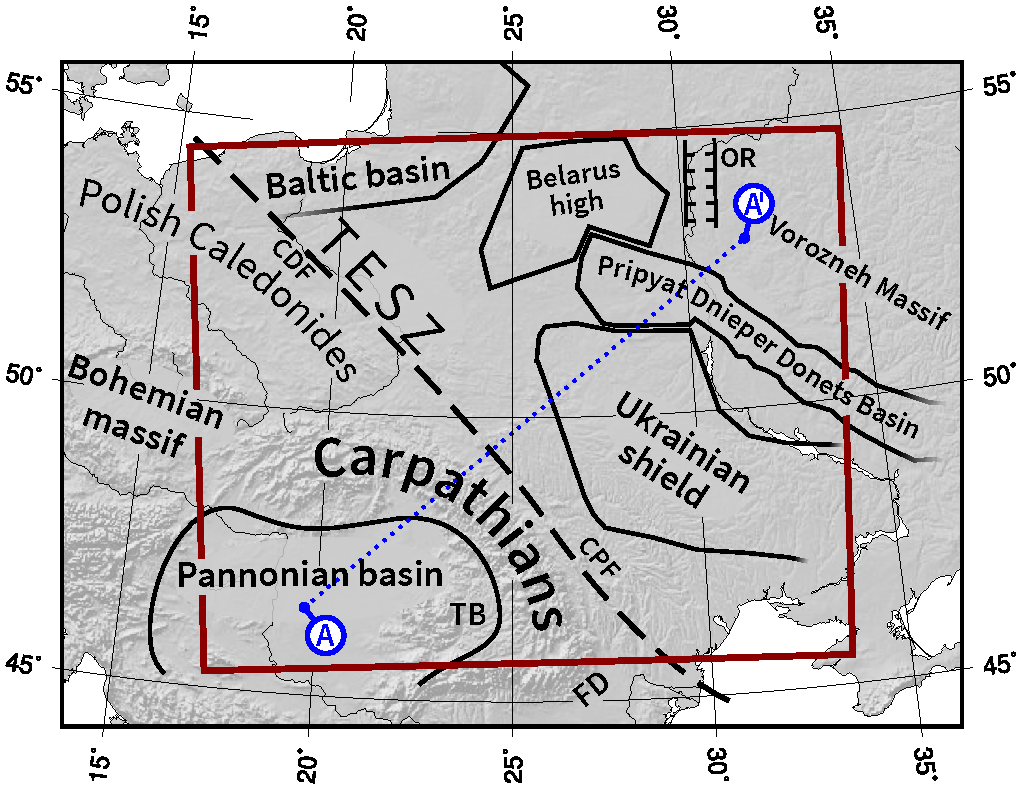
\includegraphics[width=1.2\textwidth]{./0400/geosetting.pdf}
    \end{adjustbox}
	\caption[Simplified map of the most significant geological units and boundaries inside the study area and in its proximity.]{Simplified map of the most significant geological units and boundaries inside the study area and in its proximity. The red rectangle encloses the extents of the Moho inversion result and of the thermal model. \textbf{TESZ}~Trans-European Suture Zone, \textbf{CDF}~Caledonides Foredeep, \textbf{CPF}~Carpathians Foredeep, \textbf{TB}~Transylvania Basin, \textbf{FD}~Focşani Depression, \textbf{OR}~Orsha Rift (Aulacogen). Data redrawn from \textcite{Tarapoanca2003}, \textcite{Tesauro2008}, \textcite{Artemieva2013}, \textcite{Mazur2016}, and \textcite{Starostenko2018}. Profile \textit{AA'} refers to the section shown in Fig.~\ref{fig:AAsection}.}
    \label{fig:geosetting}
\end{figure}

The method I am presenting consists of a gravity data reduction and Moho inversion phase, which I describe in section~\ref{s:Appl:Grav}, followed by a thermal modelling and parameter fitting phase, described in section~\ref{s:Appl:Therm}.
I have tested the procedure on a study area (Fig.~\ref{fig:geosetting} and~\ref{fig:extents}) in central-eastern Europe, encompassing different geological contexts and thermal regimes.
It is bounded by a box limited by \num{45}~to~\SI{55}{\degree N}, \num{15}~to~\SI{35}{\degree E}, transitioning from Phanerozoic lithosphere (Polish-German basin, Carpathians, Pannonian Basin) interested by extension events and orogeny to the Russian platform, crossing the Trans-European Suture Zone \parencite[TESZ,][]{Jones2010}.
In this area the available estimates of lithospheric thickness range from about 50~\si{\kilo \metre} to values in excess of 250~\si{\kilo \metre} across a steep transition zone, approximately 300~\si{\kilo \metre} wide.
This lithospheric geometry is overlaid by a remarkable assortment of crustal features.
These conditions result in a wide range of measured surface heat flow values (see section~\ref{ss:Appl:ThermInput}), ranging from 16 to 195~\si{\milli \watt \per \square \metre} (mean: 57~\si{\milli \watt \per \square \metre}).
The measurements towards the extremes of this range and short-wavelength variations were attenuated with a spatial-domain filter, since it is expected that they are arising from non-conductive heat transport (e.g. hydrology, shallow melts).
The regional grid of filtered surface heat flow measurements so obtained (see section~\ref{ss:Appl:DiscTherm:HF}) constitutes the dependent variable of the fitting procedure presented here.

\begin{figure}
    \begin{adjustbox}{center}
    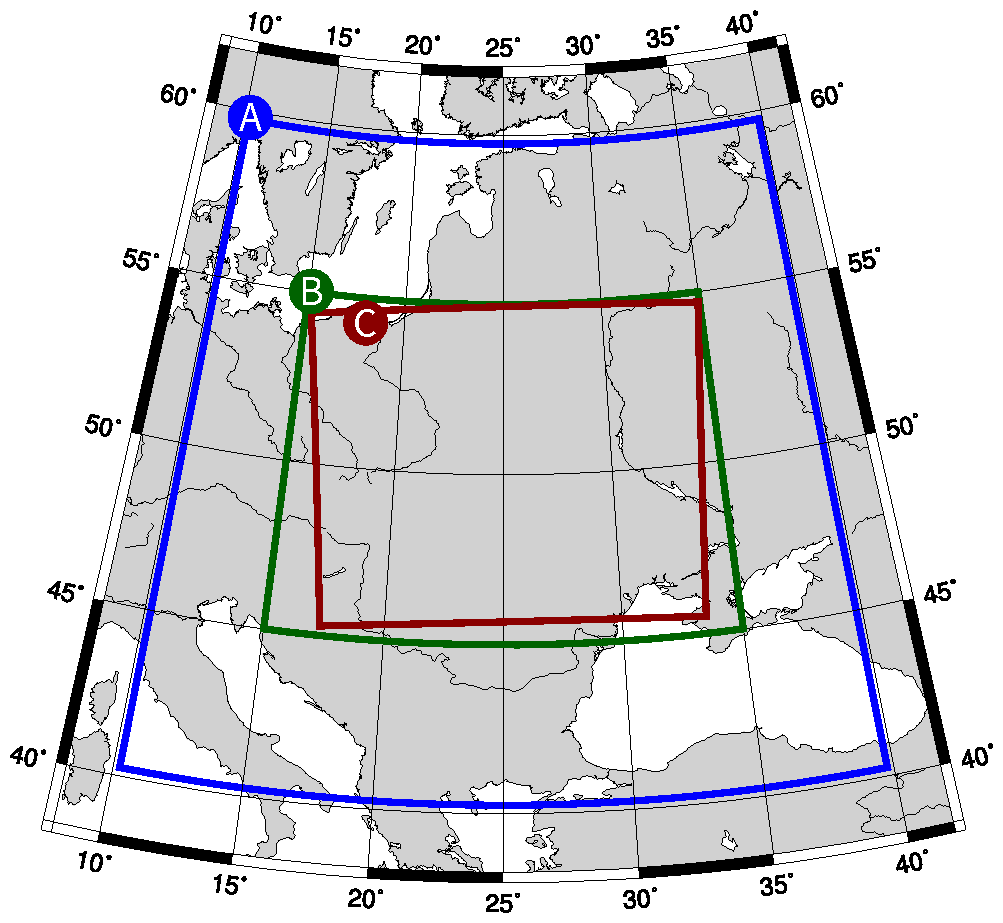
\includegraphics[width=1.2\textwidth]{./0400/extents.pdf}
    \end{adjustbox}
    \caption[Gravity modelling: extents of the modelled areas.]{Extents of the modelled areas. \textbf{A)} area outside of which the far-field gravity effect of crustal root (isostatic effect) was modelled. \textbf{B)} computation area for the gravity signal and reductions. \textbf{C)} extents of the inversion results and thermal model (UTM~35N grid).}
	\label{fig:extents}
\end{figure}

\section{Gravity model processing and inversion}
\label{s:Appl:Grav}

The crustal thickness estimation employed here is based on the solution of a gravity to Moho undulation inverse problem.
Its input signal is a reduced gravity disturbance from a global gravity model, which I pre-processed by computing and subtracting the contribution of topography, of far-field isostatic effects, and of the basement-to-topography sedimentary overburden.
With these reductions I aim at obtaining an anomalous gravity quantity, then interpreted as the effect of the varying depth of a crust-to-mantle boundary.

I have used the {GO\_CONS\_GCF\_2\_TIM\_r5} release \parencites{Brockmann2014}{Pail2011GOCE}{GOCETIMr5datasheet} of the global gravity model derived from the European Space Agency's \textit{Gravity field and steady-state Ocean Circulation Explorer mission} (GOCE), providing a ppm-level accuracy for $g$ with a half-wavelength resolution of about 70~\si{\kilo \metre} \parencite{Floberghagen2011_goce}.
This release comprises both GNSS tracking data --which dominate the gravity field solution up to spherical harmonic degree 30-- and observations of the on-board gradiometer, which cover the smaller spatial scales (higher degrees and orders).
The harmonic coefficients are obtained from these measurements through a least square regression for full normal equations complete to degree/order 150 for the GNSS and to 280 for the gradiometry.
A map of the gravity disturbance in the study area is shown in Fig.~\ref{fig:GGMmerged}~A.

\subsection{Reduction for the topographic and isostatic effects}
\label{ss:Appl:GravTopoIso}
I applied a global topography correction, computed as gravity disturbance, on a 15'~by~15' regular grid at 8~\si{\kilo \metre} above the GRS80 ellipsoid.
This was accomplished with the GrafLab software package \parencites{bucha2013GrafLab} and the spherical harmonics topography effect model {dV\_ELL\_RET2014} by \textcite{Rexer2016}, based on the {EARTH2014} global topography \parencite{Hirt2015}.
I then subtracted this from the GGM gravity disturbance computed on the same grid.
Both the spherical harmonics expansions where evaluated up to degree and order $280$.
The reduction density for the topography correction was 2670~\si{\kilo \gram \per \cubic \metre} for above-sea-level relief and 1030~\si{\kilo \gram \per \cubic \metre} for oceans.

% isostatic effect
As shown by \textcite{Szwillus2016}, the `global Bouguer anomaly' obtained with this procedure contains a significant long-wavelength bias due to the far-field effect of internal masses, including those involved in the isostatic compensation of topography (called \textit{isostatic effect}).
This is different from what would be obtained when processing local gravity data, using the `classic topographic reduction' computed inside a 167~\si{\kilo \metre} radius \parencite{hayford1912}.

I adopted one of the strategies suggested in \textcite{Szwillus2016}: accounting for the isostatic effect from masses outside of the study area.
I have chosen the {LITHO1.0} model \parencite{Pasyanos2014} as a global reference crustal root model.
By querying the `{access\_litho}' program point-wise on a global regular {0.125}~by~{0.125} degree grid, I extracted the crust-mantle boundary depth (`CRUST3' layer), its density, and $V_P$ in the lithospheric mantle (`LID' layer).

This procedure provided outlier values on some nodes.
I removed the values of crustal density and $V_P$ in the lithospheric mantle outside the range defined by three standard deviations around the mean (i.e. $\overline{x} \pm 1.5 \sigma $, with $\overline{x}$ mean value).
This implied keeping only the values of crustal density between 2500 and 3300~\si{\kilo \gram \per \cubic \metre} and of lithospheric mantle $V_P$ between 7500 and 8800~{m~s\textsuperscript{-1}}.
Crustal depths of less than zero or more than 80~\si{\kilo \metre} where also considered obvious interpolation artefacts, and removed.

I also compared each node value with a {1.5}~by~{1.5} degrees moving average (12 by 12 grid nodes). I have deleted the values with over 10~\si{\kilo \metre}, 200~\si{\kilo \gram \per \cubic \metre}, and 100~{m~s\textsuperscript{-1}} of absolute difference with the local moving average of depth, density, and $V_P$ respectively.
These criteria removed the {2.5}~\textperthousand~of the points sampled from {LITHO1.0}: 10198 points on a 1441~by~2881 global grid.
Linear interpolation was used to fill in the removed nodes.

This dataset was then low-pass filtered through convolution with a Gaussian kernel with a cut-off wavelength of 4~degrees, i.e. the wavelength at which the filter response value is $\exp(-0.5)$.
This equals to a {0.5} filter response at {3.4}~degrees.
This was applied as an anti-aliasing filter, prior to downsampling the depth and density data to a {0.5}~by~{0.5} grid.
With these three steps (oversampling, outlier processing, and low-pass filtering) of the data extracted from {LITHO1.0} I aimed at removing any artefacts that may arise due to re-gridding on a rectangular longitude-latitude grid.
Since the target is computing and removing a low degree effect, I consider such a drastic smoothing of input data justified.

I then blanked out the grid over a `study area' defined by 40 to 60 degrees latitude, 10 to 40 degrees longitude.
This area and subsequent crops, which I applied due to edge effects or re-projections, is shown in Fig.~\ref{fig:extents}.

This crustal root model was then discretised into {0.5}~by~{0.5} arc-degree wide spherical tesseroids \parencite{Uieda2016}, centred on the same sampling grid.
Each tesseroid density is equal to the contrast between the density of the lower crust and of the lithospheric mantle, against a reference Moho at {-35}~\si{\kilo \metre}.
For each grid node, this equals to:

\begin{equation}
	\label{eq:RhoContrast}
	\Delta \rho = \begin{cases}
		\rho_{C} - \rho_{M} & \mbox{if } D < \overline{D} \\ 
	    \rho_{M} - \rho_{C} & \mbox{if } D > \overline{D}
    \end{cases}
\end{equation}
with $D$ Moho depth, positive upwards, $\overline{D}$ reference depth, and $\rho_{C}$ crustal density as directly extracted from the model.
$\rho_{M}$, the mantle density, is provided constant at 3300{kg~m\textsuperscript{-3}} in {LITHO1.0} \parencite{Pasyanos2014}, although lateral variations in mantle velocity are provided.
I therefore follow the approach used by \textcite{Sebera2018}, applying the linear density-$V_P$ relation by \textcite{Yegorova2015}, which is based on {ACY400} \parencite{Montagner1989}:

\begin{equation}
	\label{eq:ACY400}
	\rho_M = 0.316 V_P + 769
\end{equation}
with $V_P$ in m/s and $\rho$ in {kg~m\textsuperscript{-3}}.

This yields an average contrast of 380~\si{\kilo \gram \per \cubic \metre}, which I note is lower than the global estimates of 485~\si{\kilo \gram \per \cubic \metre} by \textcite{Tenzer2012contrast} and of 448~$\pm$~187~\si{\kilo \gram \per \cubic \metre} by \textcite{Sjoberg2011}.
A globally uniform linear velocity-to-density conversion is a simplified model, which disregards the concurring effects of temperature, pressure and composition.
Nevertheless, I deemed it suitable to model a far-field, very long wavelength effect, which would be difficult to estimate otherwise \parencite[for a different approach, based on topography and the Airy-Heiskanen isostatic model, see][]{Grombein2016}.
Small scale variations are expected to be significantly smoothed out, while still obtaining a more refined and observation-based estimate than the one that would result from a high-pass filter on the gravity model (e.g. by setting the low degree and order coefficients to zero, up to an arbitrary cut off degree).

The gravity effect was computed through space-domain integration, using the Tesseroids program, version {1.2.1} \parencites{Uieda2016}{UiedaTesseroids}.
I computed the gravity field on a spherical grid, on a radius equal to the semi-major axis of the {GRS80} ellipsoid.
This field was then filtered and synthesised on the working grid according to the procedure described in section \ref{ss:Appl:GravSpectralFiltering}.
The result is shown in Fig.~\ref{fig:g_red}~B.

\begin{figure}
    \begin{adjustbox}{center}
	\fbox{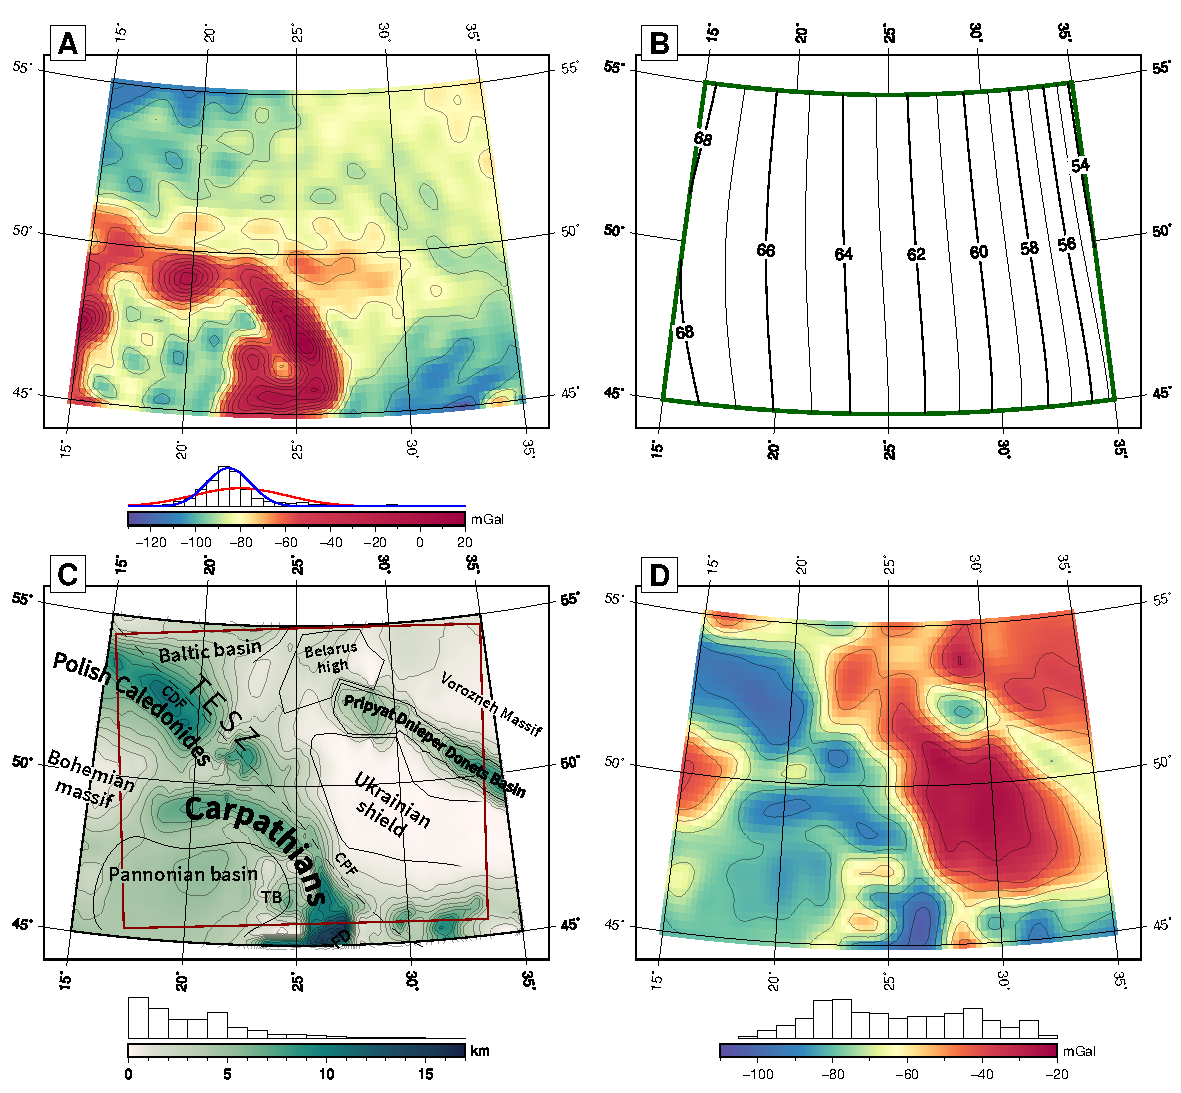
\includegraphics[width=1.2\textwidth]{./0400/reductions_merged.pdf}}
    \end{adjustbox}
	\caption[Data reductions to the gravity model.]{Data reductions to the gravity model.
	\textbf{A)}~Topographic effect (gravity disturbance) from the {RET2014} model \parencite{Rexer2016}. A median-centered normal fit is also plotted, in blue.
	\textbf{B)}~Forward-modelled far field gravity signal (radial component) due to isostatic compensation outside the study area.
	\textbf{C)}~Sediments thickness (km) in the study area, from \textcite{Tesauro2008}. Red rectangle: inversion results coverage. Geologic lineaments: see caption of Fig.~\ref{fig:geosetting}.
	\textbf{D)}~Sedimentary layer effect. Thicker sedimentary covers result in more negative values.
	Grid cells are shown on a 15' by 15' grid, without interpolation.}
	\label{fig:g_red}
\end{figure}

\subsection{Reduction for the sediment layer effect}
\label{ss:Appl:GravSed}
The low-density infill of sedimentary basins results in a negative bias of the Bouguer anomaly, since the topographic effect correction relies on the commonly used 2670~\si{\kilo \gram \per \cubic \metre} crustal reference density \parencite{Hinze2003}.
Since a negative density contrast is expected at the Moho, not accounting for this bias would result in an over-estimation of the crustal thickness.
I thus applied a \textit{sediment stripping correction} \parencite{Chen2014} to the gravity data, using the sediment thickness map provided in \textcite{Tesauro2008} in the study area (Fig.~\ref{fig:g_red}~C) and the rest of the European platform.
The rest of the Earth is covered by the sediment thickness data included in {LITHO1.0} by \textcite{Pasyanos2014}.
Using a global coverage enabled a realistic estimate of larger wavelengths.

The decrease in porosity (i.e. the volumetric ratio between grains and voids) due to compaction is modelled with the exponential model of \textcite{woodside1961}:

\begin{equation}
	\label{eq:ExpCompactionPhi}
	\phi(z) = \phi_0 \mathrm{e}^{-z/p}
\end{equation}
Where $z$ is depth (positive downwards), $\phi_0$ the porosity at the surface, and $p$ a characteristic skin-depth, such as $\phi(p) = \phi_0 \cdot \mathrm{e}^{-1}$.
Density can thus be computed with a porosity-weighted sum:

\begin{equation}
	\label{eq:ExpCompactionRho}
	\rho_{sed}(z) = [1-\phi(z)] \rho_{G} + \phi(z) \rho_{W}
\end{equation}
Where $\rho_{G}$ and $\rho_{W}$ represent the density of the grain matrix and of water filling the voids, respectively.

This reduction is critically dependent on two quantities: the estimates on the sedimentary cover thickness, and the spatial distribution of density in it.
Geological heterogeneities (e.g. lithology, basin history, cementation) result in deviations from general depth-compaction laws \parencite{allen2013basin}, hindering the reliability of universal trends.

I computed a sediment effect estimate using the following values: $\rho_G = \SI{2670}{\kilo \gram \per \cubic \metre}$, $\rho_W = \SI{1030}{\kilo \gram \per \cubic \metre}$ (brine), $\phi_0 = \num{0.5}$, $p = \SI{4}{\kilo \metre}$ ($1/p = \SI{0.25}{\per \kilo \metre}$).
This depth-density curve lies between the one provided for the Pannonian Basin by \textcite{Kaban2010} ($\phi_0 = \num{0.4}$, $p = \SI{2.375}{\kilo \metre}$), and the compaction behaviour of shaly sandstones provided in \parencite{allen2013basin} ($\phi_0 = \num{0.56}$, $p = \SI{2.5}{\kilo \metre}$).

This contribution was forward modelled with the same method used for the isostatic effect, through integration of discrete tesseroids.
I modelled the depth-wise density variation by dividing each tesseroid radially, with a step coarsening with depth (from 50~m at the surface to 200~m at 8~\si{\kilo \metre} of depth and more).
Each tesseroid density is equal to the contrast against a 2670~\si{\kilo \gram \per \cubic \metre} reference crustal density.
The result is shown in Fig.~\ref{fig:g_red}~D.

\subsection{Spectral-domain filtering of the computed reductions}
\label{ss:Appl:GravSpectralFiltering}
Subtracting the aforementioned reductions from a band-limited global gravity model carries the risk of introducing spectrally inconsistent higher degree components.
This is a consequence of adopting a space-domain forward modelling technique, which generates a band-unlimited gravity signal \parencite{Hirt2014}.
To remove any high-order component from the reductions, I carried out the following filtering procedure:
(1) first, every reduction signal was computed out globally, in terms of gravity field, on a spherical global grid of radius equal to {GRS80} semi-major axis.
This grid was an equally spaced grid ($N~\times~2N$) compliant to \textcite{Driscoll1994} sampling theorem.
(2) Then, I expanded it to a spherical harmonic expansion using {SHTOOLS} by \textcite{Wieczorek2018}. \nocite{SHTOOLS43Wieczorek2018}
(3) Using the same software, I synthesised the radial component of gravity from the spherical harmonics coefficients of the field. The SH series was truncated at maximum degree and order 280, and the values were calculated on an ellipsoidal surface, 8~\si{\kilo \metre} above GRS80.
This grid extends only over the study area.

\subsection{Inverse modelling}
\label{ss:Appl:GravInv}
I inverted for the crust-mantle interface (CMI) with the \textit{iterative constrained inverse modelling} routine included in the Lithoflex software \parencite{Braitenberg2007}, a method that has been extensively tested in similar schemes \parencites{Ebbing2001}{Mariani2013}.
Its algorithm alternates direct forward modelling and downward continuation, and has some analogies with the strategy of \textcite{Oldenburg1974}.

This procedure works in planar coordinates, therefore the obtained gravity signal was projected to a local coordinate reference system (WGS84 UTM zone 35N) on a 10~by~10~{km} grid.
The horizontal spatial resolution for the maximum degree ($N=280$) of the spherical harmonics expansion of the gravity model, defined as half of the minimum resolved wavelength, is about 71~\si{\kilo \metre}. This comes from the $\lambda_{min} \approx 40000~\textrm{km} / N $ rule \parencite{HofmannWellenhof2006}.
Therefore, the projected grid is oversampled with a factor of 7.1 with respect to the spatial resolution of the GGM.

The inversion parameters are $D$, the reference depth of the undulating interface, $P_{min}$, the minimum period of the raised cosine low-pass filter applied on the crustal root estimate, and $\Delta \rho$, the density contrast at the interface.
The first two parameters are uniform over all the input grid, while $\Delta \rho$ can vary horizontally.

$P_{min}$ is required for inversion stability and to attenuate any sharp Moho undulation that may result from inverting localised maxima and minima.
A value of 160~{km} was chosen to filter out short-wavelength Moho geometries which would be spectrally inconsistent with the resolving power of the gravity model.
$D$ and $\Delta \rho$ are not estimated by the inversion itself and require integration with external constraints.
I have extracted them from the global {LITHO1.0} model \parencite{Pasyanos2014}, adopting the average Moho depth in the study area (43.9~\si{\kilo \metre}) as $D$ and a 4-degree low-pass filtered Moho contrast, as computed in section \ref{ss:Appl:GravTopoIso}.
The density contrast map is shown in the right map of Fig.~\ref{fig:INVinput}.
Density is a temperature dependent parameter, due to the effect of thermal expansion \parencite{allen2013basin}.
Since the strategy presented here includes the temperature distribution in the lithosphere among the outputs, I could update the density model accordingly (using a thermal expansion model) and re-compute the Moho depth estimate, iteratively.
This has been tested for, resulting in local variations of up to \SI{3.4}{\kilo \metre}, with a standard variation of \SI{0.75}{\kilo \metre} after one iteration (see section~\ref{ss:ApplSup:MethodTests:MohoDeltaRho}).
Owing to the much larger uncertainties in Moho estimates \parencite[\textpm~5 to \textpm~15 percent, see ][]{Grad2009} and the additional parameter uncertainties involved, I opted to omit the thermal effect on density.

The use of a regional average Moho depth, different from the global reference depth of \SI{35}{\kilo \metre} (that I adopted to compute the global isostatic effect), is justified by the fact that I then subtracted the average gravity value over the area, before inversion.
Therefore, that average-free gravity anomaly is interpreted as deviations of the crust-mantle interface from the regional average depth.

\section{Thermal modelling}
\label{s:Appl:Therm}
The thermal modelling presented here is based on the assumption of steady state, three-dimensional heat conduction from the thermal-LAB to surface, on which the radioactive heat production is superimposed.

Both heat production and thermal conductivity are non uniform in the domain.
This means solving the heat equation for a inhomogeneous media, in the following vector form:
\begin{equation}
\label{eq:heateq}
\mathbf{\nabla} \cdot ( k(\mathbf{x}) \mathbf{\nabla} T(\mathbf{x}) ) = - A(\mathbf{x})
\end{equation}
With $k$ thermal conductivity (isotropic), $T$ temperature, $A$ heat production per unit of volume, and $\vec{x}$ position vector.
I solve eq.~\ref{eq:heateq} with a finite difference scheme on a rectilinear 3D domain, implemented in Matlab.
I adopt a planar approximation, which I deem suitable due to the small radial extent of the model (from the Earth surface to a depth of up to 205~\si{\kilo \metre}) in respect to its tangential extent (less than 10 by 20 arc-degrees, latitude by longitude).
Node spacing along the depth axis is non-uniform, to allow for a coarser resolution at higher depths.
A zero flux Neumann boundary condition \parencite{smith1985} is imposed along the vertical sides of the domain.

Upper and bottom boundaries are Dirichlet conditions \parencite{smith1985}, which I set to \SI{15}{\celsius} (surface temperature) and \SI{1200}{\celsius} (LAB temperature, see section~\ref{sss:Appl:ThermInputLAB}), respectively.
To accommodate for a non-flat morphology of these two boundaries, the Jacobian matrix coefficients of all nodes above topography or below the LAB are set to identities (i.e. the temperature of those nodes is fixed).
The solver input consists of the grid definition, the $\mathbf{k}$ and $\mathbf{A}$ arrays, and boundary conditions.
The finite difference system of linear equations is solved with Matlab built-in Cholesky decomposition for sparse arrays \parencite{Davis2006}.

\subsection{Thermal conductivity model}
\label{ss:Appl:ThermCond}
I adopt a reference thermal conductivity model of sediments, upper and lower crystalline crust and Sub-Continental Lithospheric Mantle (SCLM).
It includes standard values, at surface conditions, and models of their dependency on temperature and pressure.
Conductivity overall is strongly controlled by lithological properties such as mineralogy, porosity, free and bound water content \parencites{allen2013basin}{schon2011handbook}.
These properties in turn are highly variable parameters, due to the large crustal heterogeneity.
This a-priori reference may not describe the exact distribution of parameters in each of the model column.
It also should not be interpreted as a `mean model' of thermal conductivity in the study area, since it samples a local geological setting that is realistically expected to be significantly skewed in respect to a global average.
Nevertheless, it provides a reference, not unlike reference models used in seismic tomography -- deviations from it can be expressed as anomalies and it provides a consistent benchmark to perform comparison with other strategies.
The parameters and describing laws are summarised in Tab.~\ref{tab:ThermParams}.
They are described in the next sections.

\begin{table}
    \caption[Summary of the adopted thermal parameters.]{Summary of the adopted thermal parameters. For a detailed explanation of laws and symbols, refer to section~\ref{ss:Appl:ThermCond}. SCLM: Sub-Continental Lithospheric Mantle. Abbreviatiated sources: \textbf{V:}~\textcite{Vila2010}, \textbf{H:}~\textcite{Hasterok2011cont}, \textbf{C:}~\textcite{Chapman1986}, \textbf{X:}~\textcite{Xu2004}.}
    \begin{adjustbox}{center}
    \begingroup\setlength{\fboxsep}{0pt}
    \colorbox{tablebackground}{%
	\begin{tabular}{lll}
		\toprule
		 \textbf{Layer} & \textbf{Heat production ($\mathbf{A}$)} & \textbf{Thermal conductivity ($\mathbf{k}$)} \\
		\midrule
		\textbf{Sediments} & exponential compaction & exponential compaction [Eq.~\ref{eq:kSED}] \\
		& $\phi_0=\num{0.55}$, $p=\SI{2.5}{\kilo \metre}$, & $\phi_0$, $p$: same as $A$, \\
		& $A_{gr} = \SI{0.93}{\micro \watt \per \cubic \metre}$ [\textbf{V}], $A_{pf} = 0$ & $k_{gr} = \SI{3.0}{\watt \per \metre \per \kelvin}$, $k_{pf} = \SI{0.6}{\watt \per \metre \per \kelvin}$ \\
		\midrule
		\textbf{Upper crust} & initial guess $\SI{1.74}{\micro \watt \per \cubic \metre}$ [\textbf{V}] & temperature and depth dependent [\textbf{C}, Eq.~\ref{eq:kTzChap86}] \\
		& & $k_0=\SI{3.0}{\watt \per \metre \per \kelvin}$, \\
		& & $b=\SI{1.5e-3}{\per \celsius}$, $c=\SI{1.5e-6}{\per \metre}$ \\
		\midrule
		\textbf{Lower crust} & initial guess $\SI{0.37}{\micro \watt \per \cubic \metre}$ [\textbf{V}] & temperature and depth dependent [\textbf{C}, Eq.~\ref{eq:kTzChap86}]\\
		& & $k_0=\SI{2.6}{\watt \per \metre \per \kelvin}$, \\
		& & $b=(\SI{1.0e-4}{\per \celsius}$, $c=\SI{1.5e-6}{\per \metre}$ \\
		\midrule
		\textbf{SCLM} & $\SI{0.02}{\micro \watt \per \cubic \metre}$ [\textbf{H}] & temperature and pressure dependent, sum of: \\
		& & - lattice conduction term [\textbf{X}, Eq.~\ref{kLat}] \\
		& & - radiative term [\textbf{H}, Eq.~\ref{kRad}] \\
		\bottomrule
    \end{tabular}
    }\endgroup
    \end{adjustbox}
	\label{tab:ThermParams}
\end{table}

% SEDIMENTS
\subsubsection{Sediments}
\label{sss:Appl:ThermCondSed}
The thermal conductivity in the sedimentary layer follows the same exponential compaction model adopted for the sediment reduction to the gravity signal (equation \ref{eq:ExpCompactionPhi}). Therefore, the bulk sediment conductivity can be modelled as a porosity-weighted sum of the conductivities of the rock matrix (grains, $k_{gr}$) and the pore-filling fluid ($k_{pf}$) \parencites{woodside1961}{allen2013basin}:

\begin{equation}
\label{eq:kSED}
k_{sed}(z) = [1-\phi(z)] k_{gr}+ \phi(z) k_{pf}
\end{equation}
The porosity-depth compaction curve is the same used for the gravity modelling.
I adopt a thermal conductivity of the solid matrix ($k_{gr}$) and of the pore fluid ($k_{pf}$, assumed brine) equal to \SI{3.0}{\watt \per \metre \per \kelvin} and \SI{0.6}{\watt \per \metre \per \kelvin}, respectively \parencite{Revil2000}.

% CRUST
\subsubsection{Crystalline crust}
\label{sss:Appl:ThermCondCrust}
I model the inverse dependence between temperature and thermal conductivity in the crystalline continental crust with the empirical relationships proposed by \textcite{Chapman1986}:

\begin{equation}
\label{eq:kTzChap86}
k(T,z) = k_0 (1+cz) / (1+bT)
\end{equation}
where $k_0$ is the measured conductivity at surface standard conditions (\SI{273.15}{\kelvin} and \SI{e5}{\pascal}), and $c$ and $b$ are two parameters expressing the dependency on depth and pressure, respectively.

\subsubsection{Sub-continental lithospheric mantle}
\label{sss:Appl:ThermCondSCLM}
Owing to the higher temperatures reached in the SCLM, the effect of heat transfer by means of black body radiation cannot be overseen.
Along with the scarceness of direct samples (i.e. mantle xenoliths), this makes the estimation of thermal conductivity in the SCLM a difficult task, requiring a refined modelling of the behaviour of the lattice of each mineral phase under mantle conditions \parencite{Hofmeister1999}.
While there is consensus on the reliability of the relationship between the tectonothermal age of the crust and the composition of the underlying lithospheric mantle \parencites{Afonso2008}{Griffin2009}, estimating the mineral assemblage given the pressure and temperature conditions requires an adequate thermodynamic modelling \parencite[e.g][]{Guerri2015}, which is outside the scope of this work.

I thus assume a reference SCLM, defined by its thermal conductivity at surface conditions and a model of its temperature and pressure dependency.
Thermal conductivity at depth is influenced by the superposition of a lattice effect --directly proportional to pressure and inversely proportional to temperature-- and a radiative contribution --directly proportional to temperature, i.e. $k = k_{lat}(P,T) + k_{rad}(T)$.
I adopt the lattice thermal conductivity ($k_{lat}$) model by \textcite{Xu2004}, using the values provided for Olivine in the 4 to 10~GPa range:

\begin{equation}
	\label{kLat}
	k_{lat} = k_{298} \left( \frac{298}{T} \right)^n (1+ a P)
\end{equation}
where $T$ is temperature in \si{\kelvin}, $k_{298}$ the lattice conductivity at \SI{298}{\kelvin} (\SI{4.13}{\watt \per \metre \per \kelvin}), $n$ an empirical fitting factor ($0.5$), $a$ the pressure dependency factor (\SI{0.032}{\per \giga \pascal}), and $P$ pressure in \si{\giga \pascal}.
I computed $P$ as a purely lithostatic pressure, by utilising the same sediment model used in the gravity reduction, a reference crust density of 2670~\si{\kilo \gram \per \cubic \metre}, and the same lithospheric mantle density that I calculated in Eq.~\ref{eq:ACY400}.

I account for the radiative component ($k_{rad}$) by adopting the model of \textcite{Hasterok2011cont}:

\begin{equation}
	\label{kRad}
	k_{rad} = \frac{1}{2} k_{rad}^{max}  \left[ 1 + \mathrm{erf} \left( \frac{T-T_R}{\omega} \right) \right]
\end{equation}
Here the parameters are: $k_{rad}^{max}$ maximum radiative conductivity (\SI{0.345}{\watt \per \metre \per \kelvin}), $T_R$ reference temperature (i.e. the temperature at which $0.5 \cdot k_{rad}^{max}$ is reached, \SI{762}{\kelvin}), and a scaling factor $\omega$ (\SI{256}{\kelvin}).
The error function is denoted with $\mathrm{erf}$.

\subsubsection{Temperature dependency of thermal conductivity}
\label{sss:Appl:ThermCondTdep}
The temperature dependency of $k$ introduces a non-linearity and is thus accounted for iteratively, using subsequent substitution \parencite[or ``Picard's method'', e.g. ][]{Hauck1999}.
The starting condition is a linear geotherm from surface temperature to \SI{1200}{\celsius} LAB \parencite{fischer2010lab}.
After three iterations (i.e. when calculating the thermal conductivity using the temperature output of the second iteration) the procedure converges to less than \SI{1}{\kelvin} variations in temperature and less than {0.4}~\si{\milli \watt \per \square \metre} variations in surface heat flow.
See section~1 of the Supplementary Material for a test on the behaviour of this method.

\subsection{Iterative fit of heat generation}
\label{ss:Appl:ThermRHP}
Lacking direct measurements of radioactive heat production (RHP) throughout the whole crust thickness, estimates commonly rely on compilations of compositional data, e.g. \textcites{Vila2010}{Artemieva2017granite}{Hasterok2017_ign}{Hasterok2017_mis}.

The depth-wise distribution of radioactive elements is poorly modelled by simple functions \parencite{Jaupart2003} and is difficult to constrain from indirect observables.
A decay with depth at large scale is commonly expected, owing to the progressive depletion of the lowermost crustal terms.
Still, this model is challenged by evidence of heat-producing element rich bodies in the lower crust \parencite{Alessio2018deepRHP}, which suggest reconsidering the role attributed to crustal-scale differentiation.
I therefore resort to using one bulk heat production for the whole crystalline crust, using an initial value that I derive from the lithotype medians reported in \textcite{Vila2010} and the reference crustal column of \textcite{Wedepohl1995}.

This initial value of bulk heat production is then fitted to the measured surface heat flow, in cells where it is available, using the following scheme.
The misfit between the forward-modelled surface heat flow and the measured one ($\Delta Q_0$) is divided by the crustal thickness ($z_{Moho} - z_{Sed}$), thus converting the heat flow misfit in a heat production per unit of volume value.
I use this to guess a new bulk crustal heat production ($A$).
For the $n$th iteration, in the crustal column identified by $u, v$ grid position, this can be expressed as:

\begin{equation}
	\label{eq:IterativeRHP}
	A_n^{u,v} = A_{n-1}^{u,v} + \Delta Q_0^{u,v} / (z_{Moho} - z_{Sed})^{u,v}
\end{equation}
The resulting $A_n^{u,v}$ is then partitioned according to the upper to lower crust thickness ratio of \textcite{Wedepohl1995} column (thickness ratio upper to lower crust = 0.485).
This method constitutes an iterative subsequent substitution scheme.
It is similar to the strategy adopted by \textcite{Cermak1986}, where the unknown was the the heat flow at the base of the model.
That method was subsequently referred to as a `pseudo-inverse' technique \parencite{Cermak1993}.

The RHP in cells where no surface heat flow measurements are available is filled in by interpolating the fitted RHP values, using a natural neighbour interpolation \parencite{Sibson1981}.
Undulations in crustal thickness are not accounted for when performing this interpolation.

Note that in a model with only one-dimensional heat conduction (along the vertical axis) and no temperature-conductivity dependence, this would lead to an exact solution in only one iteration.
Horizontal heat conduction results in thermal gradient deviations around an hotter (more radioactive) crust, and the decrease in thermal conductivity for a larger temperature enhances this effect (for a synthetic example, see section~2 of the Supplementary Material).

The radioactive heat production in the solid matrix of sediments is fixed at \SI{0.93}{\micro \watt \per \cubic \metre}, from \textcite{Vila2010}, and follows the same exponential compaction law of thermal conductivity.
I set $A$ in the lithospheric mantle to \SI{0.02}{\micro \watt \per \cubic \metre} \parencite{Hasterok2011cont}.

\subsection{Thermal model input data}
\label{ss:Appl:ThermInput}

\subsubsection{Surface heat flow}
\label{sss:Appl:ThermInputSHF}

I based this work on the data available in the Global Heat Flow Database of the International Heat Flow Commission, as available in the version maintained by \textcite{globalHF}.
The raw records included 2780 points inside the study area (Fig.~\ref{fig:HFdata}, A).
I edited them by discarding samples with heat flow above 300~\si{\milli \watt \per \square \metre} (5~points in the \SI{2.5}{\degree}~buffer around the study area, no points inside the study area) and below 15~\si{\milli \watt \per \square \metre} (23~points in the buffer, 3~points inside the study area).
Due to the whole-crust scale of this work compared with the typical measurement depth (less than a kilometre), no depth correction was applied to the records.
I also did not apply any correction for the paleoclimatic effect, which in the area has been estimated ranging from \num{0}~to\SI{20}{\milli \watt \per \square \metre} by \textcite{Majorowicz2011}.

I corrected the records for the sampling bias toward high heat flow spots \parencite{Mareschal2013} and the short-wavelength components that may arise from near-surface phenomena.
First, the study area is divided in a graticule of \num{40}$\times$\SI{40}{\kilo \metre} grid step, in local projected coordinates (UTM35N), and the median surface heat flow for each cell is calculated.
Then the heat flow grid, which is treated as node-registered array, is convolved with a raised cosine kernel (the same kind used in the Moho inversion algorithm), resulting in a low-pass filtered heat flow grid.
The filter kernel was sized for a cut-off wavelength of \SI{320}{\kilo \metre}, twice the cut-off applied to the Moho undulations.

The processed surface heat flow grid (shown in Fig.~\ref{fig:HFdata}, B) constitutes the input of the iterative accommodation of bulk crustal heat production, as described in section \ref{ss:Appl:ThermRHP}.

\subsubsection{Lithosphere-Asthenosphere Boundary}
\label{sss:Appl:ThermInputLAB}

I extracted the bottom boundary condition, a \SI{1200}{\celsius} LAB-isotherm, from the lithospheric thickness estimates provided in LITHO1.0 by \textcite{Pasyanos2014}, which are obtained from the inversion surface wave dispersion data.
The points were interpolated to a regular grid with a bilinear 2D spline interpolator \parencite{Wessel2009}, finding an approximate fit explaining 99.9\% of the input data variance.
The data and the interpolated extents are shown in Fig.~\ref{fig:LAB}.

\begin{figure}
	\begin{adjustbox}{center}
	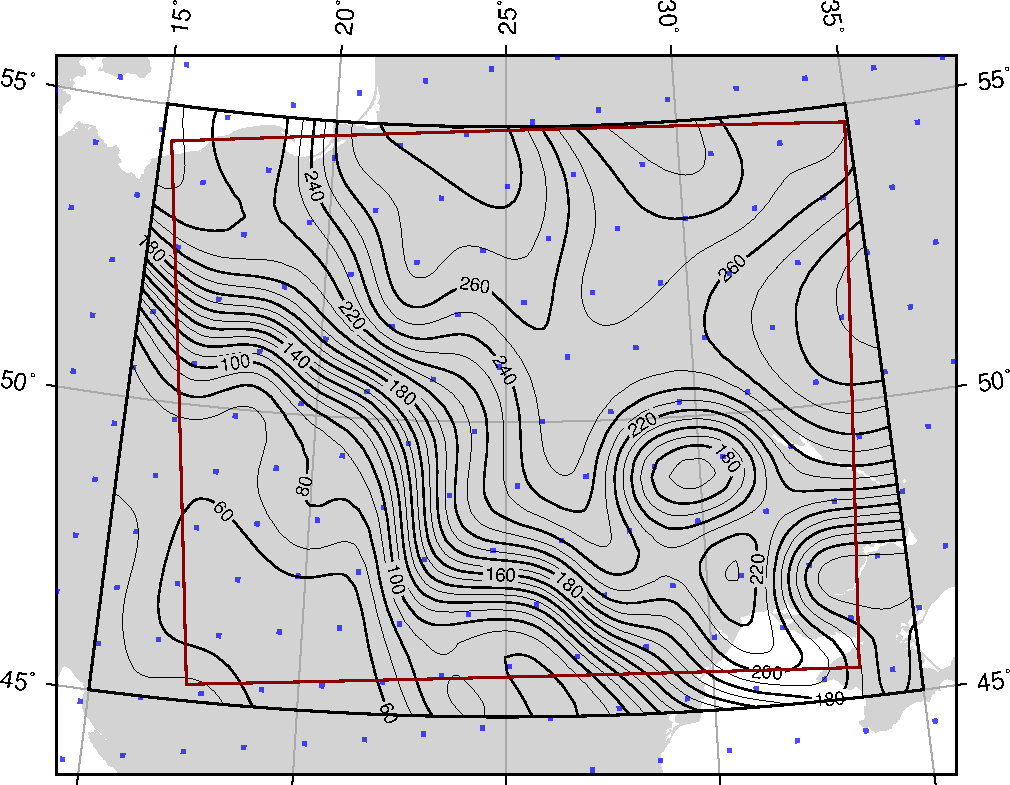
\includegraphics[width=1.2\textwidth]{./0400/LAB_LITHO.pdf}
	\end{adjustbox}
	\caption[Depth of lithosphere-asthenosphere boundary (LAB), as provided in LITHO1.0.]{Depth of lithosphere-asthenosphere boundary (LAB) in km, as provided in LITHO1.0 \parencite{Pasyanos2014}. \textbf{Black polygon:}~interpolation extents. \textbf{Red polygon:}~extents of the thermal model. \textbf{Blue squares:}~LITHO1.0 data nodes.}
	\label{fig:LAB}
\end{figure}

The chosen temperature is an approximation arising from the thermal definition of the lithosphere: a thermal boundary layer, where heat transport is purely conductive, overlying a convecting mantle \parencites{Eaton2009}{fischer2010lab}.
This boundary temperature is therefore tied to a rheological definition, separating the mantle from the rigid lithospheric domain, where convection is not sustainable and tectonic plates move coherently \parencite{Steinberger2016}.
Common choices range from the mantle solidus temperature, which is pressure- and composition-dependent, to fractions of it, due to the evidence that even comparatively small melt percentages result in the seismic velocity drop associated with the LAB.
The heat flow sensitivity to the chosen LAB temperature is small in respect to uncertainties in heat flow measurement or modelling -- therefore, a thermal-LAB depth inverted from surface heat flow has an associated error in the order of tens of kilometres \parencite{Afonso2013multiobsI}.
When tested in the forward modelling setup, the difference in terms of Moho heat flow of a thermal-LAB temperature of \SI{1300}{\celsius} versus \SI{1200}{\celsius} is 1.44~\si{\milli \watt \per \square \metre}, for the same 150~\si{\kilo \metre} deep LAB ($Q_M$ of 17.05 and 15.61~\si{\milli \watt \per \square \metre}, respectively).

\textcite{Pasyanos2014} included prior information in their surface wave inversion, as a starting model which was then perturbated.
This data includes ``tectonic regions, crustal thickness from receiver functions and other information, upper mantle velocities from traveltime models, and thermotectonic information'' \parencite[p. 2154, ][]{Pasyanos2014}.
I have preferred this model over other single-observable LAB models available in the area --e.g. receiver functions \parencite{Geissler2010}, tomography inversion \parencite{Tesauro2009}, seismic anisotropy \parencite{Plomerova2010}.
A degree of dependence on prior data, including thermal models and Moho depth estimates, is unavoidable, since a common aspect of different techniques is requiring a correction for crustal effects \parencite{Jones2010}.
The adopted model provides a uniform coverage at an acceptable scale for the thermal footprint of LAB undulations, with a satisfactory resolving power of local features, such as the thin lithosphere underneath the Pannonian Basin (\SI{50}{\kilo \metre}).

\section{Results of gravity reduction and inversion}
\label{s:Appl:DiscGrav}

\subsection{Gravity reductions}
\label{ss:Appl:DiscGravReductions}

Using the procedure described in section~\ref{s:Appl:Grav}, I started from the gridded GOCE-GGM input signal shown in Fig.~\ref{fig:GGMmerged}~A) and obtained a reduced signal, shown in Fig.~\ref{fig:GGMmerged}~B), through subtraction of the effects of global topography (Fig.~\ref{fig:g_red}~A), far isostatic roots (Fig.~\ref{fig:g_red}~B), and sediments (Fig.~\ref{fig:g_red}~D).
A histogram is plotted under each gravity signal map, its width coinciding with the colour-scale width.
A continuous normal distribution, computed using the mean and standard deviation of the plotted data, is overlaid on each histogram.
These two plots serve as a qualitative indicator of the signal distribution, while the quantitative statistics are shown in Tab.~\ref{tab:GravDescrStats}.

\begin{figure}
    \begin{adjustbox}{center}
	\fbox{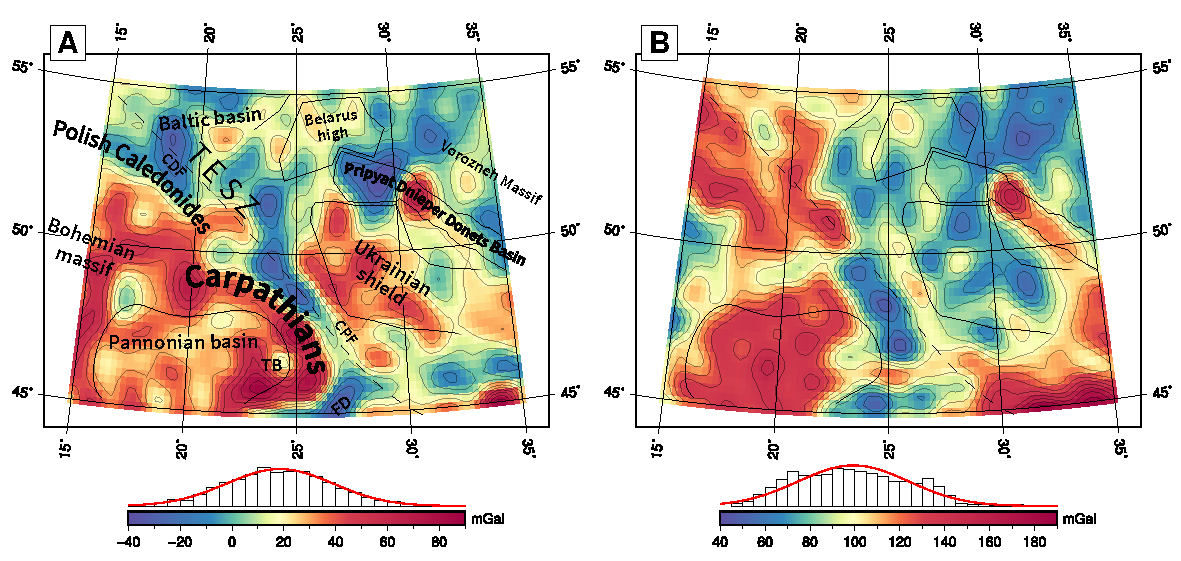
\includegraphics[width=1.3\textwidth]{./0400/GGM_merged.pdf}}
    \end{adjustbox}
	\caption[Input and processed gravity data.]{Input and processed gravity data.
	\textbf{A)}~Gravity disturbance, computed from the global gravity model {GO\_CONS\_GCF\_2\_TIM\_r5}, at \SI{8}{\kilo \metre} over GRS80.
	\textbf{B)}~Sediment-reduced Bouguer anomaly, obtained by subtracting the topography, isostatic and sediment reductions from the GGM gravity disturbance.
	Grid cells are shown on a 15' by 15' grid, without interpolation. \SI{1}{mGal} = \SI{e-5}{\metre \per \square \second}.}
	\label{fig:GGMmerged}
\end{figure}

\begin{table}
    \caption[Descriptive statistics of the input gravity signal, of its reductions, and of the inversion results.]{Descriptive statistics of the input gravity signal, of its reductions, and of the inversion results (Moho depth and gravity residuals). GD: gravity disturbance, from the global gravity model. LPF: raised cosine low-pass filter, applied during the inversion algorithm.}
    \begin{adjustbox}{center}
    \begingroup\setlength{\fboxsep}{0pt}
    \colorbox{tablebackground}{%
	\begin{tabular}{lcrrrrr}
		\toprule
		 & & \textbf{Min} & \textbf{Max} & \textbf{Mean} & \textbf{Median} & \textbf{St. Dev.} \\
		 \midrule
		\textit{Input data} \\
		\quad GD, unprocessed & mGal & -38.0 & 87.6 & 18.5 & 18.1 & 20.6 \\
		\quad Topographic effect & mGal & -121.5 & 19.6 & -80.4 & -85.4 & 20.7 \\
		\quad Isostatic effect & mGal & 53.6 & 69.0 & 62.4 & 62.8 & --- \\
		\quad Sediments thickness & km & 0 & 16.3 & 3.1 & 2.6 & 2.6 \\
		\quad Sediments effect & mGal & -104.5 & -24.1 & -62.8 & -65.0 & 19.7 \\
		\quad GD, reduced & mGal & 46.77 & 186.6 & 99.3 & 98.8 & 24.6 \\
		\quad GD, reduced, mean removed & mGal & -52.5 & 87.3 & 0 & -1.2 & 24.6 \\
		\textit{Inversion results} \\
		\quad Inverted Moho depth (no LPF) & km & 23.2 & 81.5 & 44.2 & 43.7 & 4.9 \\
		\quad Inverted Moho depth (160 km LPF) & km & 34.2 & 51.7 & 44.2 & 44.0 & 2.6 \\
		\quad Residuals (no LPF) & mGal & -1.8 & 1.7 & 0.0 & 0.0 & 0.2 \\
		\quad Residuals (160 km LPF) & mGal & -19.6 & 17.2 & 0.1 & 0.2 & 5.2 \\
		\bottomrule
    \end{tabular}
    }\endgroup
    \end{adjustbox}
	\label{tab:GravDescrStats}
\end{table}

The cumulative effect of the reductions shifted the gravity signal towards positive values, resulting in a 80.8~mGal increase of the average value.
The global topography effect (Fig.~\ref{fig:g_red}~A) is negative over most of the study area, except the most central parts of large high topography areas: the Carpathians (centre-south of the study area), the Bohemian massif, and the easternmost portion of the Alps, at the western edge of the study area.
The average topography in the area, from the {EARTH2014} model at full resolution, is 220~m.
It ranges from -113~m (small northern portion of the Black Sea, sampled on the southern edge) to 2109~m (Mt.~Moldoveanu, SE Carpathians).

The crustal root effect outside of the study area (`isostatic effect', Fig.~\ref{fig:g_red}~B) is dominated by a east-west negative gradient, ranging from 68 to 54~mGal over a 20~degrees longitude range.
The north-south gradient is negligible.

The sediment thickness (Fig.~\ref{fig:g_red}~C) ranges from zero to 16.3~\si{\kilo \metre}, with an average of 3.1~\si{\kilo \metre}.
The western half of the area is characterised by thick sedimentary covers: between the Caledonides Foredeep and the Baltic Basin (NW corner, 11~\si{\kilo \metre} maximum), and along the Carpathians Foredeep, up to the very deep, but localised, Focşani Depression (16.3~\si{\kilo \metre} maximum).
The Pripyat-Dnieper-Donets basin lies in the north-eastern part of the area.
Basement depth reaches a maximum of 5~\si{\kilo \metre} there.
The forward-modelled sediments effect, reaches a maximum of -102~mGal using the aforementioned compaction parameters.
The depth-dependent exponential decay of compaction implies that the highest sensitivity of the gravity effect occurs in the first 6--8~\si{\kilo \metre} of thickness, where both the basement depth and the density modelling are critical, with the variance in the latter dominating the gravity signal \parencite{Kaban2010}.

The gravity footprint of masses at distance is such that the minimum sediment effect value is \SI{-24.7}{mGal}, instead of zero, even over areas with little to no sedimentary cover.

I assumed a uniform sediment compaction model and a set of depth-dependence parameters which, albeit a realistic compromise, does not reflect the exact characteristics of any of the basins in the study area.
This unmodelled variability is a source of uncertainty, which is usually addressed with integration with local well data, where available.
The depth-density curve that \textcite{Kaban2010} provide for the Pannonian Basin is defined by $\phi_0 = 0.4$ and $p = 2.375$~{km}, while the parameter used here are $\phi_0 = 0.5$ and $p = 4$~{km}.
Their \parencite{Kaban2010} curve describes sediments which are less porous at the surface and that compacted faster with increasing depth.
This means that for the same sediment thickness, a smaller gravity correction is obtained.

The sediment correction computed over the entire study area with those parameters is on average \SI{22.8}{mGal} smaller, up to a maximum of \SI{48.8}{mGal}, over the absolute maximum of sediment thickness, the aforementioned Focşani Depression.
The standard deviation of the difference is \SI{9.4}{mGal}.
Over the Pannonian Basin (about \SI{5.2}{\kilo \metre} of sediments), the correction using \textcite{Kaban2010} parameters is \SI{33}{mGal} smaller.
Therefore, the inverted crustal thickness using \textcite{Kaban2010} compaction model is consistently thicker, on average by \SI{842}{\metre}.
Resorting again to the Pannonian Basin as a benchmark, the estimate with those parameters is up to \SI{2.4}{\kilo \metre} thicker.
In absolute terms, this means that the adopted compaction model results in a \SI{39.0}{\kilo \metre} Moho there, while their \textit{basin-specific} one results in \SI{41.2}{\kilo \metre} --even the less compacted model that I adopted is not enough to fully explain the Pannonian Basin thinning sensed by other crustal models, as it is discussed afterwards (section~\ref{ss:Appl:DiscGravComp}).

\subsection{Moho estimate}
\label{ss:Appl:DiscGravMoho}

\begin{figure}
	\begin{adjustbox}{center}
	\fbox{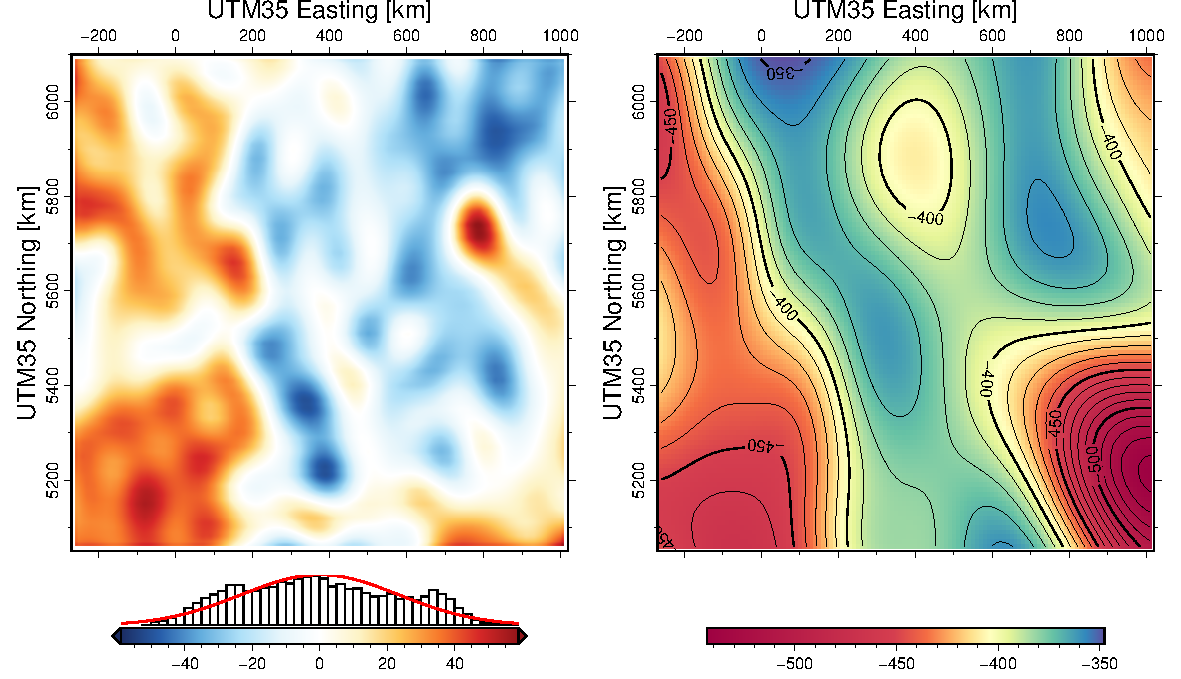
\includegraphics[width=1.2\textwidth]{./0400/UTMinv.pdf}}
	\end{adjustbox}
	\caption[Inversion input, projected to a 10~by~\SI{10}{\kilo \metre} UTM35N grid.]{Inversion input, projected to a 10~by~\SI{10}{\kilo \metre} UTM35N grid. \textbf{Left:}~Inversion input gravity signal, in mGal. \textbf{Right:}~Moho density contrast (kg~m\textsuperscript{-3}) used in inversion, derived from {LITHO1.0} \parencite{Pasyanos2014} and the linear $V_P$ to SCLM density relationship by \textcite{Yegorova2015}.}
	\label{fig:INVinput}
\end{figure}

The left map of Fig.~\ref{fig:INVinput} shows the input data for the inversion routine.
The dataset was obtained by removing the mean value of the reduced gravity signal and projecting it on a local UTM grid.
Removing the mean value complies with the fact that the reference depth is equal to the expected Moho average depth.
This way I interpret the reduced input gravity signal as due to deviations of the crust-mantle interface from its average value in the study area.
The inversion result, re-projected to WGS84 coordinates, is shown in Fig.~\ref{fig:INVMoho}.
Loss of edges occurs due to convergence of meridians, since the projection to the UTM grid is cropped to a rectangular domain (the extents are compared in Fig.~\ref{fig:extents}, area B and C).
The 160~\si{\kilo \metre} low-pass filter results in residuals (i.e. the difference between the input gravity signal and the forward-modelled signal of the Moho estimate) ranging from -19.6 to 17.2~mGal, shown in Fig.~\ref{fig:INVResMoho}.
As shown in the statistics of Tab.~\ref{tab:GravDescrStats}, the residuals are negligible when no Moho low-pass filter is applied.
This comes at a cost for the Moho estimate morphology, which exhibits local spikes of up to 23.2~\si{\kilo \metre} (minimum depth) and 81.5~\si{\kilo \metre} (maximum depth) before filtering.
The final RMS misfit at the 10\textsuperscript{th} iteration of the inversion algorithm is of 4.96 and 0.24~mGal with and without low-pass filtering, respectively.

\begin{figure}
	\begin{adjustbox}{center}
	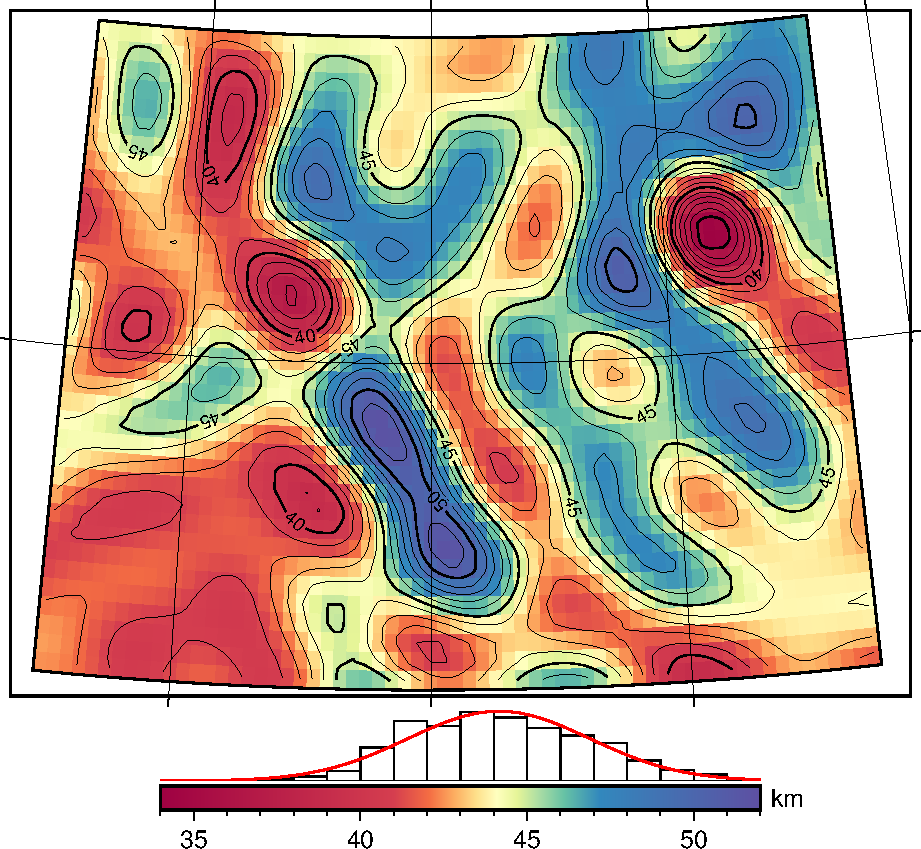
\includegraphics[width=\textwidth]{./0400/MohoWGS.pdf}
	\end{adjustbox}
	\caption[Moho depth as obtained from the inversion.]{Moho depth as obtained from the inversion, contour interval 1~\si{\kilo \metre}. Some of the geological features of Fig.~\ref{fig:geosetting} are shown: \textbf{TESZ}~Trans-European Suture Zone, \textbf{CDF}~Caledonides Foredeep, \textbf{CPF}~Carpathians Foredeep, \textbf{TB}~Transylvania Basin, \textbf{PB}~Pannonian Basin, \textbf{PDDB} Pripyat-Dnieper-Donets basin, \textbf{BB}~Baltic Basin.}
	\label{fig:INVMoho}
\end{figure}

\begin{figure}
	\begin{adjustbox}{center}
	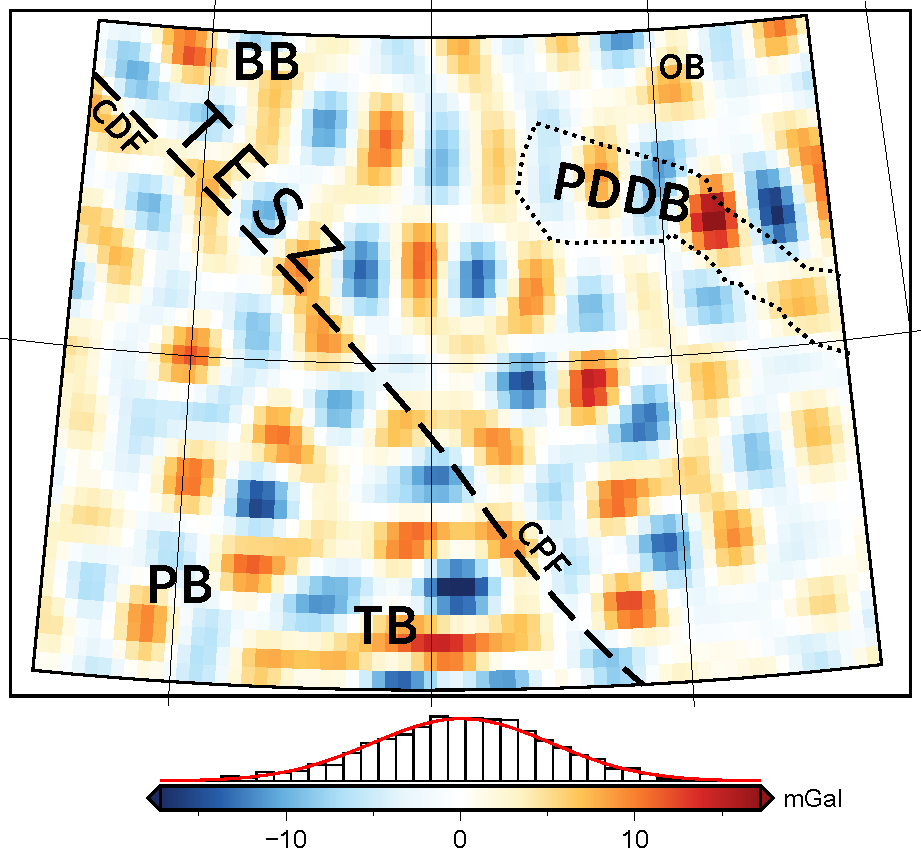
\includegraphics[width=\textwidth]{./0400/MohoResWGS.pdf}
	\end{adjustbox}
	\caption[Inversion residuals: input gravity signal minus forward-modelled Moho undulation effect.]{Inversion residuals: input gravity signal minus forward-modelled Moho undulation effect. Labelled features: see Fig.~\ref{fig:INVMoho}.}
	\label{fig:INVResMoho}
\end{figure}

The Moho estimate that I obtained from inversion exhibits a thickening under the East Carpathians up to 51.7~\si{\kilo \metre} and up to \SI{46.4}{\kilo \metre} under their north-west portion.
The two sectors are interrupted by a relatively shallow saddle (\SI{44.2}{\kilo \metre}) at \SI{49}{\degree N} \SI{22}{\degree E}.

A dominant north-west to south-east lineament is observed in the whole area, parallel to the TESZ.
This could be discerned already in the input data, even before integration with the {LITHO1.0} density contrast, which too shows a sharp NW-SE gradient across the suture zone.

Crustal thinning  in the Caledonides Foredeep (CDF) and the Baltic Basin (BB), in the north-west sector of the area, reaches \SI{38.0}{\kilo \metre}.
Underneath the longitudinally central part of the Pripyat-Dnieper-Donets Basin (PDDB), the Moho rises up to 34.2~\si{\kilo \metre} locally. This thinning coincides with the Chernigov High, attributed to lower crustal mafic intrusions \parencite{Starostenko2018}.
Relatively thin crust (not exceeding \SI{41.1}{\kilo \metre}) persists eastwards of this local minimum, following the basin shape.
It is interrupted westwards, instead, by a \SI{48}{\kilo \metre} thick lineament orthogonal to the basin longitudinal axis.

I observe a thin crust under the Pannonian Basin (PB, south-west corner of the study area), never exceeding \SI{41.8}{\kilo \metre} and reaching a local minimum of \SI{38.9}{\kilo \metre} at \SI{48}{\degree N} \SI{22.75}{\degree E}.

\subsection{Comparisons and critical aspects}
\label{ss:Appl:DiscGravComp}

I adopt three different crustal models as benchmarks for the inverted Moho depth estimate: the European Moho depth by \textcite{Grad2009}, the global GOCE-based model GEMMA by \textcite{Reguzzoni2015}, and the global lithospheric model {LITHO1.0} by \textcite{Pasyanos2014}, which is based on surface wave dispersion.
While the existence of completely independent models is unlikely, I expect a satisfyingly low degree of inter-dependence between these three, since they are based on different observables and strategies.
These models and the differences from this chapter estimate are shown in the maps of Fig.~\ref{fig:MohoComparisons}.
The difference is expressed as the depth estimate of this work minus the compared Moho.

\begin{figure}
	\begin{adjustbox}{center}
	\fbox{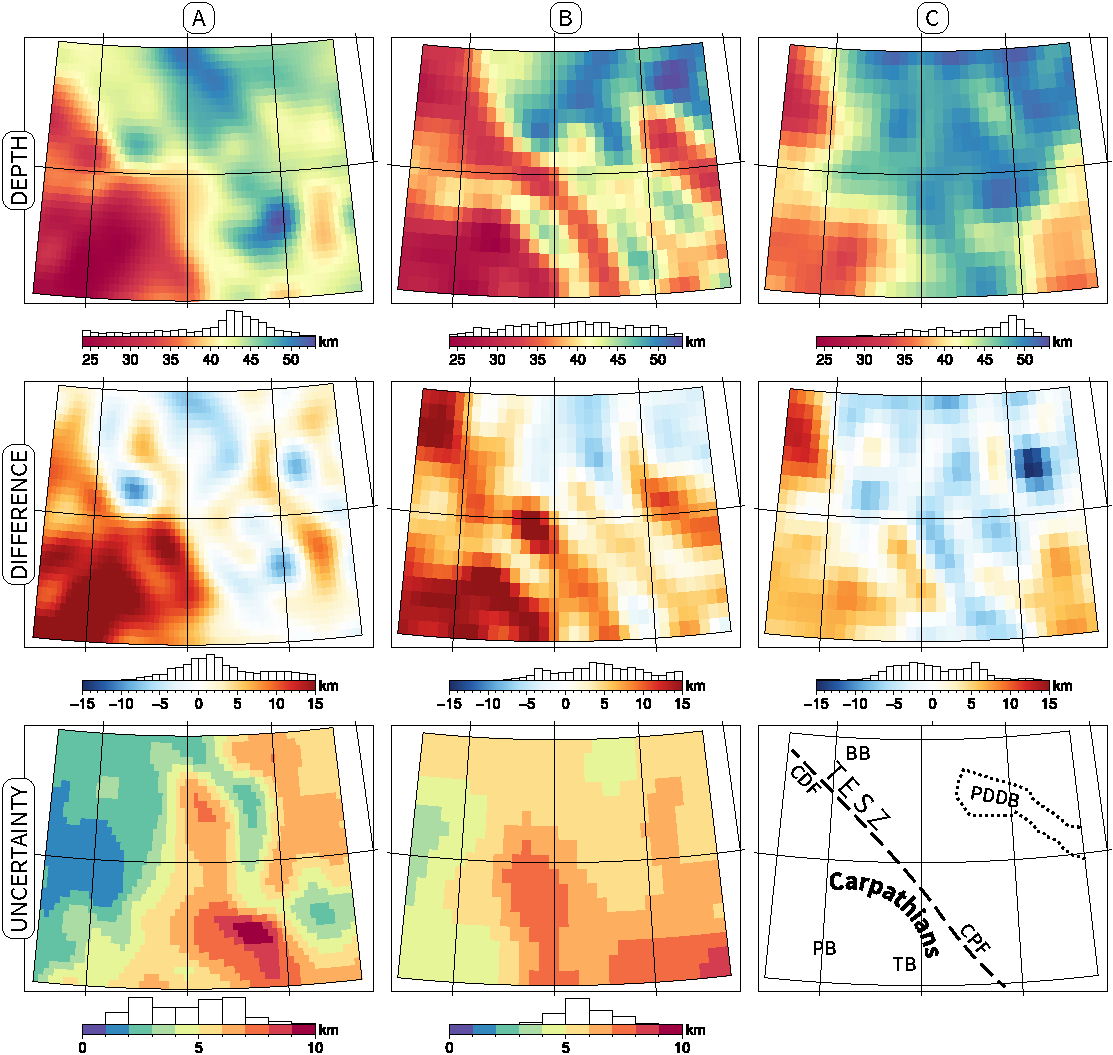
\includegraphics[width=1.2\textwidth]{./0400/MohoComp8.pdf}}
	\end{adjustbox}
	\caption[Comparisons of inverted Moho with three selected crustal models.]{Comparisons with three selected crustal models: \textbf{A)}~European Moho depth by \textcite{Grad2009}, \textbf{B)}~GEMMA GOCE-based global Moho by \textcite{Reguzzoni2015}, \textbf{C)}~{LITHO1.0} global surface-wave-dispersion model by \textcite{Pasyanos2014}.
	First row: Moho depths. Second row: differences, expressed as the inverted depth estimate minus the compared Moho. Third row: uncertainty estimates (not available for {LITHO1.0} depths).
	Lower-right corner: geological features, see Fig.~\ref{fig:INVMoho}.}
	\label{fig:MohoComparisons}
\end{figure}

The Moho depth by \textcite{Grad2009} is the result of a large compilation of data from different methods (seismic reflection and refraction, receiver functions, tomography, joint seismic--gravity inversion), which where harmonised using relative weights.
The model is accompanied by an uncertainty map, obtained from error estimates provided with data or from method-dependent assumptions, when the former were not available.
It is the highest resolution model among these three.

The model by \textcite{Reguzzoni2015}, a global estimate of crustal thickness (and associated uncertainty), is based on data from GOCE, albeit with a different strategy from the one used here, including a novel inversion algorithm.
It is by design highly independent from seismic data (`weakly constrained'), requiring only at least $M+1$ a-priori Moho depths for an Earth divided in $M$ geological provinces.

I have already mentioned and utilised the {LITHO1.0} \parencite{Pasyanos2014} model in this chapter procedure: in the gravity reduction phase to compute a global crustal root effect (`isostatic effect') and in the inversion, where it provided the reference depth (average Moho depth in the study area) and the starting $\Delta \rho$ map.
For these reasons, care must be taken in interpreting the comparison: e.g. the average difference is almost zero due to the chosen average reference depth.

I performed each comparison by downsampling the higher resolution grid to the lower resolution one, between the model obtained in this work and the compared one.
Therefore, the Moho by \textcite{Grad2009}, which is provided on a \SI{0.1}{\degree}~grid, was downsampled to my \SI{0.25}{\degree}~grid; the Moho by \textcite{Reguzzoni2015}, provided on a \SI{0.5}{\degree}~grid was left as is and I downsampled my Moho to \SI{0.5}{\degree}.
The comparison with LITHO1.0 was also performed on a \SI{0.5}{\degree}~grid, due to the non-rectangular tessellation of its original \num{1}~arc-degree spaced global grid.

I summarise the difference range, mean, median, and standard deviation in Tab.~\ref{tab:MohoCompStats}.
The mean difference is directly controlled by the inversion reference depth parameter.
It is positive (i.e. my inverted Moho is deeper) for both \textcite{Grad2009} and \textcite{Reguzzoni2015} models, by 3.7 and 5.0~\si{\kilo \metre} respectively.
This partly explains the consistently positive difference over the areas of thin crust.
The distribution of differences against the three models is never symmetric: the difference between mean and median indicates a positive skew for \textcite{Grad2009} and \textcite{Reguzzoni2015} and a negative skew against the Moho of \textcite{Pasyanos2014}.

\begin{table}
    \caption[Statistics of differences between the Moho depth estimate and the three benchmarks.]{Statistics of differences between the inverted Moho depth estimate and the three benchmarks. This chapter estimate minus the compared Moho depth, expressed in \si{\kilo \metre}.}
    \begin{adjustbox}{center}
    \begingroup\setlength{\fboxsep}{0pt}
    \colorbox{tablebackground}{%
	\begin{tabular}{lrrrrr}
		\toprule
		 \textbf{Crustal model} & \textbf{Min} & \textbf{Max} & \textbf{Mean} & \textbf{Median} & \textbf{St. Dev.} \\
		\midrule
		\textbf{A)}~\textcite{Grad2009} & -10.1 & 18.3 & 3.7 & 2.4 & 6.2 \\
		\textbf{B)}~\textcite{Reguzzoni2015} & -7.7 & 17.4 & 5.0 & 4.7 & 5.7 \\
		\textbf{C)}~\textcite{Pasyanos2014} & -14.6 & 13.1 & 0.1 & 0.6 & 4.9 \\
		\bottomrule
    \end{tabular}
    }\endgroup
    \end{adjustbox}
	\label{tab:MohoCompStats}
\end{table}

In terms of geological structures, the Moho depth I obtained uniformly under-estimates the crustal thinning under the Pannonian basin: in the three compared models it reaches a minimum thickness ranging from 25 to 35~\si{\kilo \metre}, while mine stops at 39~\si{\kilo \metre}.
Such a discrepancy may be explained by an insufficient correction for the sedimentary infill (which would require an even less compacted depth-density model, as discussed before) or by the complex Moho structure in extensional settings \parencite[e.g. due to underplating, see][]{OReilly2013}, which is resolved differently by seismic methods.

The thickened root of the Carpathians is not resolved in the Moho by \textcite{Grad2009}, while it is present in my model and in the ones by \textcite{Reguzzoni2015} and \textcite{Pasyanos2014}.
Its absence in the seismic model could be an artefact of locally poor coverage, a strong point for adopting gravity-derived models even in relatively well-surveyed areas.

I observe a thin NW-SE lineament, from the centre of the study area towards the lower half, in the GEMMA model (\textbf{B}), which is not resolved by the other models.
It is also resolved by my model, and corresponds to a similar lineament in the GOCE data, then enhanced by the sediment correction.
There is a 5 to 10~\si{\kilo \metre} positive misfit between GEMMA and my model, along this lineament.
I speculate it may be originated by the different sediment reduction models, which the authors also applied before inversion.
A thinner crust may result from a larger estimate (in thickness and/or in density) of the effect of the infill of the Carpathians Foredeep.

The misfits are uniformly less over the NE portion of the study area, roughly corresponding to the Russian Platform.
The sensibly thinner crust of the Pripyat-Dnieper-Donets rift is resolved only by the GEMMA model, while it is fainter in the Moho by \textcite{Grad2009}.
The thermal model also resolves that, albeit with the aforementioned underestimation of thinning.
The discrepancy with {GEMMA} can be attributed to their use of geological provinces, through a variable density scale factor for each one. Such a strategy allows to accommodate the sharp differences in Moho contrast of different tectonic regimes, albeit with the added issues of depending on surface data.

Some small-scale Moho undulations in the Russian Platform are resolved by the Moho obtained here and the first two compared models, albeit with different magnitude.
They are not present in the {LITHO1.0} Moho and are the source of the large localised negative misfits (up to -15~\si{\kilo \metre}).
The absence of such small features (about 1~arc-degree across) can be attributed to the lower resolution of {LITHO1.0}.

The misfit with the other models arises due to the unaccounted density variations throughout the crust, which bias the inversion results, and from density variations in the mantle that I am not separating from the crustal contribution.
The former, the intra-crustal masses, can be partly addressed with data integration, where available: it is the case of the sediment stripping reduction I computed and applied.
This can prevent some of the larger systematic errors, such as estimating a thick crust to fit the negative anomaly caused by the low-density infill of a basin.
Still, the choice of a-priori parameters, such as a general compaction model, does not take into account the large variance of geological heterogeneity.
This can range from different compaction curves due to different basin histories \textcite{allen2013basin}, to salt structures (which do not follow ordinary depth-dependence curves), to circumstances which would require more detailed models (e.g uplifted and eroded sedimentary formations, resulting in outcropping rocks with negligible porosity).
% QUI PROVE CON DIVERSE CURVE COMPATTAZIONE

The latter, the `mantle effect', cannot be reliably separated by spectral means (e.g. by truncating the lowest spherical harmonic degrees of the GGM), since large near-surface structures and mantle contributions often overlap \parencite{Kaban2004}.
A viable option is computing a density distribution from a mantle model of velocity anomalies \parencite[e.g. ][]{Kuhn2005}, which is the strategy adopted by \textcite{Reguzzoni2015}, who used the GyPSuM model \parencite{Simmons2010}.
I have chosen to not perform such kind of reduction, owing to the additional uncertainties involved and on its temperature dependency.
I have taken into account only the lateral variation of the lithospheric mantle density, which I included in the `isostatic correction' to calculate a global Moho contrast (see Eq.~\ref{eq:RhoContrast} and~\ref{eq:ACY400}).

\section{Thermal modelling results}
\label{s:Appl:DiscTherm}

\subsection{Heat flow data}
\label{ss:Appl:DiscTherm:HF}

\begin{figure}
	\begin{adjustbox}{center}
	\fbox{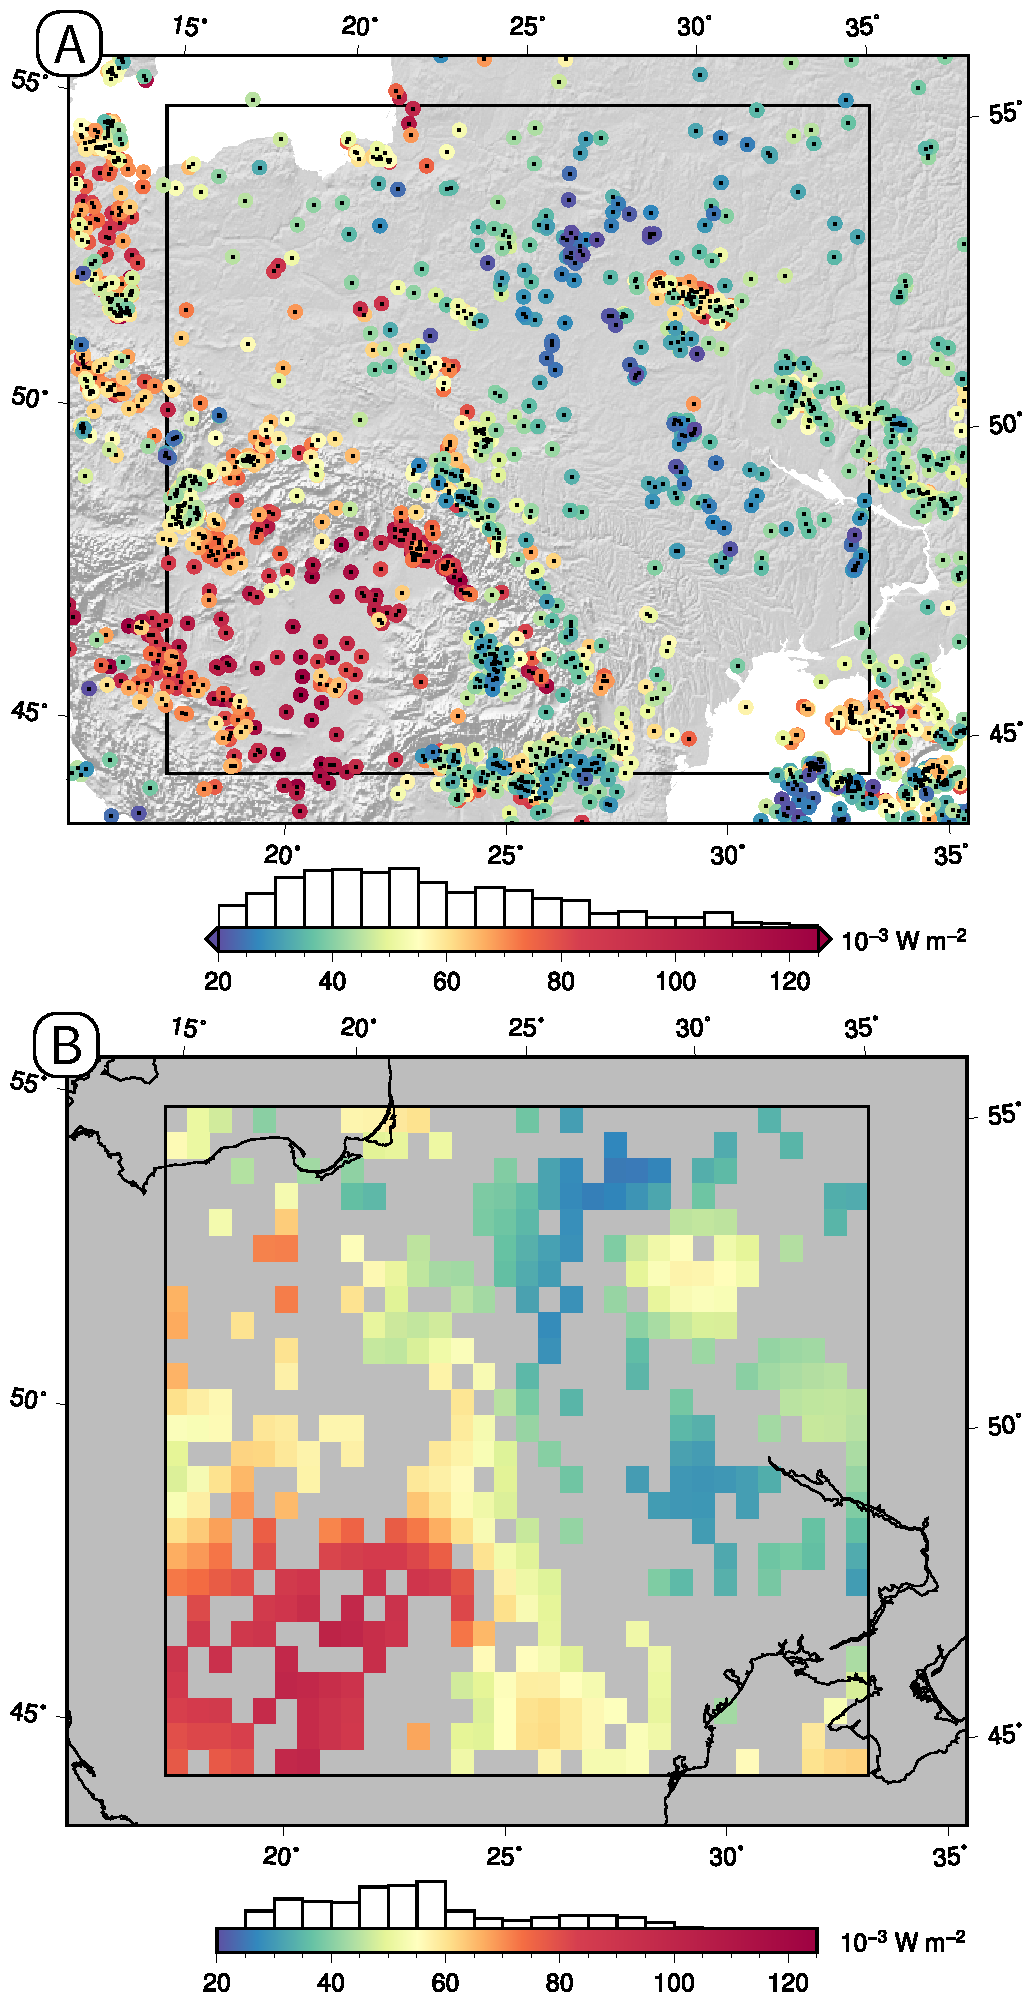
\includegraphics[width=0.725\textwidth]{./0400/HFmerged.pdf}}
	\end{adjustbox}
	\caption[Surface heat flow, sample points and block-median processed.]{\textbf{A)}: surface heat flow sample points, from \textcite{globalHF}. The histogram counts only the points inside the study area (inner rectangle). Note that there is considerable overlap in the most sampled spots, this is partly conveyed by the overlayed black dots. \textbf{B)}: the processed surface heat flow grid, after block-median and raised cosine low-pass filtering of the sample points.}
	\label{fig:HFdata}
\end{figure}

The filtered and gridded surface heat flow measurements (shown in Fig.~\ref{fig:HFdata}, B) highlight two distinct thermal regimes, which after filtering are distributed in a 80~\si{\milli \watt \per \square \metre} wide range.
There is a south-west to north-east gradient across the TESZ lineament, albeit complicated by small wavelength variations.
The cells with highest values are clustered in the Pannonian Basin, where considerable variance is observed (70 to 105~\si{\milli \watt \per \square \metre}).
The lower-than-average heat flow cells in the Russian Platform include a superimposed local maximum (54.9~\si{\milli \watt \per \square \metre}) coinciding with part of the Pripyat-Dnieper-Donets rift.
Note that this also coincides with a spot of thin crust (up to 35~\si{\kilo \metre}).

Block-median gridding and low pass filtering decreased the standard deviation from 23.6 to 17.81~\si{\milli \watt \per \square \metre}.
The average of the raw samples is 57.1~\si{\milli \watt \per \square \metre}, it becomes 54.8~\si{\milli \watt \per \square \metre} after processing.
Processed surface heat flow in the grid cells range from 26.2 to 98.0~\si{\milli \watt \per \square \metre}.
For comparison, the global average continental surface heat flow is estimated at 64~\si{\milli \watt \per \square \metre}, as concordantly found with different strategies by \textcite{Davies2010} and \textcite{Pollack1993}.
No-data cells cover 58\% of the study area.

\subsection{Iterative forward modelling output}
\label{ss:Appl:DiscTherm:FWD}

\begin{figure}
	\begin{adjustbox}{center}
	\fbox{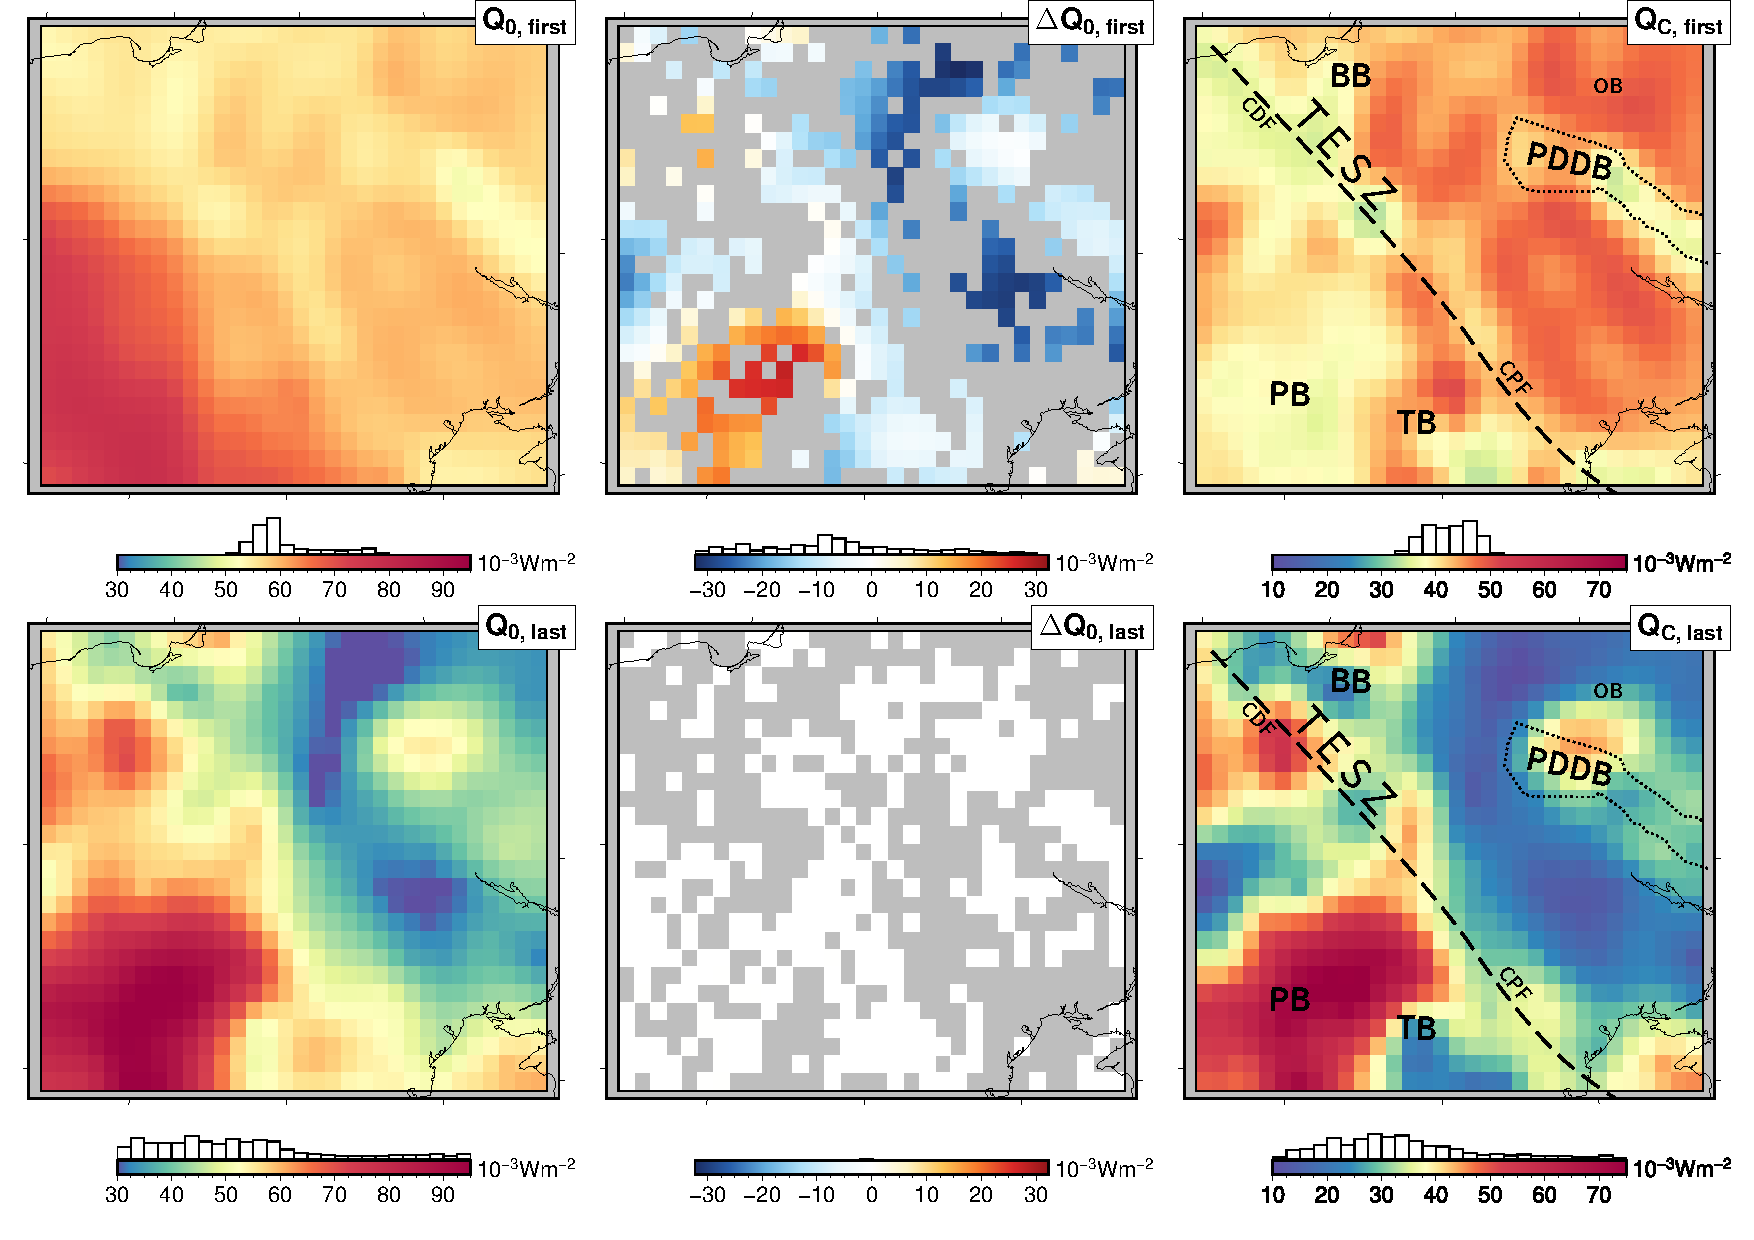
\includegraphics[width=1.35\textwidth]{./0400/Q1arrays.pdf}}
	\end{adjustbox}
	\caption[Results of the iterative fit on the thermal model, in terms of surface heat flow.]{Results of the iterative fit on the thermal model, in terms of surface heat flow. \textbf{Top row:}~first iteration, only a-priori crustal heat production. \textbf{Bottom row:}~last iteration. \textbf{Left column:}~surface heat flow; \textbf{middle column:}~misfit between heat flow measurements and forward-modelled heat flow; \textbf{right column:}~crustal (radiogenic) component of surface heat flow.}
	\label{fig:Qresults}
\end{figure}

The top row of Fig.~\ref{fig:Qresults} shows the output after the first iteration of the thermal model (`first guess', as described in section~\ref{ss:Appl:ThermRHP}).
The surface heat flow misfit between the forward model (left map, $Q_{0,\mathrm{first}}$) and the measurements is shown in the central map ($\Delta Q_{0,\mathrm{first}}$).
The average misfit is -7.5~\si{\milli \watt \per \square \metre}, with a standard deviation of 13.7~\si{\milli \watt \per \square \metre}.
Those results indicate how the crust thickness alone can explain only a limited part of the variance in the observed heat flow, confirming a common finding \parencite[e.g. ][]{Jaupart2016}.
The first-guess was run with a laterally uniform crustal heat production per unit of volume of \SI{1.04}{\micro \watt \per \cubic \metre}, partitioned between the upper crust (\SI{1.74}{\micro \watt \per \cubic \metre}) and the lower crust (\SI{0.37}{\micro \watt \per \cubic \metre}).
The right map ($Q_{0,\mathrm{first}}$) shows the crustal heat flow contribution, expressed as the difference between the heat flow at the base of the sediments layer and the heat flow at the crust-mantle boundary. 
At this stage, it is directly proportional to crustal thickness.

\begin{figure}
	\begin{adjustbox}{center}
	\fbox{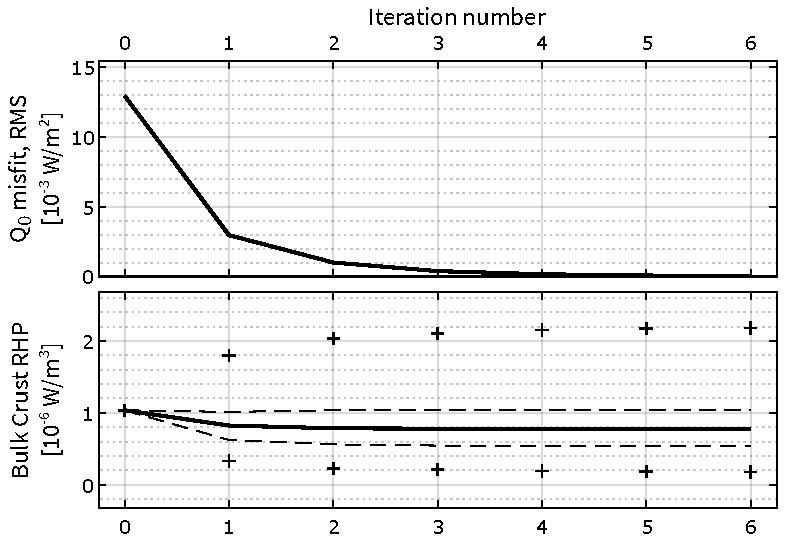
\includegraphics[width=0.75\textwidth]{./0400/RMS_Afit_2.pdf}}
	\end{adjustbox}
	\caption[Behaviour of the subsequent substitution fitting procedure in 6 iterations, plus the first guess.]{Behaviour of the subsequent substitution fitting procedure in 6 iterations, plus the first guess. RMS surface heat flow misfit (\textbf{top}) and radiogenic heat production in the upper crust (per unit of volume, \textbf{bottom}). The tick line denotes the median, the two dashed lines the first and third quartiles, respectively, the crosses minimum and maximum values.}
	\label{fig:RMSvsITN}
\end{figure}

The bottom row of Fig.~\ref{fig:Qresults} shows the same variables of the first row, at the sixth crustal RHP fitting iteration.
The same colour scale is adopted.
Here practically all the signal in the surface heat flow is modelled, leaving a mean misfit of 0.005~\si{\milli \watt \per \square \metre} (standard deviation 0.038~\si{\milli \watt \per \square \metre}).
The converging behaviour of RMS misfit over the six iterations is shown in the top plot of Fig.~\ref{fig:RMSvsITN}: it decreased from 13.0~\si{\milli \watt \per \square \metre} to 0.03~\si{\milli \watt \per \square \metre}.
The trend of the distribution of fitting heat production is shown in the bottom plot of the same figure.
While the median value of heat production is reduced by of \SI{0.26}{\micro \watt \per \cubic \metre} from start to end, the fitted values are distributed between \num{0.18} to \SI{2.18}{\micro \watt \per \cubic \metre} (minimum to maximum) after the last iteration.
The width of their distribution appears directly connected to the decreasing misfit shown in the top plot.
The map on the right in Fig.~\ref{fig:Aresults} shows the fitted heat production values, for each crustal column.
Their distribution is skewed toward low values, resembling the empirically observed asymmetrical distribution of rock heat production values \parencites{Vila2010}{Artemieva2017granite}{Hasterok2017_ign}, which has been modelled with a log-normal distribution sometimes \parencites[e.g. ][]{Jokinen1999}{Huang2013}.

\begin{figure}
	\begin{adjustbox}{center}
	\fbox{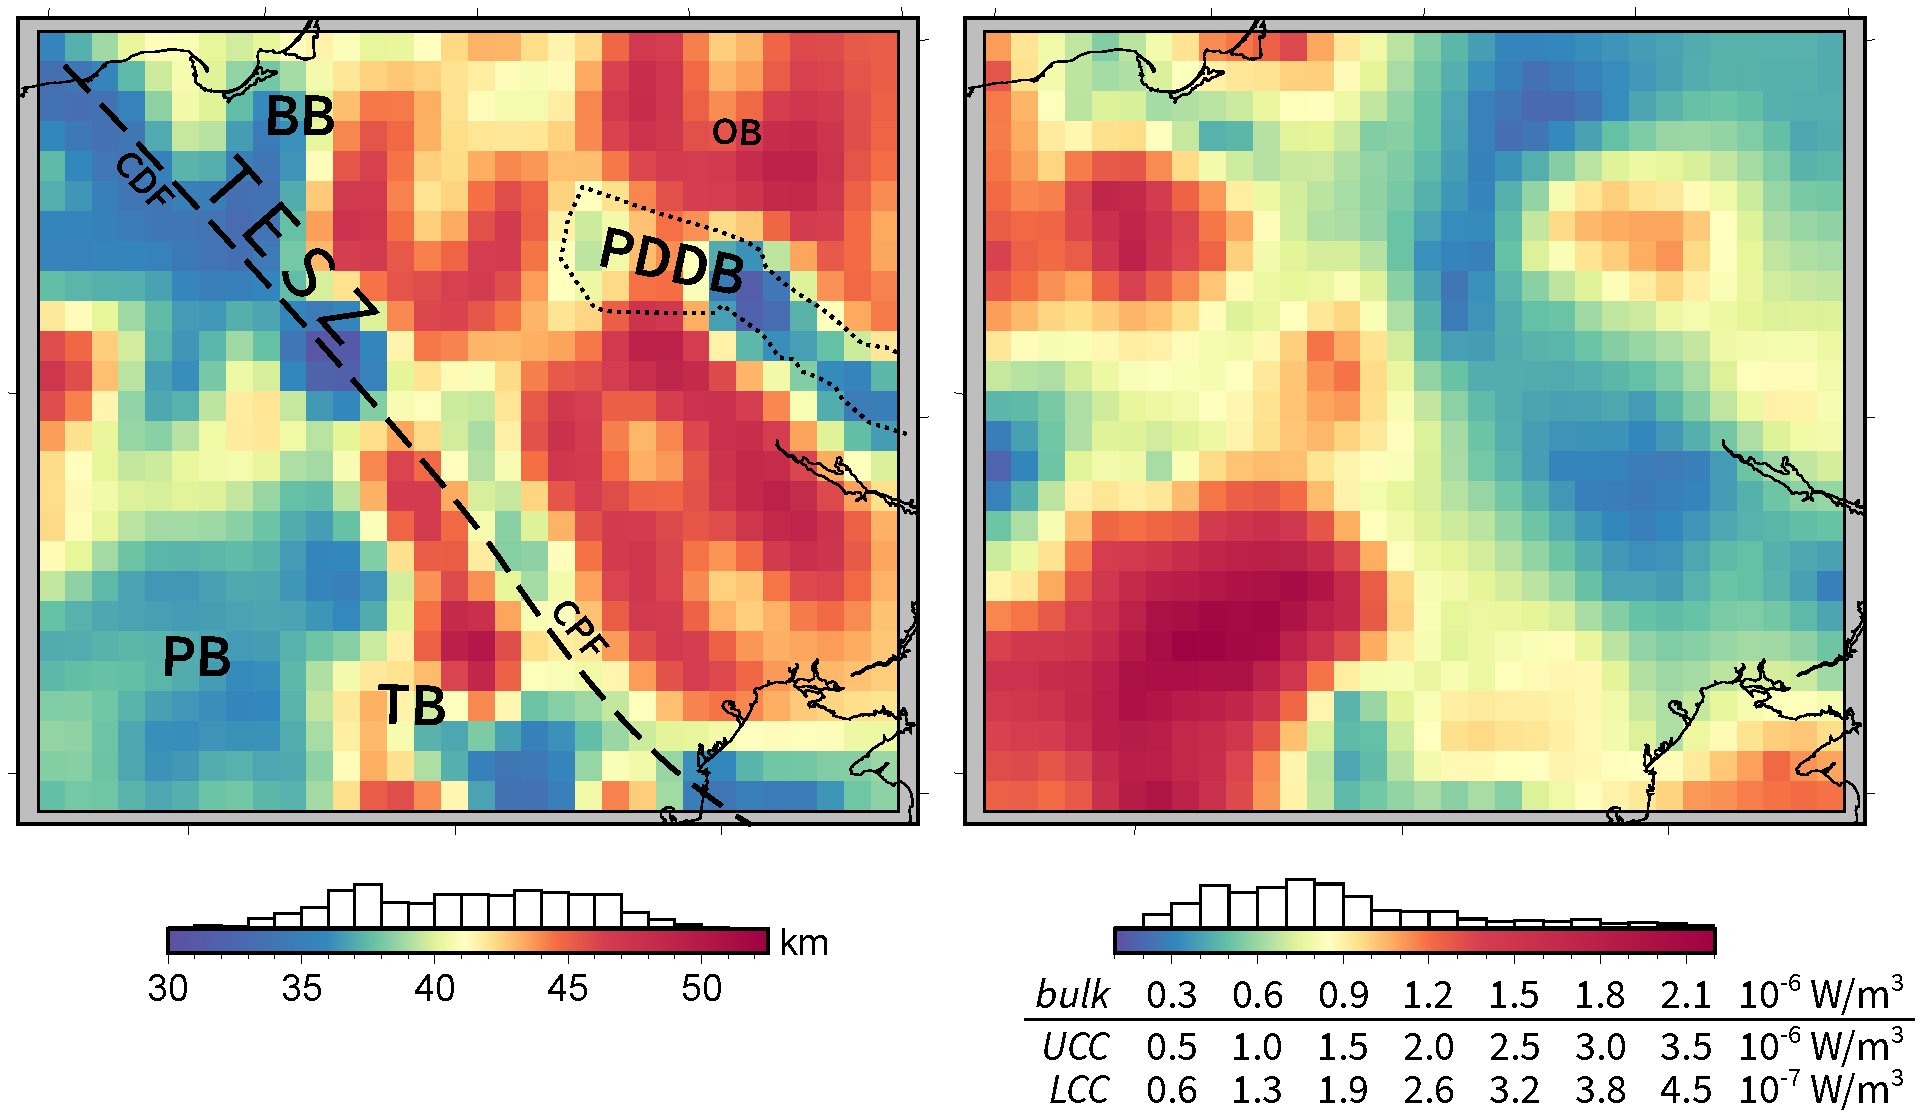
\includegraphics[width=0.9\textwidth]{./0400/ACmerged.pdf}}
	\end{adjustbox}
	\caption[Fitted radiogenic heat production (RHP) in the crystalline crust, per unit of volume.]{Fitted radiogenic heat production (RHP) in the crystalline crust, per unit of volume. \textbf{Left:}~thickness of crystalline crust: Moho depth minus sediment basement depth; \textbf{right:}~RHP: bulk and partitioned to upper and lower crystalline crust (note that the lower crust RHP unit is one order of magnitude smaller). Geographical labels: see Fig.~\ref{fig:INVMoho}.}
	\label{fig:Aresults}
\end{figure}

The spatial distribution of crustal heat production shows a first-order correlation with surface heat flow.
This is a direct consequence of fitting all the variance not arising from the thickness of the crust and lithosphere with heat production, as I have shown before.
Still, deviations from a pure correlation between heat flow and heat production arise from the contribution of crustal thickness, as can be seen by comparing the crustal heat flow contribution, in the right map of Fig.~\ref{fig:Qresults}, against the thickness of the crystalline crust (left map of Fig.~\ref{fig:Aresults}).
I resort to the cross-plots of Fig.~\ref{fig:Qcrossplots} to better show this.

\begin{figure}
	\begin{adjustbox}{center}
	\fbox{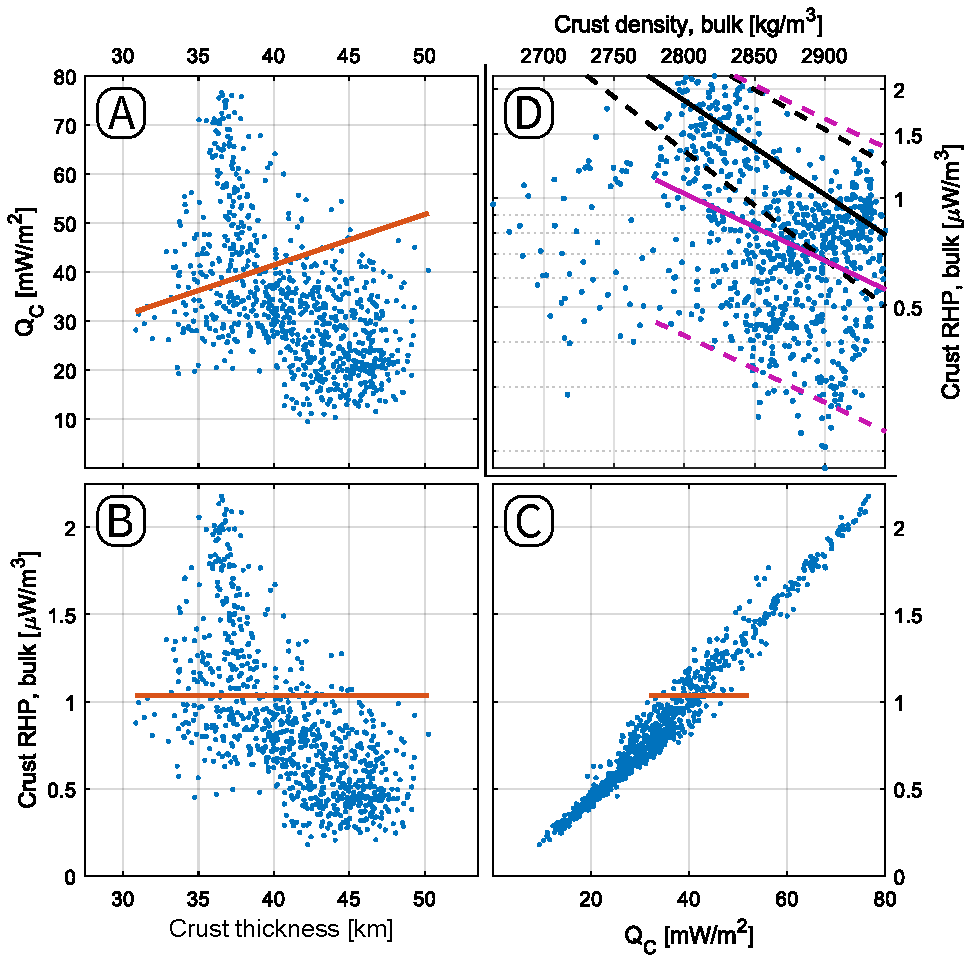
\includegraphics[width=1.2\textwidth]{./0400/crossplots_tight.pdf}}
	\end{adjustbox}
	\caption[Cross plots between thickness of the crystalline crust, RHP of the bulk crystalline crust, crustal component of heat flow, and crust density.]{Cross plots between thickness of the crystalline crust (Moho depth minus basement depth), radioactive heat production (RHP) of the bulk crystalline crust, crustal component of heat flow ($Q_C$), and crust density. The line overlaid on scatter~plots \textbf{A)} to \textbf{C)} represents the first guess, using the a-priori constant RHP.
	Plot \textbf{D)}: bulk density of the crystalline crust plotted against the radioactive heat production (RHP). The density-heat production relationship by \textcite{Hasterok2017_ign} is plotted in black. The fit with this chapter data is plotted in purple. Dashed lines depict upper and lower confidence bounds.}
	\label{fig:Qcrossplots}
\end{figure}

The line overlain to scatter~plots \textbf{A} to \textbf{C} represents the results of the first guess, in a perfect crustal thickness to crustal heat flow relationship, with no lateral variations in RHP.
Two distinct behaviours of departure from the first guess line can be observed: the first, a cluster which has most of its points confined between 35 and 40~\si{\kilo \metre} of thickness, increased its RHP value with respect to the first guess.
It corresponds to those heat flow values found in the extensional basins, as shown in the maps of Fig.~\ref{fig:Qresults}.
The other, which involves the remainder of points, is considerably scattered along a trend of inverse proportionality between crustal thickness and RHP, opposite to the first guess.
This weak negative relationship is a common finding of studies on relationships between heat flow and crustal thickness \parencites{Cermak1993}{Mareschal2013}.

As described before, the RHP fill-in method presented here relies on the interpolation of fitted RHP, which is available in cells where surface heat flow measurements are available, over cells where there are none.
I assumed that $A$, the RHP per unit of volume, is uncorrelated to crustal thickness.
Therefore, the interpolation does not take into account Moho undulations.
As shown in plot \textbf{B)} of the crossplots figure (Fig.~\ref{fig:Qcrossplots}), I observe a negative proportionality between Moho depth and fitted RHP.
This a-posteriori observation suggest that a correlation between the two exist and could be exploited to further constraint the RHP fill-in.
Nevertheless, it should be interpreted with caution.
There is an issue with the attribution of heat flow misfit to crustal or mantle sources, which I address in the next section.

In Fig.~\ref{fig:Qcrossplots}~\textbf{D} I plotted the fitted RHP of this work against the bulk density of LITHO1.0 \parencite{Pasyanos2014} crystalline crust, computed by thickness-weighted averaging of the three crustal layers.
I did so in order to compare my result to the density to heat production relationship provided by \textcite{Hasterok2017_ign}: $\log_{10} A = -0.0027 (\rho - 2700) + 0.53 $ (plotted in black).
In contrast to my indirect estimates, their results are based on geochemical data of more than {100,000} samples.
I perfomed a log-linear fit to the fitted RHP data, obtaining the following relationship, plotted in purple:

\begin{equation}
	\label{eq:RHP_RHO_fit}
	\log_{10} A = -0.0019 (\rho - 2700) + 0.20
\end{equation}
The $2\sigma$ confidence interval of this fit is \num{-0.0022} to \SI{-0.0015}{(log_{10} \micro \watt \per \cubic \metre)(\kilo \gram \per \cubic \metre)^{-1}} for the slope and \num{0.14} to \SI{0.26}{\micro \watt \per \cubic \metre} for the intercept.
$R^2$ is \num{0.1274}.
I excluded the nodes with a bulk density lower than 2780~\si{\kilo \gram \per \cubic \metre}, since they are underrepresented in the study area (less than 7\% of total nodes, clustered in the southeast corner).
A negative relationship between density and RHP can be observed --it can be attributed to the increased content in heat producing elements in less dense, more felsic rocks \parencite{Hasterok2017_ign}.
The two fits, albeit different, overlap in their uncertainty interval.
A version of the scatter~plots of Fig.~\ref{fig:Qcrossplots} in which a colour scale is used to depict each node density, and a map of the bulk density of the crystalline crust in the study area are provided in the appendix (section~\ref{s:ApplSup:Rel}, Fig.~\ref{fig:RhoRHP}).

I also compared this fitted-RHP estimate with the V\textsubscript{P} to heat production conversion provided in \textcite{Hasterok2017_ign}, using their log-linear relationship for the continental crust ($\log_{10} A = -0.70 (V_{P} - 6) + 0.48$).
Due to the relationship between density and V\textsubscript{P}, the pattern is similar to what I just discussed concerning density. A similar trend of negative correlation is observed, with the the results presented here shifted toward lower values: $\log_{10} A = -0.56 (V_{P} - 6) + 0.19$.
The geochemistry-based linear fit and the one that I obtained by linear regression on the inverted data again overlap in their $2\sigma$ uncertainty interval.
The V\textsubscript{P}-converted RHP is consistently higher than my estimate over the whole area (mean \SI[retain-explicit-plus]{+0.42}{\micro \watt \per \cubic \metre}, with a local maximum of \SI[retain-explicit-plus]{+1.84}{\micro \watt \per \cubic \metre} in the southeastern corner of the area (local cluster with V\textsubscript{P} less than \SI{6.2}{\kilo \metre \per \second}.
The inverted RHP estimate (i.e.~constrained by crustal thickness, surface heat flow and thermal modelling) is higher than the $V\textsubscript{P}$-converted one only in the Pannonian Basin (difference of up to \SI{-0.59}{\micro \watt \per \cubic \metre}).
A figure with a scatter plot of V\textsubscript{P} and RHP, accompanying maps and further details on the log-linear fit to my data are provided in the appendix material (section~\ref{s:ApplSup:Rel}).

\subsection{Partitioning of heat flow between crust and mantle sources}
\label{ss:Appl:DiscTherm:Partition}

\begin{figure}
	\begin{adjustbox}{center}
	\fbox{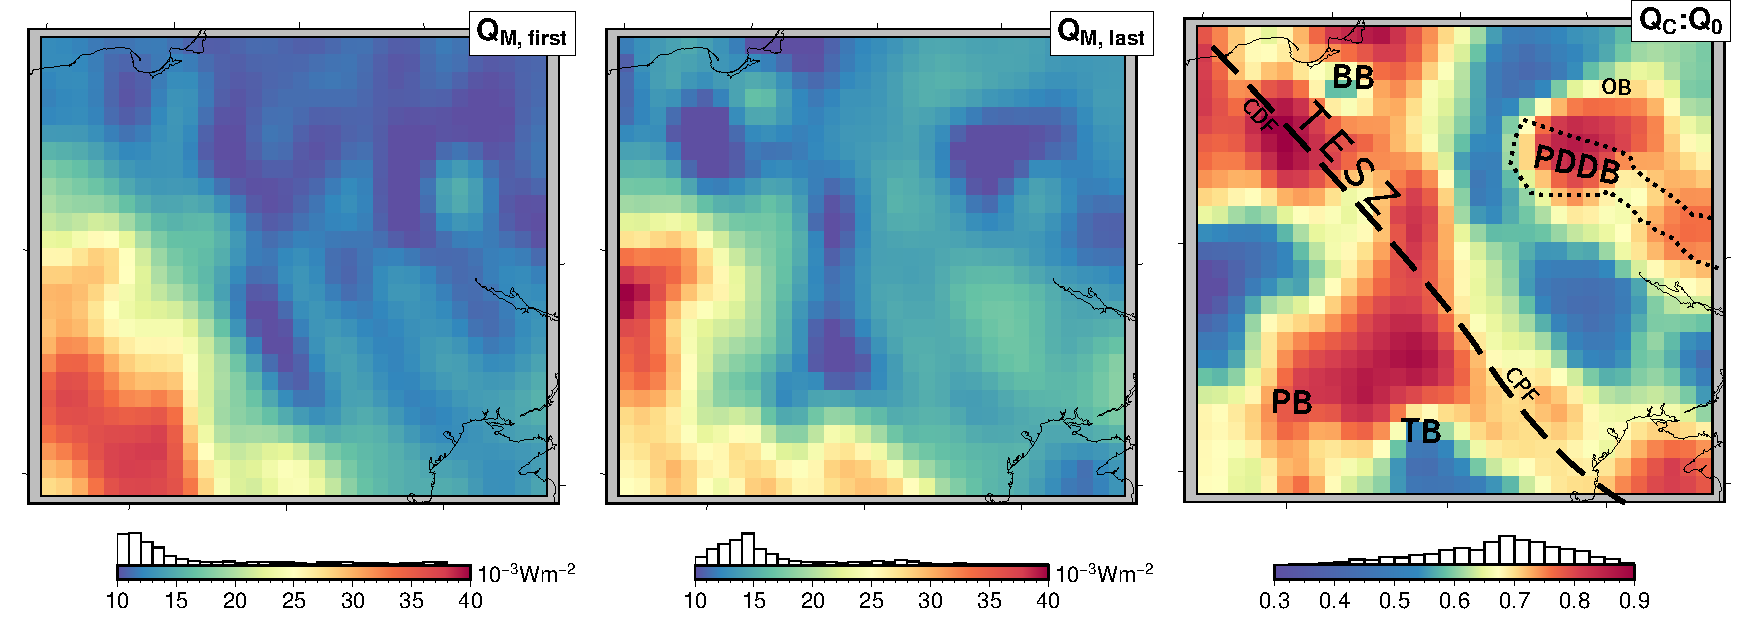
\includegraphics[width=1.35\textwidth]{./0400/Q3arrays_labels.pdf}}
	\end{adjustbox}
	\caption[Basal heat flow at the crust-mantle boundary.]{Basal heat flow ($Q_M$), at the crust-mantle boundary. \textbf{Left:}~$Q_M$ at the first iteration (a-priori parameters); \textbf{middle:}~$Q_M$ at the last iteration; \textbf{right:}~partition coefficient, expressed as the ratio between crustal component of heat flow ($Q_C$) and the total surface heat flow ($Q_0$), at the last iteration.}
	\label{fig:QM}
\end{figure}

Since the strategy presented here is based on the assumption that all the surface heat flow misfit can be attributed to omitted crustal heat production, I analyse what this implies for the partition between the crustal contribution ($Q_C$) and the basal, mantle-borne, heat flow component ($Q_M$, Fig.~\ref{fig:QM}).
This has also been referred to as `partition coefficient'. \textcite{Hasterok2016} expressed it as the basal to surface heat flow ratio.
Here I have adopted the crustal to surface heat flow ratio ($Q_C:Q_0$) as a partition metric.
I also define the basal heat flow as the heat flow through the crust-mantle boundary, since I am including lateral variations of heat production in the lower crust.
A larger ratio indicates a thermal regime dominated by crustal heat production.

The top plot of Fig.~\ref{fig:QMvsITN} shows how this partition varies through the iterations: the largest variation occurs between the first guess (iteration zero) and iteration one, where the median $Q_C:Q_0$ drops by $8.6$ points percent.
No significant variation in the median occurs between iteration 1 and 6.
The range between the extreme values (denoted with `plus' signs) and the inter-quartile range (between the first and thirt quartile, plotted with dashed lines) widen, with a trend that flattens after iteration 4.

\begin{figure}
	\begin{adjustbox}{center}
	\fbox{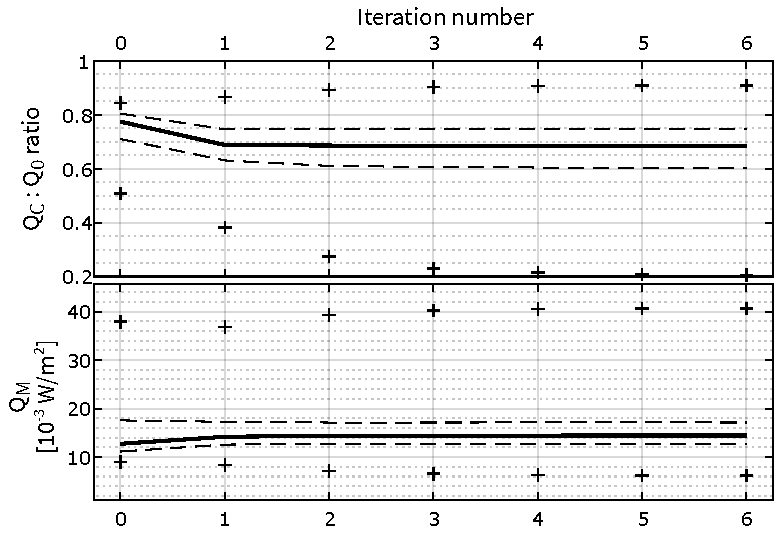
\includegraphics[width=0.75\textwidth]{./0400/QMR_Afit_2.pdf}}
	\end{adjustbox}
	\caption[Partition ratio and heat flow at the crust-mantle boundary.]{\textbf{Top:}~ratio of the crustal heat flow component ($Q_C$) against the surface heat flow ($Q_0$), as shown in the right map of Fig~\ref{fig:QM}. \textbf{Bottom:}~heat flow at the crust-mantle boundary ($Q_M$). The distribution statistics at each iteration are plotted with different symbols. For a legend, refer to the caption of Fig.~\ref{fig:RMSvsITN}.}
	\label{fig:QMvsITN}
\end{figure}

The bottom plot of Fig.~\ref{fig:QMvsITN} represents the trend of $Q_M$, which appears anticorrelated with the ${Q_C:Q_0}$ ratio.
This behaviour stems from the suppression of basal heat flow that is observed for an increase in crustal heat production.
Basal heat flow, for a fixed radiogenic $Q_C$, would be only controlled by the depth of the LAB-isotherm and the series thermal resistance of the LAB-to-surface path.
A steeper geotherm (i.e. a warmer crust) decreases the thermal conductivity of the crust \parencite[see Eq.~\ref{eq:kTzChap86} here and ][]{Chapman1986}, resulting in a lower $Q_M$ for the same LAB depth.
In addition, thermal refraction is observed around an hotter crustal body, since the steepest temperature path is not along vertical any more (for synthetic examples, see sections~2 and 3 provided in the Supplementary Material).

This implies that whenever a positive misfit in $Q_0$ (i.e. not enough crustal heat production) is fitted for, $Q_M$ in the same model column will decrease in the subsequent forward modelling iteration.
This will result in a positive misfit again, albeit smaller.
The opposite happens for a negative misfit, whenever the forward modelled surface heat flow is higher than the observed.

Plotting the evolution of $Q_M$ on a map (Fig.~\ref{fig:QM}) provides further information on the spatial distribution of this variation, and its relationship with geology.
The left map (iteration zero, labelled $Q_{M,first}$) shows a thermal regime which is strongly controlled by the LAB morphology (Fig.~\ref{fig:LAB}): the warmer and thinner south-west European Phanerozoic lithosphere and the colder, thicker, platform across the suture zone.
The local effect of overlying crustal structures can be already seen, superimposed.
The middle map (sixth iteration, labelled $Q_{M,last}$) highlights where the starting situation was conserved and where it was reversed.
By comparing it with the iteration zero misfit map of Fig.~\ref{fig:Qresults} (middle top row), it can be seen how the strongest transitions from high to low $Q_M$ and vice versa are clustered on the areas of largest misfit.
This reversal can be thus attributed to the inverse dependence mechanism described before.

Overall, the local extremes in $Q_C$, and their accompanying minimums in $Q_M$ should be interpreted with caution: comparison with the geological settings suggests that they may be a symptom of over-estimation of the $Q_C:Q_0$ ratio, when the source of increased heat flow should be attributed to others factors, instead.
This is most evident in the Pannonian Basin and, to a lesser extent, in the Pripyat-Dnieper-Donets basin and in the Caledonides Foredeep.
This can be attributed to the persistence of non-stationary heat transport.
The Pannonian Basin is expected to have significant departures from thermal equilibrium.
I obtain a rough order of magnitude estimate with the end of its rifting phase, around 14~Ma \parencite{Horvath2015} and the characteristic time scale for reaching quasi-steady state conditions, as defined in \parencite{stuwe2007geodynamics}.
The $l^2 / 2\kappa$ rule, as provided in \textcite{stuwe2007geodynamics}, with $l$ length scale and $\kappa$ thermal diffusivity, results in a time scale for reaching equilibrium on the order of $10^2$~My for a $10^8$~m length scale (lithospheric thickness).

Note how spots of localised thinning of the crystalline crust (see Fig.~\ref{fig:Aresults}, left) result in enhanced $Q_m$, persisting through the iterations: this is the result of higher effective thermal conductivity of the LAB-to-surface path, since thermal conductivity is lower in the crust than in the lithospheric mantle.
It is a phenomenon similar to the blanketing and chimney effects observed by \textcite{Przybycin2015} for variations in sediment thickness.

\subsection{AA' section}
\label{ss:Appl:DiscTherm:Section}

In Fig.~\ref{fig:AAsection} a 2D~slice under the AA' profile is plotted (shown in the geological setting map, Fig.~\ref{fig:geosetting}).
It encompasses the different thermal regimes encountered across the study area, which are dominated by the aforementioned southwest-to-northeast transition to older and colder lithosphere.

\begin{figure}
	\begin{adjustbox}{center}
	\fbox{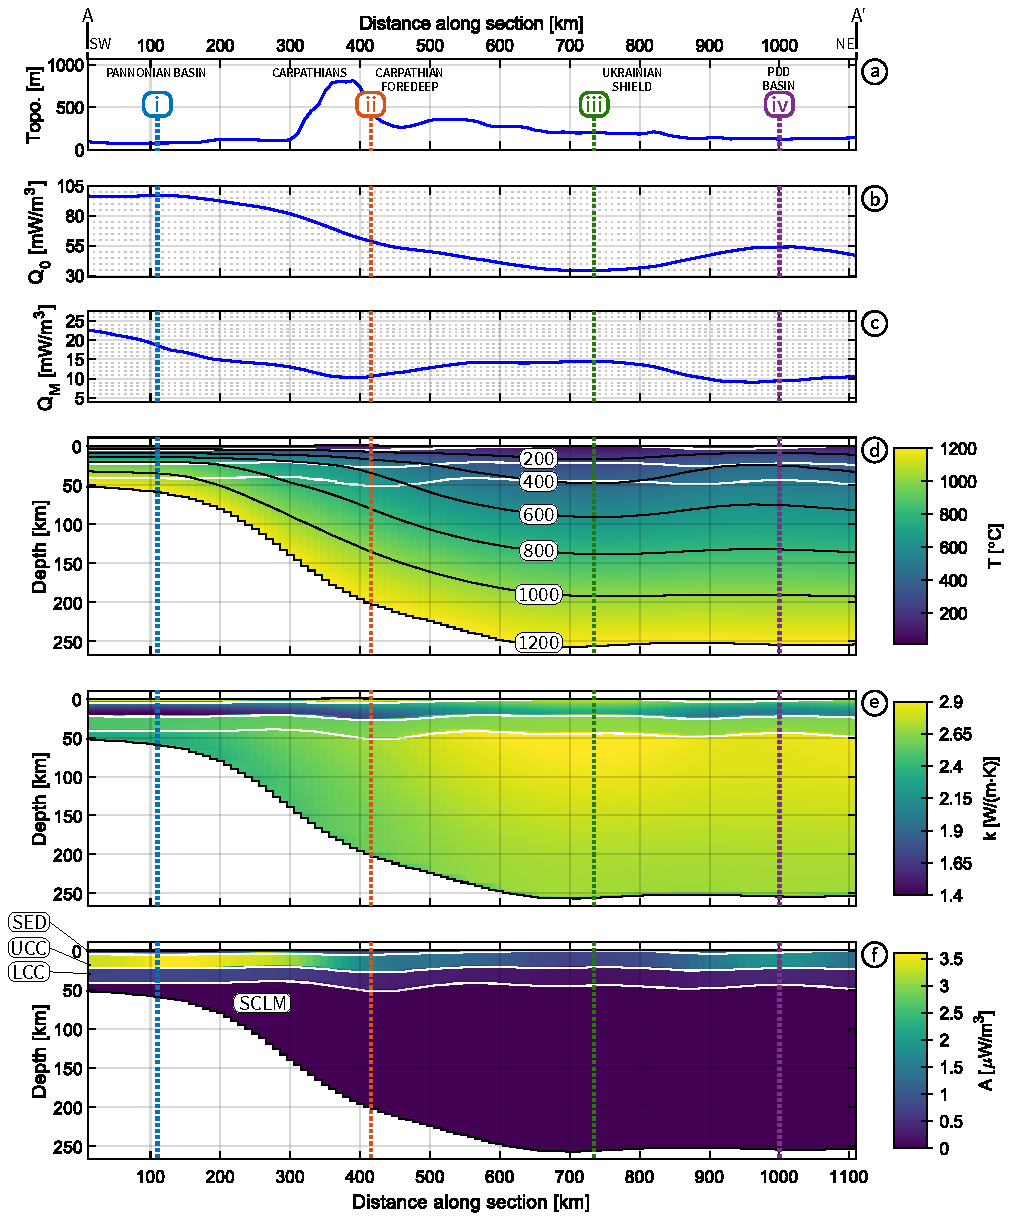
\includegraphics[width=1.1\textwidth]{./0400/sectionAA.pdf}}
	\end{adjustbox}
	\caption[Thermal model section AA'.]{Thermal model section \textit{AA'} (extents are shown in Fig.~\ref{fig:geosetting}).
	\textbf{a)}~topographic profile.
	\textbf{b)}~$Q_0$, surface heat flow profile
	\textbf{c)}~$Q_M$, Moho heat flow profile.
	\textbf{d)}~temperature slice.
	\textbf{e)}~thermal conductivity slice.
	\textbf{f)}~radiogenic heat production slice.
	Layer boundaries are shown in white and labelled on the left side of the bottom slice.
	Abbrevations: \textbf{PDD}~Pripyat-Dnieper-Donets basin, \textbf{SED}~sediments, \textbf{UCC}~upper crystalline crust, \textbf{LCC}~lower crystalline crust, \textbf{SCLM}~sub-continental lithospheric mantle.}
	\label{fig:AAsection}
\end{figure}

The effect of the crust, including sediments, is superimposed on the signal from lithospheric thickness.
The thermal conductivity section shows the effect of thermal dependence of $k$ and its role in controlling $Q_M$.
The portions of hotter crust and lithosphere (e.g. the SW portion of the section) are accompanied by a strong reduction in $k$ in the upper crust and in the lithospheric mantle.
The lower crust sees the concurrent effect of the temperature-driven decrease of $k$ ---a dependence which is an order of magnitude weaker than in the upper crust, in the adopted \textcite{Chapman1986} model--- and increase of $k$ due to rising pressure.
The total effect is a slight increase in conductivity with depth, in concordance with the data shown in \textcite{Chapman1986}.
This depth-wise trend is clearly represented for 4 sample columns in the middle plot of Fig.~\ref{fig:AAsectionCols}.
I must emphasize how this outcome is strongly dependent on the reliability of the assumed temperature-conductivity relationships, therefore it should be interpreted only in conjunction with other temperature proxies (e.g. xenoliths, Curie depth, effective elastic thickness).

\begin{figure}
	\begin{adjustbox}{center}
	\fbox{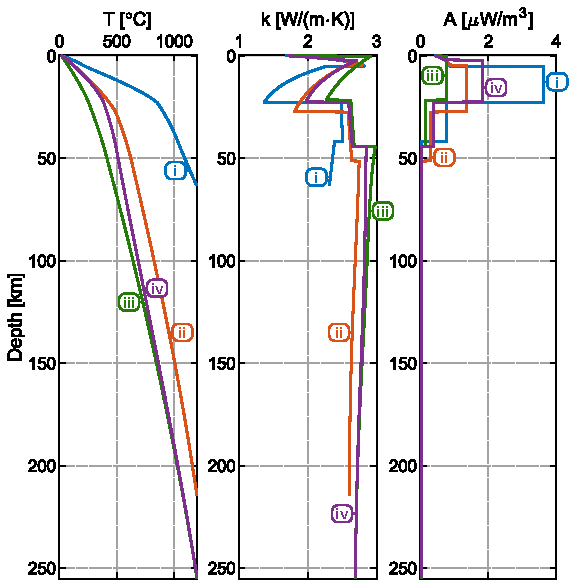
\includegraphics[width=\textwidth]{./0400/sectionAA_cols.pdf}}
	\end{adjustbox}
	\caption[Plots of temperature, thermal conductivity and heat production in four columns of section AA'.]{Plots of temperature, thermal conductivity and heat production in four columns of section AA' (Fig.~\ref{fig:AAsection}). Colours and roman numerals refer to the corresponding labels in the section figure.
	\textbf{i)}~Pannonian Basin, 
	\textbf{ii)}~Carpathians, 
	\textbf{iii)}~Ukrainian Shield, 
	\textbf{iv)}~Pripyat-Dnieper-Donets Basin.}
	\label{fig:AAsectionCols}
\end{figure}

Thick sedimentary covers (Pannonian basin, Carpathians foredeep: columns \textit{i} and \textit{ii}, plotted in blue and orange respectively) further contribute in the reduction of the total thermal conductivity of the lithosphere, attenuating the effect of LAB undulations.
$Q_M$ exhibits a relative maximum across the Ukrainian shield (column \textit{iii}, plotted in green), albeit being over a very thick lithosphere.
There, a combination of thin sedimentary cover, a cold crystalline crust, and a relatively cold lithospheric mantle (note the depression in isotherms in plot \textbf{d}) result in a more conductive lithosphere overall.

\subsection{Sensitivity of the result to crustal thickness}
\label{ss:Appl:DiscTherm:Sens}

In Fig.~\ref{fig:CompCheckMoho} I present the comparison of the results obtained with a flat Moho (44~\si{\kilo \metre}, i.e. the average of the inverted Moho depth estimate) and a synthetic `checkerboard Moho'.
The latter alternates between \num{40} and \SI{48}{\kilo \metre} of thickness, on \num{120}~by~\SI{120}{\kilo \metre} tiles.
I plotted the difference between fitted RHP, basal heat flow, and temperature at \SI{30}{\kilo \metre}.
The difference is expressed as the value obtained with the flat-Moho model minus the value obtained with the checkerboard-Moho one, i.e. positive values indicate larger results in the latter.
As a reference for the alternating pattern, the south-west corner is a thin tile (\SI{40}{\kilo \metre} thick crust).

\begin{figure}
	\begin{adjustbox}{center}
	\fbox{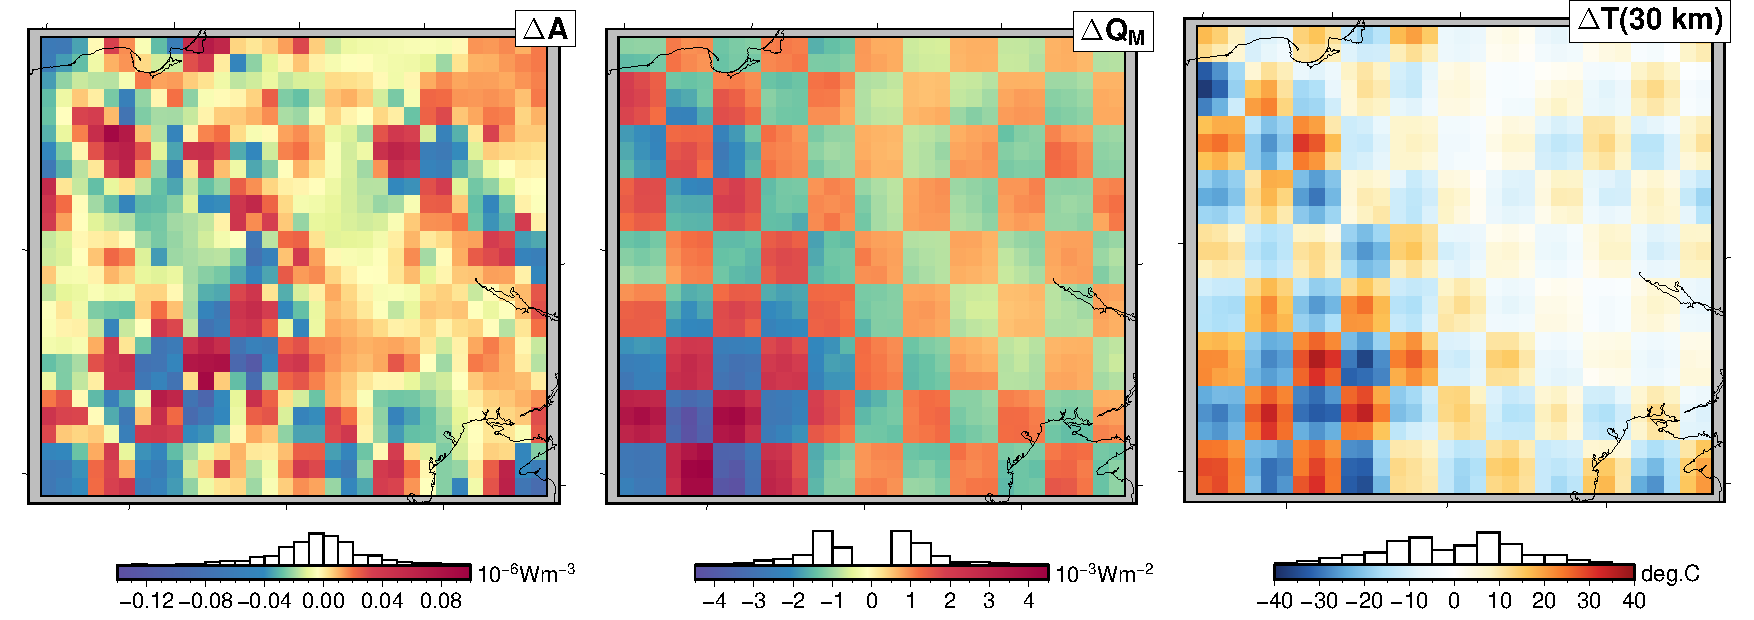
\includegraphics[width=1.35\textwidth]{./0400/CheckMoho_arrays.pdf}}
	\end{adjustbox}
	\caption[Checkerboard Moho test.]{Checkerboard Moho test. Differences in bulk crustal RHP ($\Delta A$), basal heat flow ($\Delta Q_M$), and temperature at \SI{30}{\kilo \metre} depth ($\Delta T(\SI{30}{\kilo \metre})$) are expressed as flat Moho (\SI{44}{\kilo \metre}) minus checkerboard Moho (\num{40} to \SI{48}{\kilo \metre}, \SI{120}{\kilo \metre} square tiles).}
	\label{fig:CompCheckMoho}
\end{figure}

The differences in fitted RHP ($\Delta A$, left map of Fig.~\ref{fig:CompCheckMoho}) are at most one order of magnitude smaller than the range of variation in RHP observed in the model (Fig.~\ref{fig:Aresults}).
In the majority of cases, a difference of $\pm$\SI{0.04}{\micro \watt \per \cubic \metre} in RHP per unit of volume is enough to compensate a $\pm$\SI{4}{\kilo \metre} variation in crustal thickness.
The RHP increases (negative difference) for a thinner crust.
The sensitivity of RHP fitting with respect to the Moho model seems low --this is an expected consequence of all the non crust-correlated RHP variance that I had fitted for.
Larger values (in absolute terms) are observed in cells where the $Q_C:Q_0$ indicates a thermal regime dominated by the crustal contribution (larger values in the right map of Fig.~\ref{fig:QM}).

Differences in basal heat flow ($\Delta Q_M$, central map of Fig.~\ref{fig:CompCheckMoho}) are of comparable magnitude to those observed in the thermal model (Fig.~\ref{fig:QM}).
A thinner crust results in an increased $Q_M$, and vice versa.
There is a subtle variation superimposed on the checkerboard pattern, which becomes more evident in the temperature differences ($\Delta T(30~\mathrm{km}$, right map of Fig.~\ref{fig:CompCheckMoho}).
These are distributed in a zero-average $\pm$\SI{37}{\celsius} range.
A thinner crust tile results in increased temperature, and vice versa, following the same pattern observed with $Q_M$.
The differences attenuate from a full-range alternating pattern in the south-west portion of the area to almost zero in the north-east part.
In contrast to what I observed with $\Delta A$, there is no evident relationship with $Q_C:Q_0$, while the controlling factors appear to be the lithospheric thickness and surface heat flow (which are correlated).

I also tested the effect of using a different crustal model: the seismic Moho by \textcite{Grad2009}, that I had already compared with the satellite-only estimate presented in this chapter, in Fig.~\ref{fig:MohoComparisons} and discussed in section~\ref{ss:Appl:DiscGravMoho}.
In Fig.~\ref{fig:CompGradMoho} I have plotted the differences of three modelling outputs, using the same scheme of the `checkerboard Moho' figure.
Those differences are expressed as: results using my Moho estimate minus results using \textcite{Grad2009}, i.e. a negative difference where the latter results in a larger value.

\begin{figure}
	\begin{adjustbox}{center}
	\fbox{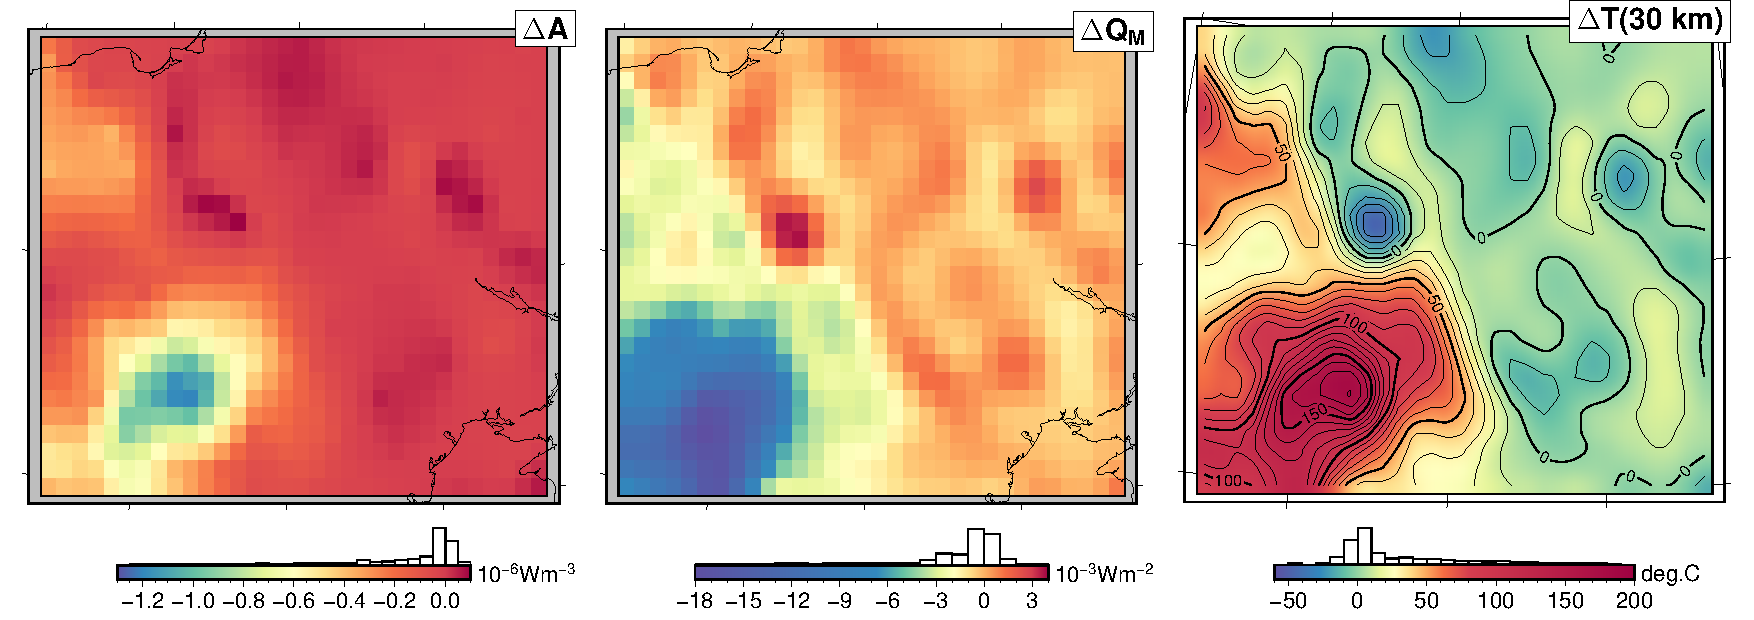
\includegraphics[width=1.35\textwidth]{./0400/GradMoho_arrays.pdf}}
	\end{adjustbox}
	\caption[Thermal results comparison between my Moho model and the one by \textcite{Grad2009}.]{Thermal results comparison between my Moho model and the one by \textcite{Grad2009}. Differences in bulk crustal RHP ($\Delta A$), basal heat flow ($\Delta Q_M$), and temperature at 30~\si{\kilo \metre} depth ($\Delta T(30~\mathrm{km})$) are expressed as results using my Moho minus results using the compared one. The south-west checkerboard tile is a thin tile (40~\si{\kilo \metre}).}
	\label{fig:CompGradMoho}
\end{figure}

In the $\Delta A$ map of Fig.~\ref{fig:CompGradMoho}, I observe a local minimum of \SI{1.2}{\micro \watt \per \cubic \metre} in the Pannonian Basin.
The shallower Moho by \textcite{Grad2009} (24.4~\si{\kilo \metre} minimum, compared to 39.9~\si{\kilo \metre} in my Moho model) has been compensated with an higher RHP, to obtain the same $Q_C$ with a smaller crustal volume.
There are localised spots of positive $\Delta A$, corresponding to structures where the inverted Moho model is thinner (see A) column plots in Fig.~\ref{fig:MohoComparisons}).
The $Q_M$ and $\Delta T(30~\mathrm{km}$ maps show a similar pattern: the thinner crust of \textcite{Grad2009} results in more basal heat flow under the Pannonian Basin and higher temperatures, up to \SI[retain-explicit-plus]{+180}{\celsius}.

Crustal geometry therefore exerts significant effect on heat transport and temperature distribution, and, to a lesser extent, on the results of RHP fitting.
Therefore, a reliable crust estimate appears of utmost importance in their modelling and in their applications, such as thermo-rheological forward modelling \parencite[e.g. ][]{Burov1995}.

\section{Conclusions}
\label{s:Appl:Concl}

I have presented the outcome of a comprehensive gravity-thermal strategy: from the geophysical data reduction of a global gravity model relying on GOCE observations to a regional-scale estimate of crustal thickness, which I then included in a steady-state thermal forward model and a subsequent substitution radioactive heat production fitting technique.
The inverted crustal thickness estimate and the available surface heat flow measurements acted as main constraints.

The gravity reductions that I computed and applied involve global modelling, through a combination of space-domain forward modelling and spectral-domain filtering to ensure full spectral consistency with the band-limited global gravity model.
The Moho undulations that I obtained by inversion of the anomaly that I isolated resulted in a crustal thickness model which resolves most of the features found in the three benchmarks \parencites{Grad2009}{Reguzzoni2015}{Pasyanos2014}, albeit with discrepancies arising from differences in methods and data.

The results show consistency with the thermal regime of the study region, a test box across the Trans-European Suture Zone, at a similar spatial scale as sensed by the gravity model.
Control of the Moho undulations on the temperature distribution is evident, both in terms of heat production and in shaping the mantle-to-surface heat transport, including the effect thermal refraction around hotter and less conductive crustal bodies.

Overall, the suitability of a satellite gravity data to thermal model work flow was assessed.
It is providing useful quantitative insights even when integration with other data is kept to a minimum.
The unparalleled spatial homogeneity in sampling and data quality that satellite-only global gravity models provide is already used to estimate crustal thickness in areas devoid of surface data.
This test has shown how the same approach can be extended to thermal modelling, improving the models of poorly covered areas.

A pitfall of crustal thickness inversion from gravity models is the omission of structures that are instead resolved by seismic methods, due to unmodelled parameters (e.g. density variations) and uncertainties in data reductions.
In the test presented in this chapter I deliberately avoided hard constraints from the seismic Moho models available in the area.
The effects of the discrepancies between this gravity-inverted Moho estimate and the model by \textcite{Grad2009} was assessed in terms of thermal modelling results.
The outcome indicated how the Moho depth is more critical the higher the reduced heat flow ($Q_M$) is, resulting in significant differences under part of the study area.
While the magnitude of this difference is not detrimental to the thermal model reliability, it suggests that an accompanying uncertainty estimate would be beneficial.

Overall, the thermal modelling strategy designed and presented here as a proof of concept has proven fit for its purpose.
The non-uniqueness in heat flow isolation (separating the crustal radiogenic contribution from other concurring thermal factors, such as basal heat flow, long wavelength near surface effects, and tectonic transients) calls for a multivariate inversion problem.
This could be addressed by using an adequate scheme, such as Bayesian inversion \parencite{Mosegaard1995} --which is already commonly adopted in multi-observable lithospheric modelling \parencite[e.g ][]{Mather2018}-- and by including other temperature-dependent constraints, such as the effective elastic thickness \parencite{Burov1995}.

% supplementary material
\cleardoublepage
\begin{subappendices}
\section[Behaviour of the thermal fitting method]{Behaviour of the thermal fitting method}
\label{s:ApplSup:MethodTests}

\subsection{Stability of iterations to account for the temperature dependence of thermal conductivity}
\label{ss:ApplSup:MethodTests:ItStab}
% include "Iterative fitting of radioactive heat production" in this subsection

Temperature dependence of thermal conductivity ($k(T)$) is accounted for using a \textit{subsequent substitution} procedure \parencite[``Picard's method'', see e.g. ][]{Hauck1999}, as described in section~\ref{sss:Appl:ThermCondTdep}.
Every forward call to the thermal model has been run by stopping at the third $k(T)$ substitution iteration.
This means that a first-guess run (`iteration zero') was performed using thermal conductivity ($k$) computed from a linear geotherm (surface temperature to \SI{1200}{\celsius} LAB).
Then, the temperature resulting from the solution of `iteration zero' was used to calculate $k$ of the first iteration, and so on.
Here I have tested the behaviour of $k$ and $T$ through iterations, using a synthetic 1D~column of lithosphere.
Figure~\ref{fig:kITN1} shows the results with a linear first-guess geotherm, while a different first-guess was used in Figure~\ref{fig:kITN2}.
The latter is defined by two segments: first from the surface to a mid-crustal boundary (22~\si{\kilo \metre}) set at \SI{550}{\celsius}, then from there to the \SI{1200}{\celsius} LAB.
The iteration-counting convention adopted here is such as at the $n$-th iteration I am using the $k_n$ calculated using the temperature at iteration $n-1$.
In the figures I show how:
(a) Variations in $k(T)$ and $T$ are strongly attenuated after iteration one. Their values at that point are already smaller than parameter uncertainty.
(b) Two different first-guess linear geotherms converge to the same results, regardless of under- or over-shooting the final geotherm (Fig.~\ref{fig:kITN1} and \ref{fig:kITN2}, respectively). The temperature differences at the 6th iteration is shown in figure~\ref{fig:kITNdiff}: they are on the order of \SI{e-5}{\kelvin}.

\begin{figure}
	\begin{adjustbox}{center}
	\fbox{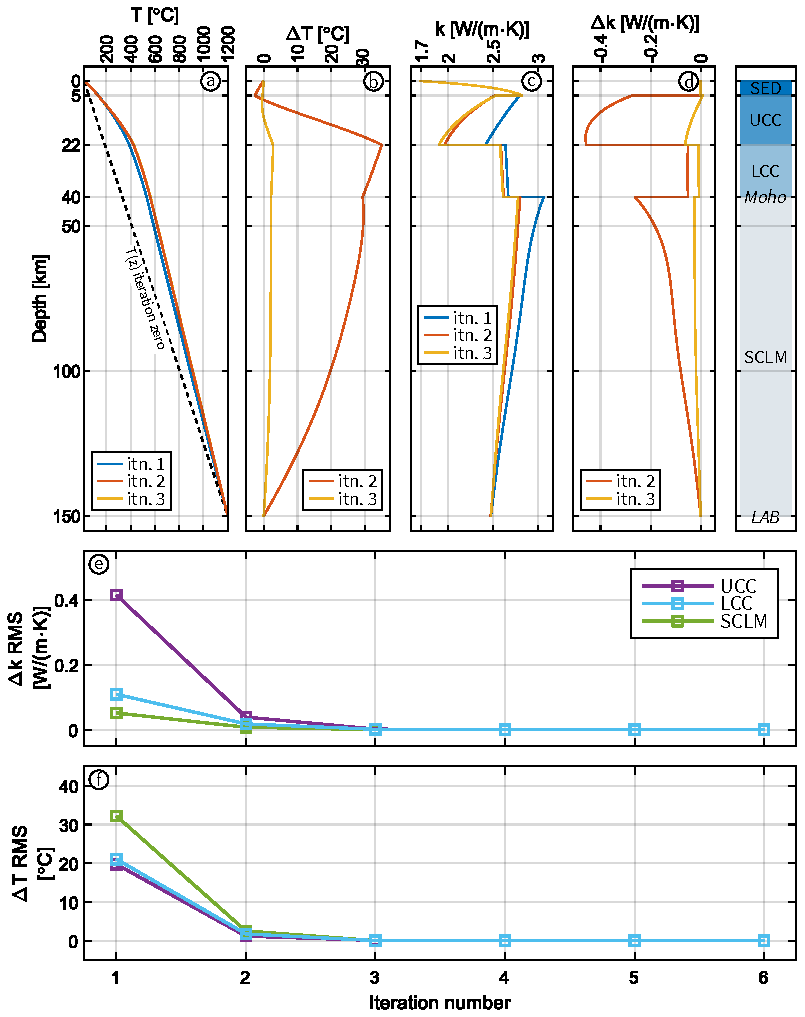
\includegraphics[width=\textwidth]{./0400_suppl/k_itn_case1.pdf}}
	\end{adjustbox}
	\caption[Iterative modelling of temperature-dependent thermal conductivity: linear geotherm.]{Iterative modelling of temperature-dependent thermal conductivity. Case~1: first guess with a linear geotherm. \textbf{a)}~geotherm curve, \textbf{b)}~temperature difference in respect to previous iteration, \textbf{c)}~thermal conductivity, \textbf{d)}~thermal conductivity difference in respect to previous iteration, \textbf{e)}~root mean square of difference in $k$ with previous iteration, separated for the 3 layers with temperature-dependent thermal conductivity, \textbf{f)}~same as e), for temperature. SED: sediments, UCC: upper crystalline crust, LCC: lower crystalline crust, SCLM: sub-continental lithospheric mantle.
	Plots a) through d) stop at the third iteration, the subsequent variations are too small to be visualised. The difference between $T$ of iteration 1 and the first guess is not shown.}
	\label{fig:kITN1}
\end{figure}

\begin{figure}
	\begin{adjustbox}{center}
	\fbox{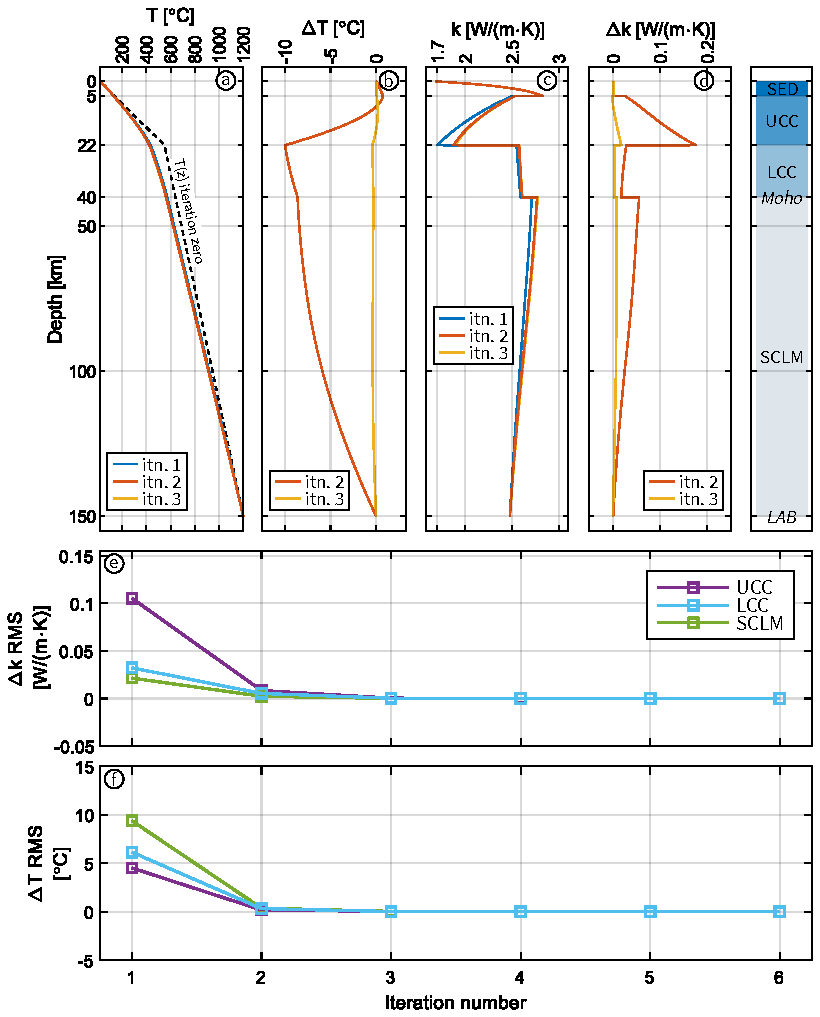
\includegraphics[width=\textwidth]{./0400_suppl/k_itn_case2.pdf}}
	\end{adjustbox}
	\caption[Iterative modelling of temperature-dependent thermal conductivity: segmented geotherm.]{Iterative modelling of temperature-dependent thermal conductivity. Case~2: first guess with a segmented geotherm.
	Description: see caption of Fig.~\ref{fig:kITN1}.}
	\label{fig:kITN2}
\end{figure}

\begin{figure}
	\begin{adjustbox}{center}
	\fbox{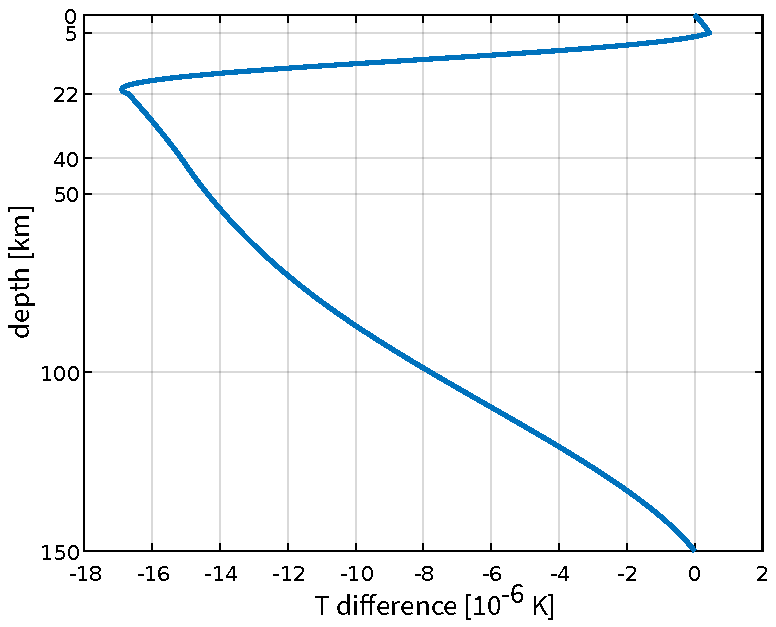
\includegraphics[width=0.75\textwidth]{./0400_suppl/k_itn_Tguess_diff.pdf}}
	\end{adjustbox}
	\caption[Iterative modelling of temperature-dependent thermal conductivity: differences.]{Iterative modelling of temperature-dependent thermal conductivity: difference between geotherms obtained with the first guess of case~1 (Fig.~\ref{fig:kITN1}) and case~2 (Fig.~\ref{fig:kITN2}).
	Note the less than significant order of magnitude.}
	\label{fig:kITNdiff}
\end{figure}

\FloatBarrier

\subsection{Iterative fitting of radioactive heat production}
\label{ss:ApplSup:MethodTests:ItFit}
In figures~\ref{fig:AITN_ACC} trough~\ref{fig:AITN_DAC} I am showing the output of the fitting procedure (section~\ref{ss:Appl:ThermRHP}), iteration by iteration.
``Iteration zero'' refers to the first-guess radioactive heat production (RHP) value, which is used to run the first forward model.
It is constant throughout the area (\textbf{A\textsubscript{C}~0} map, Fig.~\ref{fig:AITN_ACC}).

In these maps the crustal heat production is expressed as one \textit{bulk value}.
Throughout the adopted strategy, this value is partitioned between the upper and lower crystalline crust using a reference ratio.
The increasing trend in the range of RHP values is described and discussed in section~\ref{ss:Appl:DiscTherm:FWD}, where it is summarised with a plot (Fig.~\ref{fig:RMSvsITN}) of the RMS value for each iteration and maps at iteration zero and six only.
Here it si plotted for all the iterations.

The ``$Q_M$ suppression'' is shown in Fig.~\ref{fig:AITN_Qm}.
By comparing those maps with those of the crustal component of heat flow ($Q_C$, Fig.~\ref{fig:AITN_Qc}, computed as heat flow at the sediment-crystalline crust interface minus heat flow at the crust-mantle interface), I can identify a progressive reduction in $Q_M$ in areas of increasing crustal heat production.

As described before (section~\ref{ss:Appl:ThermRHP}), I have chosen this iterative fitting strategy due to the concurring behaviour of the temperature dependence of thermal conductivity and the non-horizontal heat conduction phenomena arising in a truly 3D thermal model.
I recall that in a 1D model (i.e. only vertical conduction, column-wise), I could compute the RHP per unit of volume in the crust dividing the crustal component of surface heat flow (stripped from other contributions) by the crustal thickness.
In Fig.~\ref{fig:AITN_A1D} I show the value of crustal RHP that results from doing so.
I computed it a-posteriori, after each thermal forward model run.
In Fig.~\ref{fig:AITN_DAC} I show the difference between the actual values used in the model, iteration by iteration, and the ones obtained using the aforementioned `1D~approximation'.
Differences correlate with the actual (i.e. modelled) RHP values, but sharp variations are observed where lateral variations in RHP or in Moho depth occur, resulting in departure from vertical conduction.

\FloatBarrier

\begin{figure}
	\begin{adjustbox}{center}
	\fbox{
		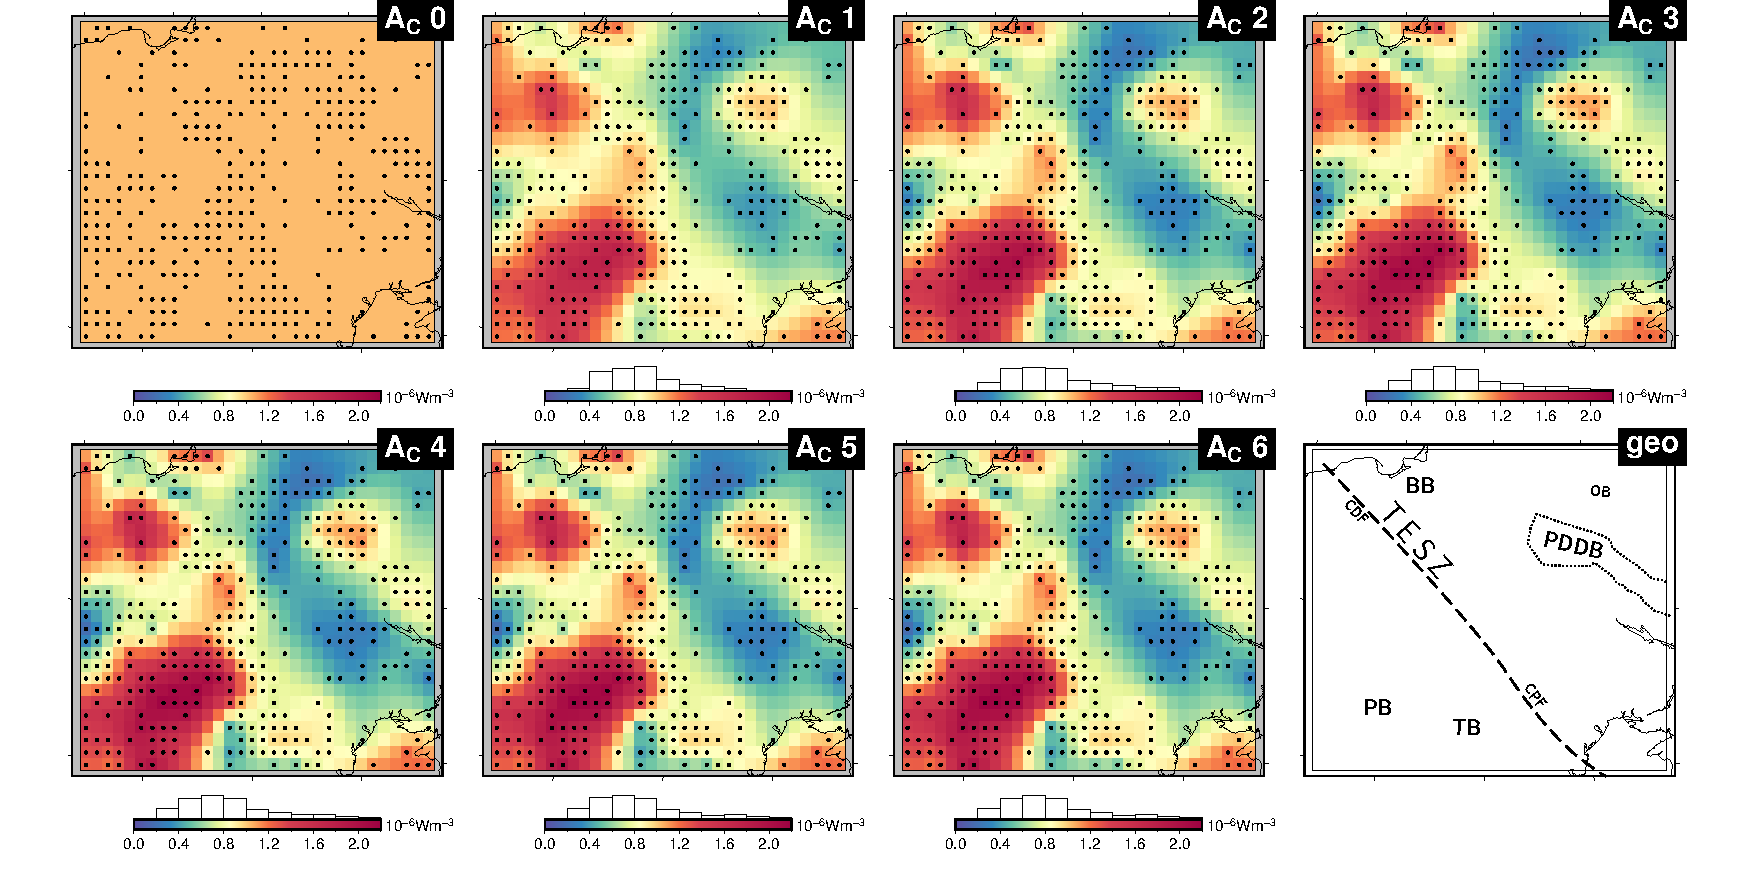
\includegraphics[
			clip, trim=1cm 0.6cm 1cm 0.05cm,
			width=1.3\textwidth]{./0400_suppl/ACCarrays.pdf}
		}
	\end{adjustbox}
	\caption[Bulk heat production of the crystalline crust, all iterations.]{Value of bulk heat production of the crystalline crust, trough the fitting iterations.}
	\label{fig:AITN_ACC}
\end{figure}

\begin{figure}
	\begin{adjustbox}{center}
	\fbox{
		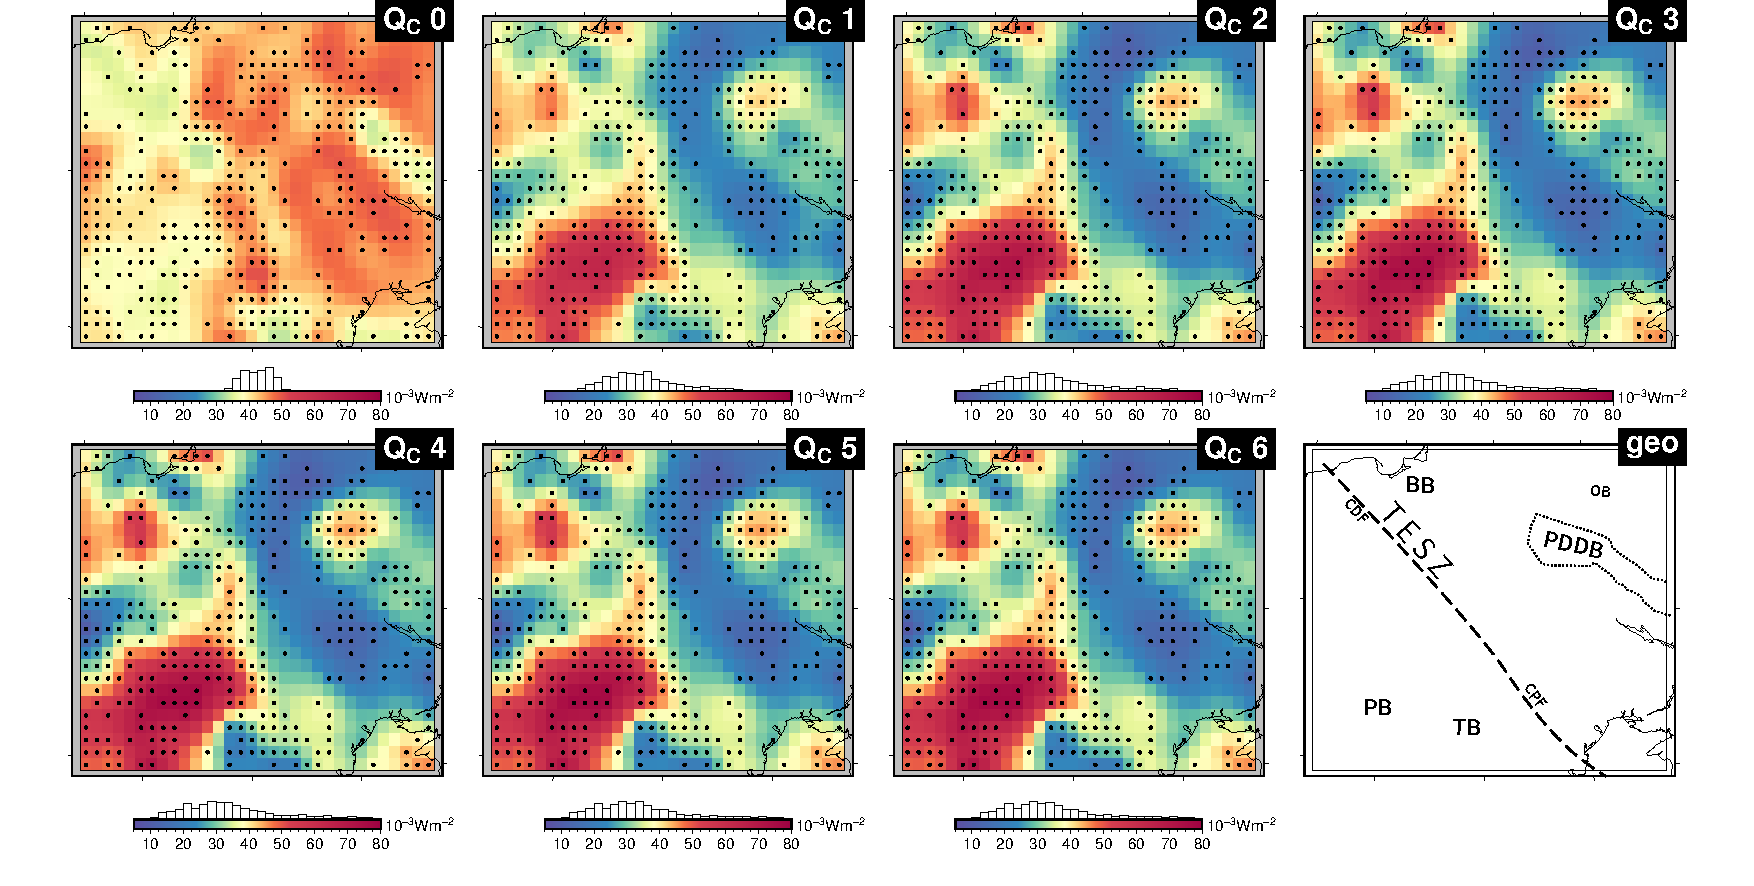
\includegraphics[
			clip, trim=1cm 0.6cm 1cm 0.05cm,
			width=1.3\textwidth]{./0400_suppl/Qc_arrays.pdf}
		}
	\end{adjustbox}
	\caption[Crustal contribution to the surface heat flow, all iterations.]{Crustal contribution to the surface heat flow, computed as heat flow at the sediment-crystalline crust interface minus heat flow at the crust-mantle interface, trough the fitting iterations.}
	\label{fig:AITN_Qc}
\end{figure}

\begin{figure}
	\begin{adjustbox}{center}
	\fbox{
		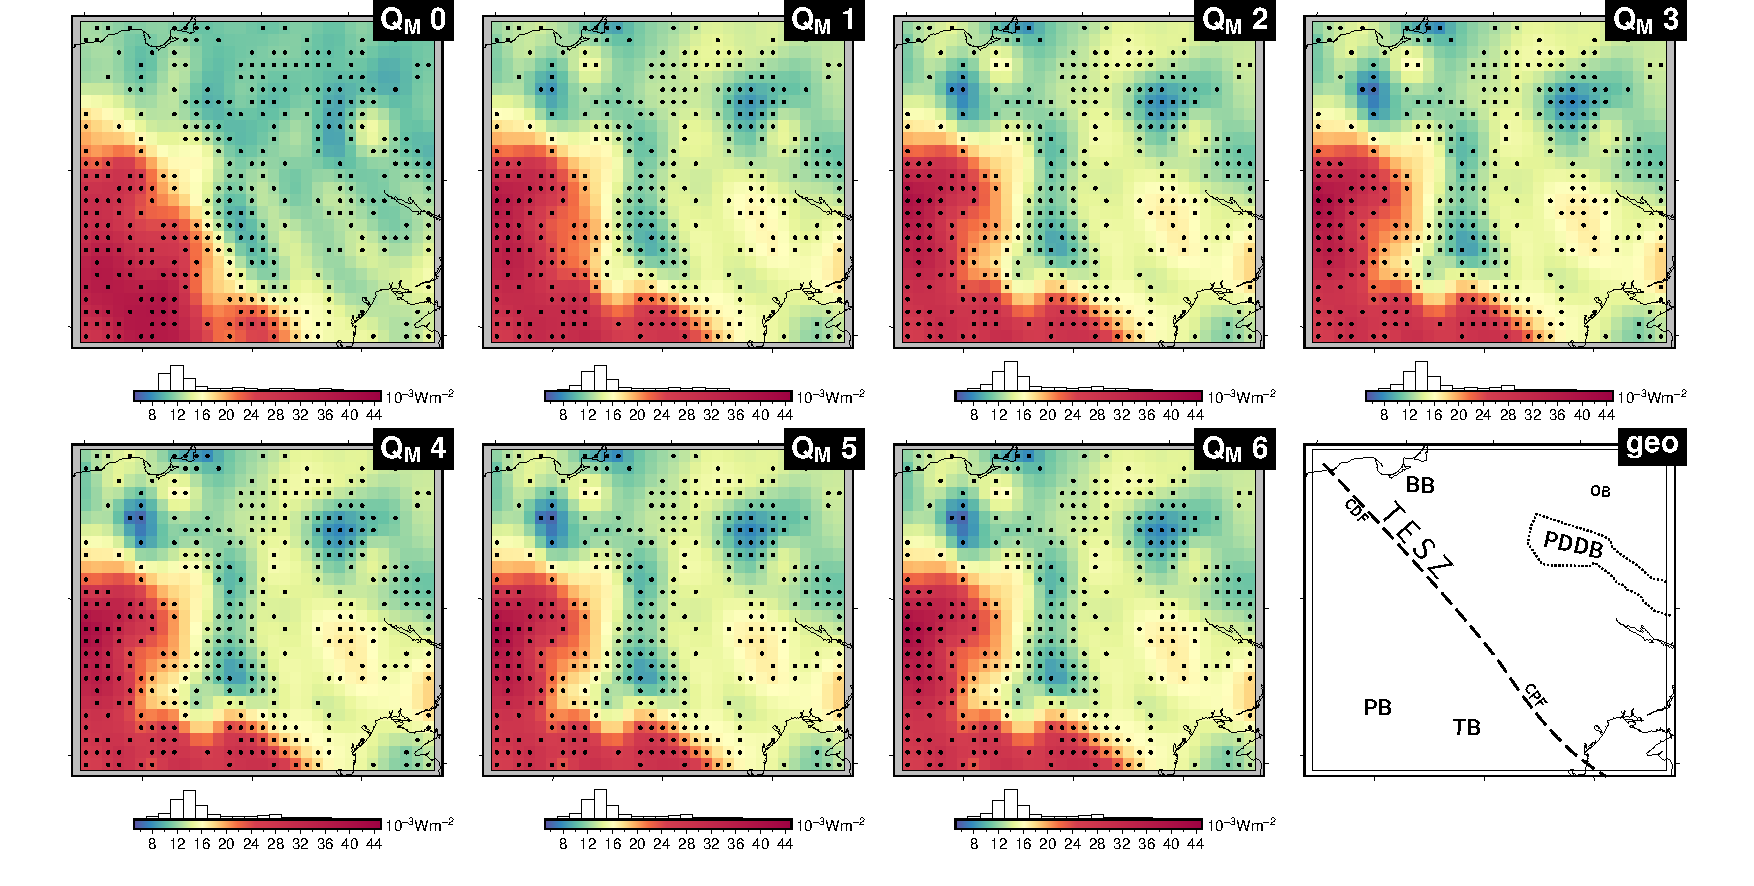
\includegraphics[
			clip, trim=1cm 0.6cm 1cm 0.05cm,
			width=1.3\textwidth]{./0400_suppl/Qm_arrays.pdf}
		}
	\end{adjustbox}
	\caption[Basal heat flow, all iterations.]{Heat flow at the crust-mantle interface (basal heat flow), trough the fitting iterations.}
	\label{fig:AITN_Qm}
\end{figure}

\begin{figure}
	\begin{adjustbox}{center}
	\fbox{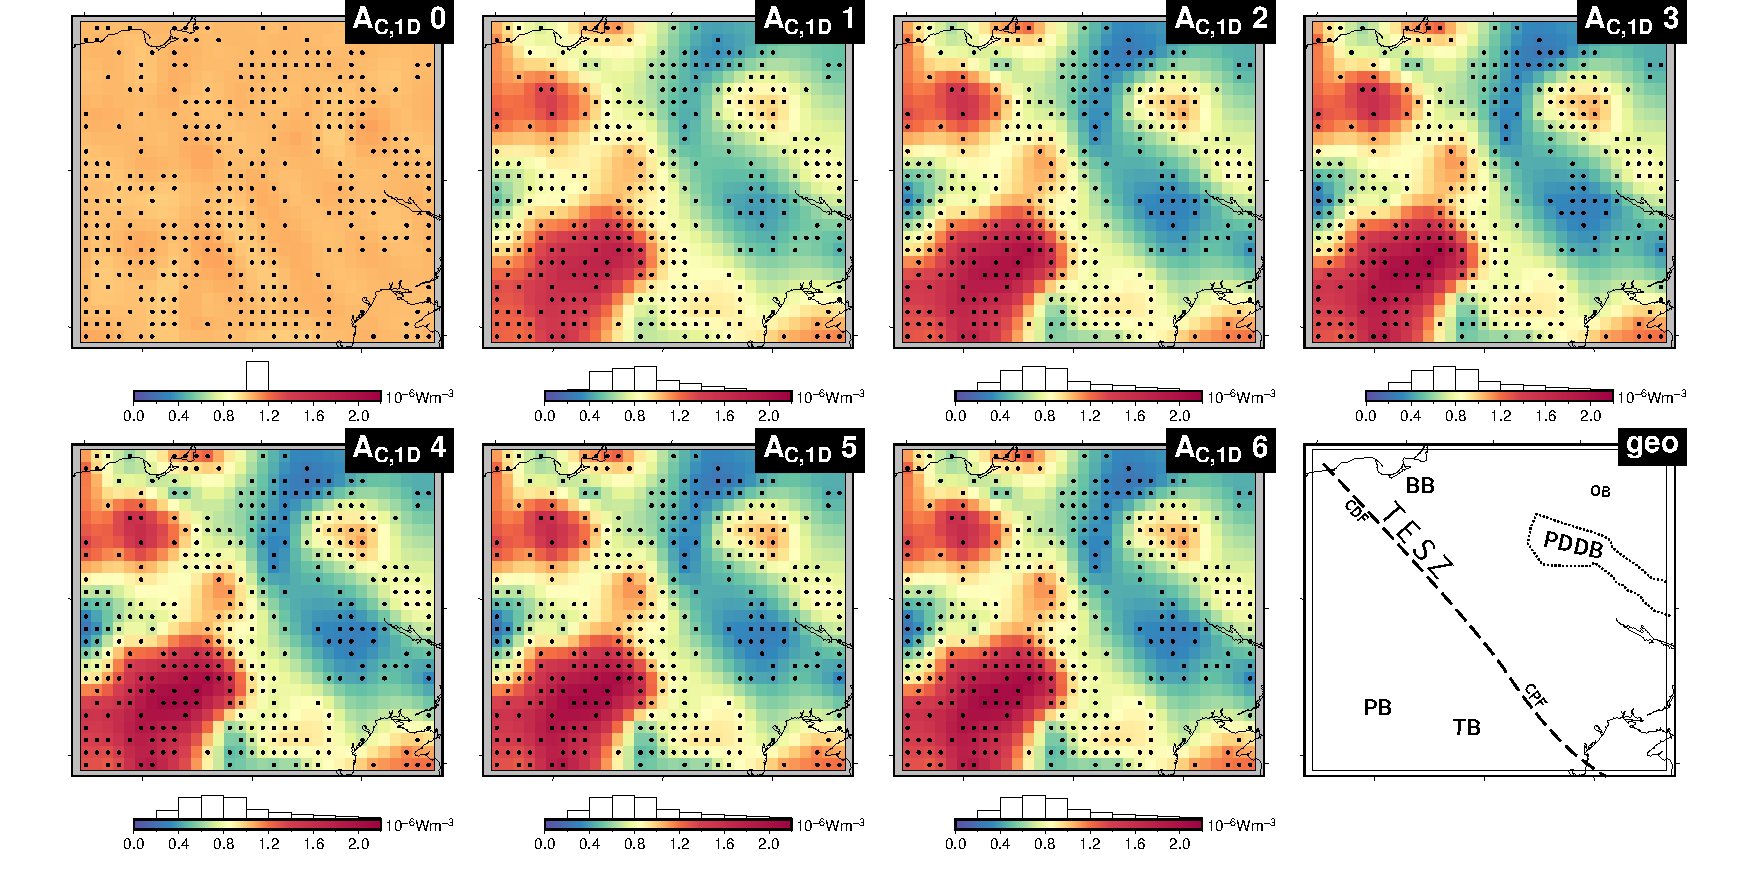
\includegraphics[
		clip, trim=1cm 0.6cm 1cm 0.05cm,
		width=1.3\textwidth]{./0400_suppl/A1Darrays.pdf}
		}
	\end{adjustbox}
	\caption[Crustal heat production computed a-posteriori, using a 1D approximation.]{Crustal heat production computed a-posteriori using a 1D approximation, i.e. crustal heat flow divided by crustal thickness.}
	\label{fig:AITN_A1D}
\end{figure}

\begin{figure}
	\begin{adjustbox}{center}
	\fbox{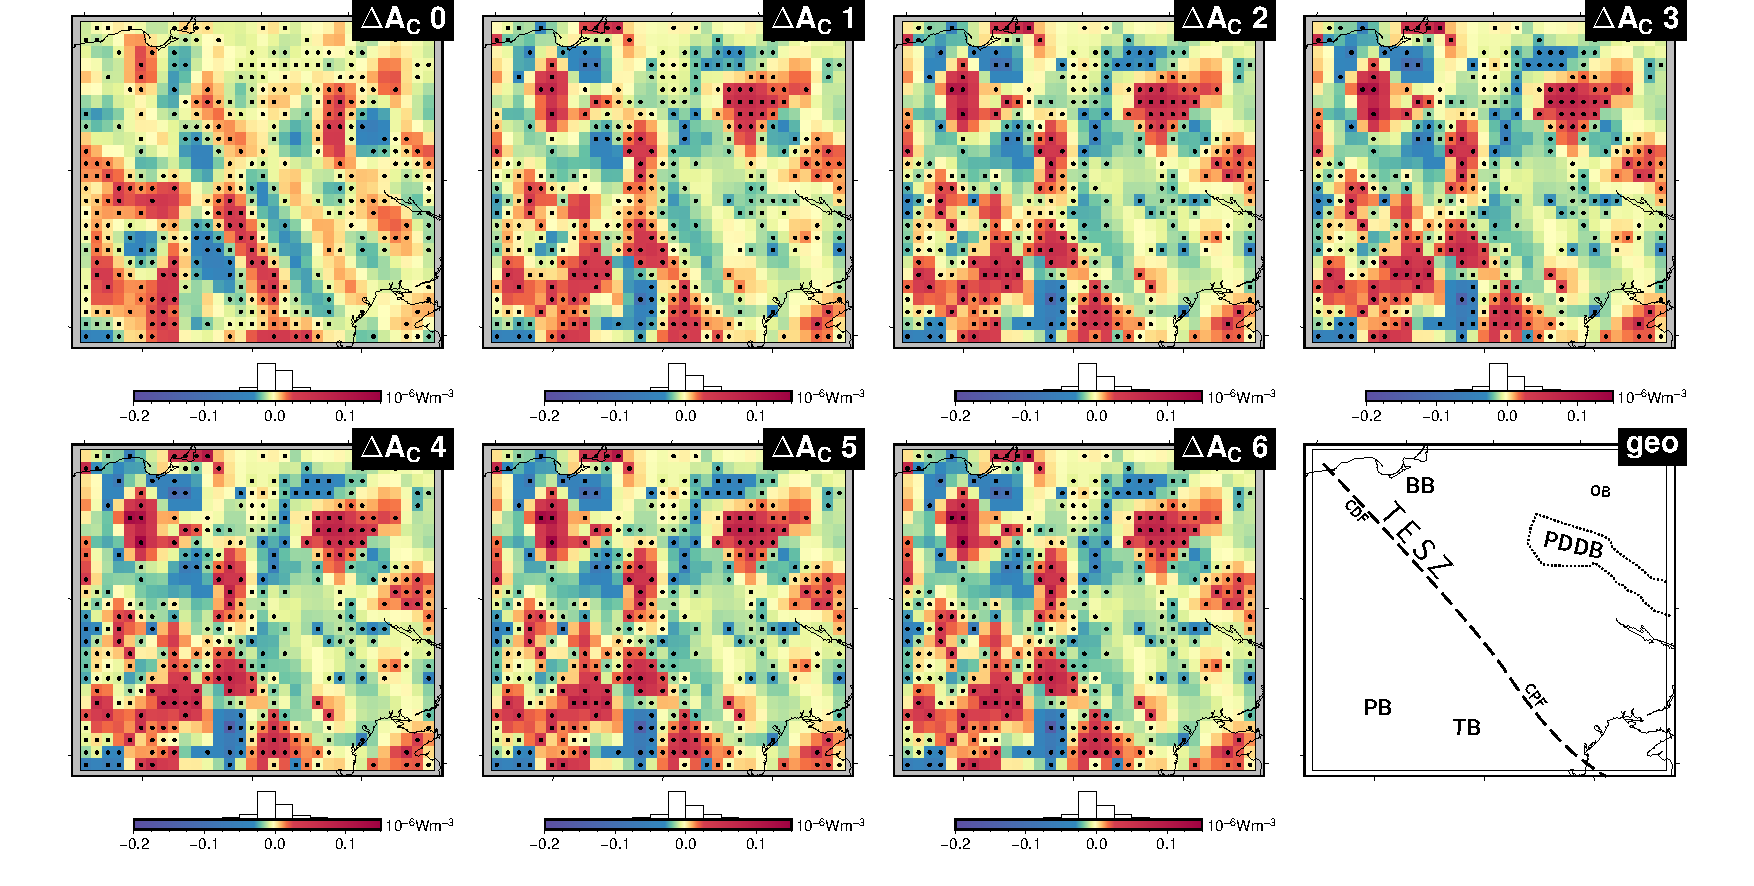
\includegraphics[
		clip, trim=1cm 0.6cm 1cm 0.05cm,,
		width=1.3\textwidth]{./0400_suppl/DACarrays.pdf}}
	\end{adjustbox}
	\caption[Difference between the model RHP and the 1D-approximation.]{Difference between the crustal heat production as used in the 3D model (Fig.~\ref{fig:AITN_ACC}), and the a-posteriori 1D-computed heat production (Fig.~\ref{fig:AITN_A1D}).}
	\label{fig:AITN_DAC}
\end{figure}

\FloatBarrier

\subsection{Effects of horizontal heat conduction}
\label{ss:ApplSup:MethodTests:HorQ}

I include the result of a synthetic experiment showing the significance of non-vertical heat conduction.
The forward model is parametrised with the same reference conductivity and heat production (first-guess) values previously presented in section~\ref{s:Appl:Therm} and Tab.~\ref{tab:ThermParams}.
It consists of a 600~\si{\kilo \metre} 2D x-z section.
It is one-element thick along the y axis (normal to the section) and a zero-flux conditions is imposed on the front and back sides (y-wise).
Therefore, it represent a model of infinite extent along the y-axis.
The grid step is 1~\si{\kilo \metre} and 50~m along x and z, respectively.
No grid step coarsening has been applied along z, owing to the small model size in terms of computational budget.
The results are shown in Fig.~\ref{fig:2Deff}.

The model geometry includes a step in the crustal thickness: the undisturbed Moho is 40~\si{\kilo \metre} deep, while the it reaches 48~\si{\kilo \metre} in the thickened part, in the section center.
The upper-lower crust boundary is set proportionally.
In the left side of the section the step is a sharp transition, taking place from one model node to the next.
In the right side it was smoothed with a Gaussian filter (100~\si{\kilo \metre} cutoff wavelength).
The sediment basement and the LAB are flat, at 4~\si{\kilo \metre} and 100~\si{\kilo \metre} respectively.
The topography is also flat.
Three $k(T)$ iterations were used.

Plot \textbf{a)} of Fig.~\ref{fig:2Deff} represents the surface heat flow, computed from the temperature section using the following:

\begin{equation}
    Q_0 = \frac{T(z_1) - T(z_0)}{z_1 - z_0} \cdot \frac{k(z_1) + k(z_0)}{2}
\label{eq:HF}
\end{equation}
Where $z_0$ and $z_1$ are the $z$-coordinate of the surface and first sub-surface node, respectively. $z$ is defined positive downwards.
The second term of the product is an arithmetic mean of the thermal conductivities of the two nodes.
This numerical vertical heat flow resembles a near-surface heat flow measurement in a well, under ideal conditions.
In plot \textbf{b)} of Fig.~\ref{fig:2Deff}, I am comparing $Q_C$ obtained by two methods:
\begin{description}
	\item[2D, blue curve:] the crustal component of surface heat flow derived from the model, computed as a difference between the heat flow at the sediment basement (boundary between `SEDS' and `UCC' layers) and the basal heat flow (boundary between `LCC' and `SCLM' layers). This follows the same convention outlined in eq.~\ref{eq:HF};
	\item[1D, orange curve:] the crustal component computed as the integral of crustal heat production per unit of volume along the crustal thickness. This  resembles a 1D, column-wise, model. Notice the different response to the sharp step (left side).
\end{description}
In plot \textbf{c)} of Fig.~\ref{fig:2Deff}, I am comparing $Q_M$ obtained by two methods:
\begin{description}
	\item[2D, blue curve:] the basal heat flow as numerical heat flow at the Moho (boundary between `LCC' and `SCLM' layers);
	\item[1D, orange curve:] basal heat flow interpreted as `reduced heat flow' in a 1D approach: I subtracted the column-wise 1D $Q_C$ to $Q_0$.
	Notice how the misfit becomes larger near the edges of the thickened crust (both step and smooth transitions), while it is almost zero at its center.
\end{description}

Plot \textbf{d)} of Fig.~\ref{fig:2Deff} shows the temperature field as contours, in degrees Celsius.
The layer structure is plotted in the background.
In plot \textbf{e)} of Fig.~\ref{fig:2Deff} I am showing the deviation from a purely vertical temperature gradient (angle $\alpha$).
It was calculated with the following:

\begin{equation}
    \alpha_i = \mathrm{arctan} \frac{\mathrm{abs}\left(\nabla_x T_i \right)}{\nabla_z T_i}
\label{eq:alpha}
\end{equation}
where $\nabla$ indicates the numerical gradient calculated between nodes of the temperature field.
A sketch is included in the bottom of Fig.~\ref{fig:2Deff}.
To improve the plot clarity, the sign of the horizontal gradient was discarded: its direction is towards negative-$x$ in the left side of the plot, towards positive-$x$ in the right side -- i.e. heat flow is deviated around the thickened, hotter portion of crust.

\begin{figure}
	\begin{adjustbox}{center}
	\fbox{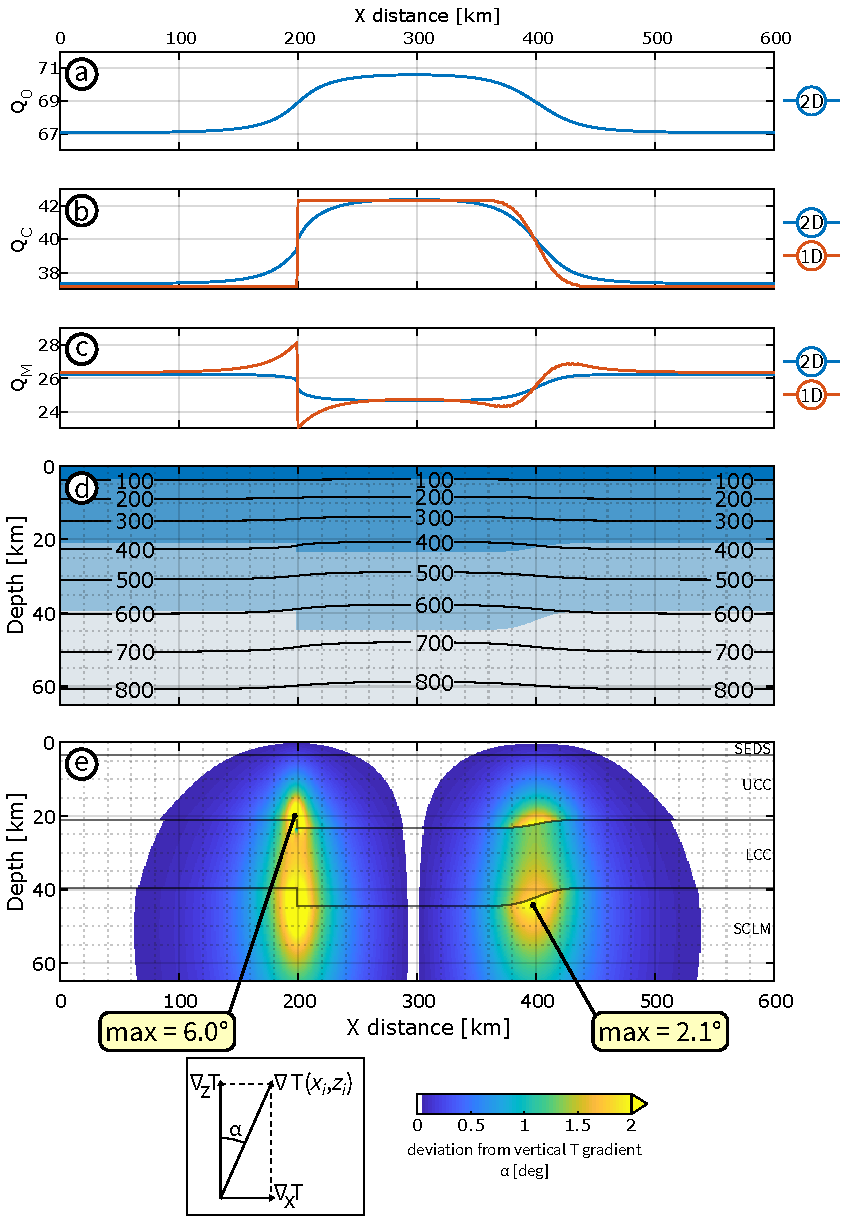
\includegraphics[width=\textwidth]{./0400_suppl/SM2D_effect.pdf}}
	\end{adjustbox}
	\caption[Synthetic experiment showing the effect of horizontal heat conduction.]{Synthetic experiment showing the effect of horizontal heat conduction.}
	\label{fig:2Deff}
\end{figure}

\FloatBarrier

\subsection{Effect of a temperature-dependent Moho density contrast}
\label{ss:ApplSup:MethodTests:MohoDeltaRho}

To assess the effect of temperature on the densities used in the inverted Moho depth estimates, I have tested the effect of re-computing the Moho density contrast using the thermal modelling results.
The densities were updated according to the following, from \textcite{allen2013basin}:

\begin{equation*}
    \rho(T,P) = \rho_0 (1 - \alpha_V \Delta T + \beta P) 
\end{equation*}

where $\rho_0$ is the initial density, $\alpha_V$ the volumetric coefficient of thermal expansion (in \si{\per \kelvin}), $\Delta T$ the change in temperature, $\beta$ compressibility (in \si{\per \pascal}), and $P$ pressure (in \si{\pascal}). I used a $\beta$ of \num{3e-11} and \SI{1e-11}{\per \kelvin} for the crust and lithospheric mantle (assumed peridotite), respectively, and a $\alpha_V$ of \SI{2.4e-5}{\per \pascal} for both the crust and the lithospheric mantle.

The new inverted Moho, in Fig.~\ref{fig:RhoTP_MohoDepth}, shows a variation (after minus before) ranging from \SI{-2.3}{\kilo \metre} to \SI[retain-explicit-plus]{+3.4}{\kilo \metre}, with an average of \SI{-0.13}{\kilo \metre} and a standard deviation of \SI{0.75}{\kilo \metre}.
The range and variance of these discrepancies are less than the typical uncertainties of crustal thickness estimation ($\pm$\num{5} to $\pm$\num{15} percent, i.e. $\pm$\num{2} to $\pm$\SI{6}{\kilo \metre} for a \SI{40}{\kilo \metre} thick crust, see \cite{Grad2009} and references therein).

\begin{figure}
	\begin{adjustbox}{center}
	\fbox{
		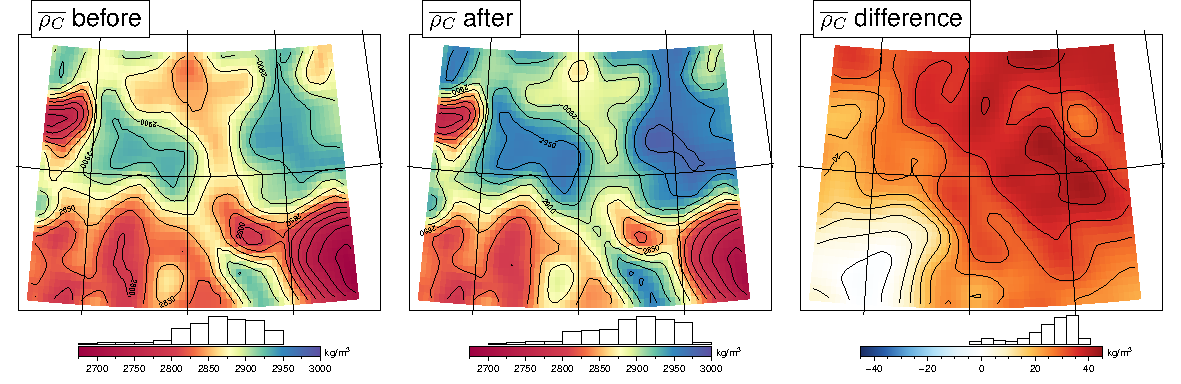
\includegraphics[
			width=1.35\textwidth,
			clip, trim=0.3cm 0.2cm 0.3cm 0cm]{./0400_suppl/RhoTP_RhoC.pdf}
		}
	\end{adjustbox}
	\caption[Bulk density of the crystalline crust, effect of temperature dependence.]{Bulk density of the crystalline crust.
	Left: from LITHO1.0.
	Center: updated with $(T,P)$~effect, with the output of the thermal modelling. 
	Right: $(T,P)$~effect contribution, updated density minus original density.}
	\label{fig:RhoTP_RhoC}
\end{figure}

\begin{figure}
	\begin{adjustbox}{center}
	\fbox{
		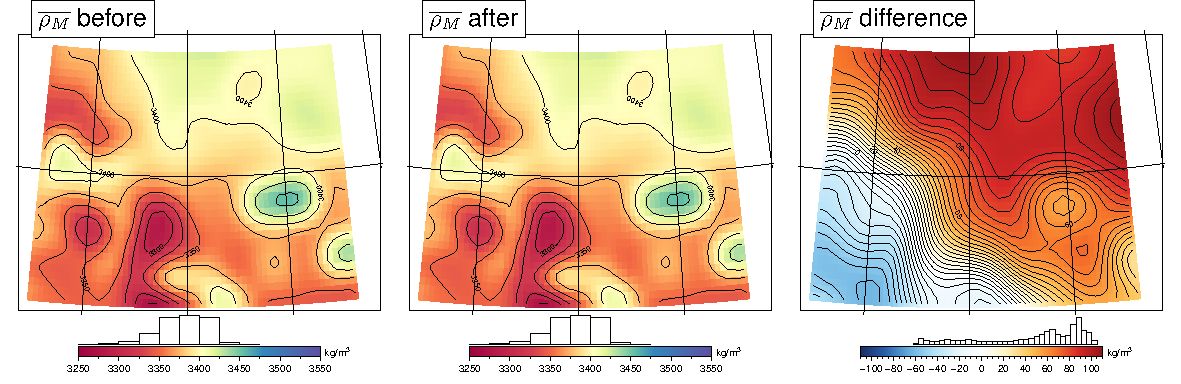
\includegraphics[
			width=1.35\textwidth,
			clip, trim=0.3cm 0.2cm 0.3cm 0cm]{./0400_suppl/RhoTP_RhoM.pdf}
		}
	\end{adjustbox}
	\caption[Bulk density of the lithospheric mantle, effect of temperature dependence.]{Bulk density of the lithospheric mantle.
	Left: from LITHO1.0.
	Center: updated with $(T,P)$~effect, with the output of the thermal modelling.
	Right: $(T,P)$~effect contribution, updated density minus original density.}
	\label{fig:RhoTP_RhoM}
\end{figure}

\begin{figure}
	\begin{adjustbox}{center}
	\fbox{
		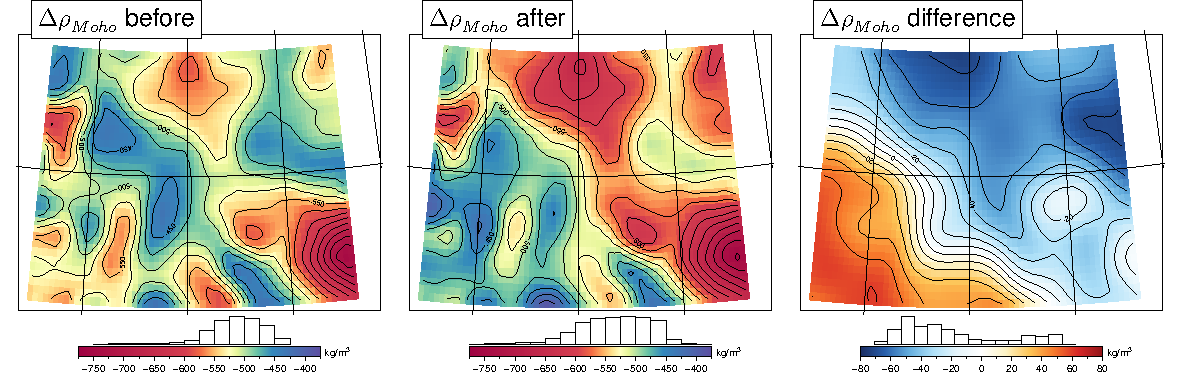
\includegraphics[
			width=1.35\textwidth,
			clip, trim=0.3cm 0.2cm 0.3cm 0cm]{./0400_suppl/RhoTP_MohoContrast.pdf}
		}
	\end{adjustbox}
	\caption[Moho contrast, effect of temperature dependence.]{Moho contrast, expressed as bulk crust density (Fig.~\ref{fig:RhoTP_RhoC}) minus lithospheric mantle bulk density (Fig.~\ref{fig:RhoTP_RhoM}).
	Left: from LITHO1.0.
	Center: updated with $(T,P)$~effect, with the output of the thermal modelling. Right: $(T,P)$~effect contribution, updated density minus original density.}
	\label{fig:RhoTP_MohoContrast}
\end{figure}

\begin{figure}
	\begin{adjustbox}{center}
	\fbox{
		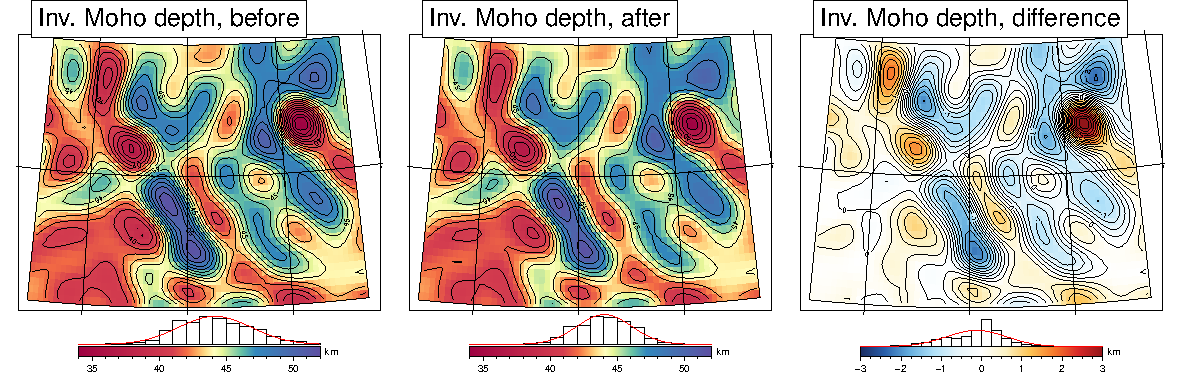
\includegraphics[
			width=1.35\textwidth,
			clip, trim=0.3cm 0.2cm 0.3cm 0cm]{./0400_suppl/RhoTP_MohoDepth.pdf}
		}
	\end{adjustbox}
	\caption[Inverted Moho depth, effect of temperature dependence.]{Inverted Moho depth.
	Left: using the density contrast from LITHO1.0, unmodified.
	Center: using the density contrast updated with $(T,P)$~effect, with the output of the thermal modelling.
	Right: $(T,P)$~effect contribution, updated Moho minus initial Moho estimate.}
	\label{fig:RhoTP_MohoDepth}
\end{figure}

\FloatBarrier

\section[
	tocentry={A-posteriori test of heat production relationships},
	head={A-posteriori test of RHP relationships with other physical properties}]{A-posteriori test of RHP relationships with other physical properties}
\label{s:ApplSup:Rel}

\subsection{Relationship of RHP with density}
\label{ss:ApplSup:Rel:Rho}

Fig.~\ref{fig:RhoRHP} provides an alternate representation of Fig.~\ref{fig:Qcrossplots}.
Instead of the RHP~versus~density scatter plot (upper right axes), here I am including a map of the spatial distribution of the bulk crustal density.
The density of the samples in all the scatter plots (each sample a model column) is plotted with the same colour scale used in the density map.

\begin{figure}
	\begin{adjustbox}{center}
	\fbox{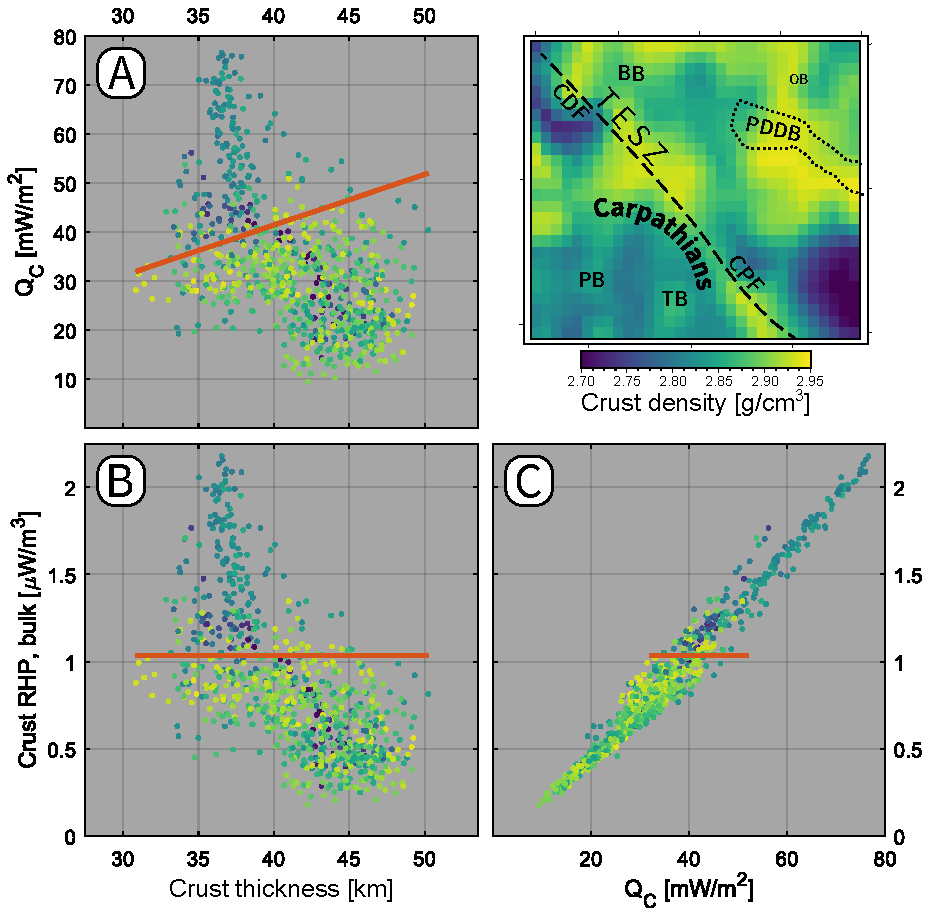
\includegraphics[width=1.2\textwidth]{./0400_suppl/crossplots_rho_mod.pdf}}
	\end{adjustbox}
	\caption[Cross plots: crust thickness, RHP, crustal heat flow, crust density.]{Cross plots between thickness of the crystalline crust (Moho depth minus basement depth), radioactive heat production (RHP) of the bulk crystalline crust, crustal component of heat flow ($Q_C$), and crust density. The line overlaid on scatter~plots \textbf{A)} to \textbf{C)} represents the first guess, using the a-priori constant RHP.
	The map in the upper right shows the bulk crustal density (depth-weighted average) for each model column.}
	\label{fig:RhoRHP}
\end{figure}

\subsection[Relationship of RHP with VP]{Relationship of RHP with V\textsubscript{P}}
\label{ss:ApplSup:Rel:VP}

Fig.~\ref{fig:VpRHP} shows the comparison between the inverted RHP estimate and the output of \parencite{Hasterok2017_ign} V\textsubscript{P}-RHP relationship (using data for the continental crust), as discussed at the end of section~\ref{ss:Appl:DiscTherm:FWD}.
Log-linear fits are in the following form (Eq.~4 in \cite{Hasterok2017_ign}):

\begin{equation*}
	\log_{10} A = m (V_{P} - 6) + b
\end{equation*}
With $m$ in $(\log_{10} (\mu W \ m^{-3})) \ (km \ s^{-1})^{-1}$, $b$ in $\log_{10} (\mu W \ m^{-3})$, $V_{P}$ in $km \ s^{-1}$. \\
Hasterok and Webb (2017) fit parameters (`continental') are: $m = -0.70 \pm 0.10$, $b = 0.48 \pm 0.08$.
The fit I have obtained on data of this chapter (by regression) is: $m = -0.56 \pm 0.18$, $b = 0.19 \pm 0.11$.
Confidence interval provided for $\pm 2 \sigma$.

\begin{figure}
	\begin{adjustbox}{center}
	\fbox{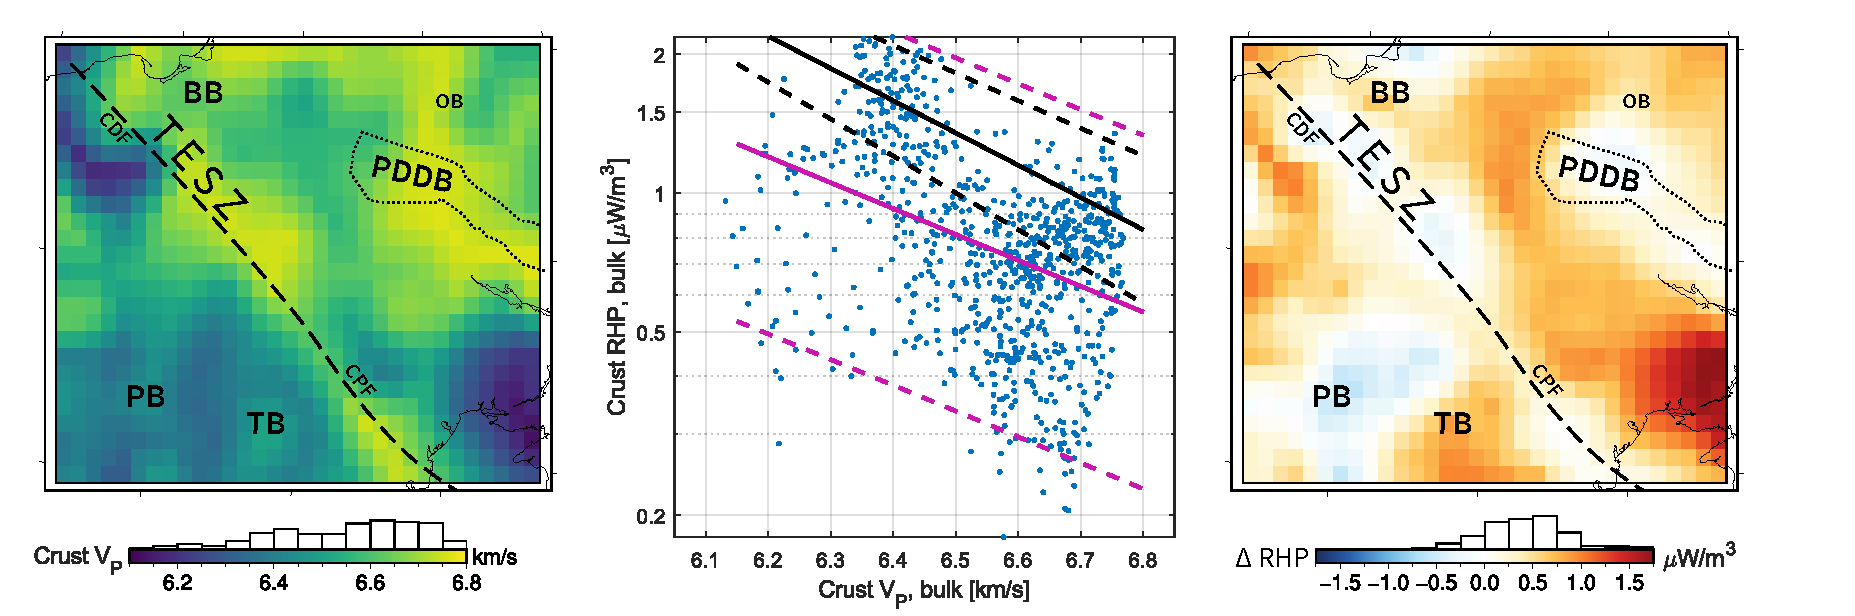
\includegraphics[width=1.35\textwidth]{./0400_suppl/VpRHP.pdf}}
	\end{adjustbox}
	\caption[Relationship of RHP with V\textsubscript{P}, difference with fitted RHP.]{
		\textbf{Left:}~V\textsubscript{P} of the crystalline crust (thickness-weighted average of \cite{Pasyanos2014} data), computed along the nodes of each model column.
		\textbf{Center:}~scatter plot of crustal V\textsubscript{P} against the inverted crustal RHP estimate. The V\textsubscript{P}-RHP relationship by \cite{Hasterok2017_ign} is plotted in black. A log-linear fit to the inverted data is plotted in purple. Dashed lines depict upper and lower confidence bounds ($\pm$2 standard deviations).
		\textbf{Right:}~V\textsubscript{P}-RHP estimate minus the inverted estimate.}
	\label{fig:VpRHP}
\end{figure}

\end{subappendices}
